\chapter{Related Work}
My vision of addressing ICS student problems through an online platform involves three major parts: degree planner, social network, and gamification. All three of these parts combine to create a robust, interactive, and effective system to enhance the academic journeys of current and future ICS students. In this section I discuss existing software in each of these categories, what they aim to accomplish, and why they do not fully satisfy the needs of ICS students.

\section{Degree Planners}
\begin{figure}[h]
\centering
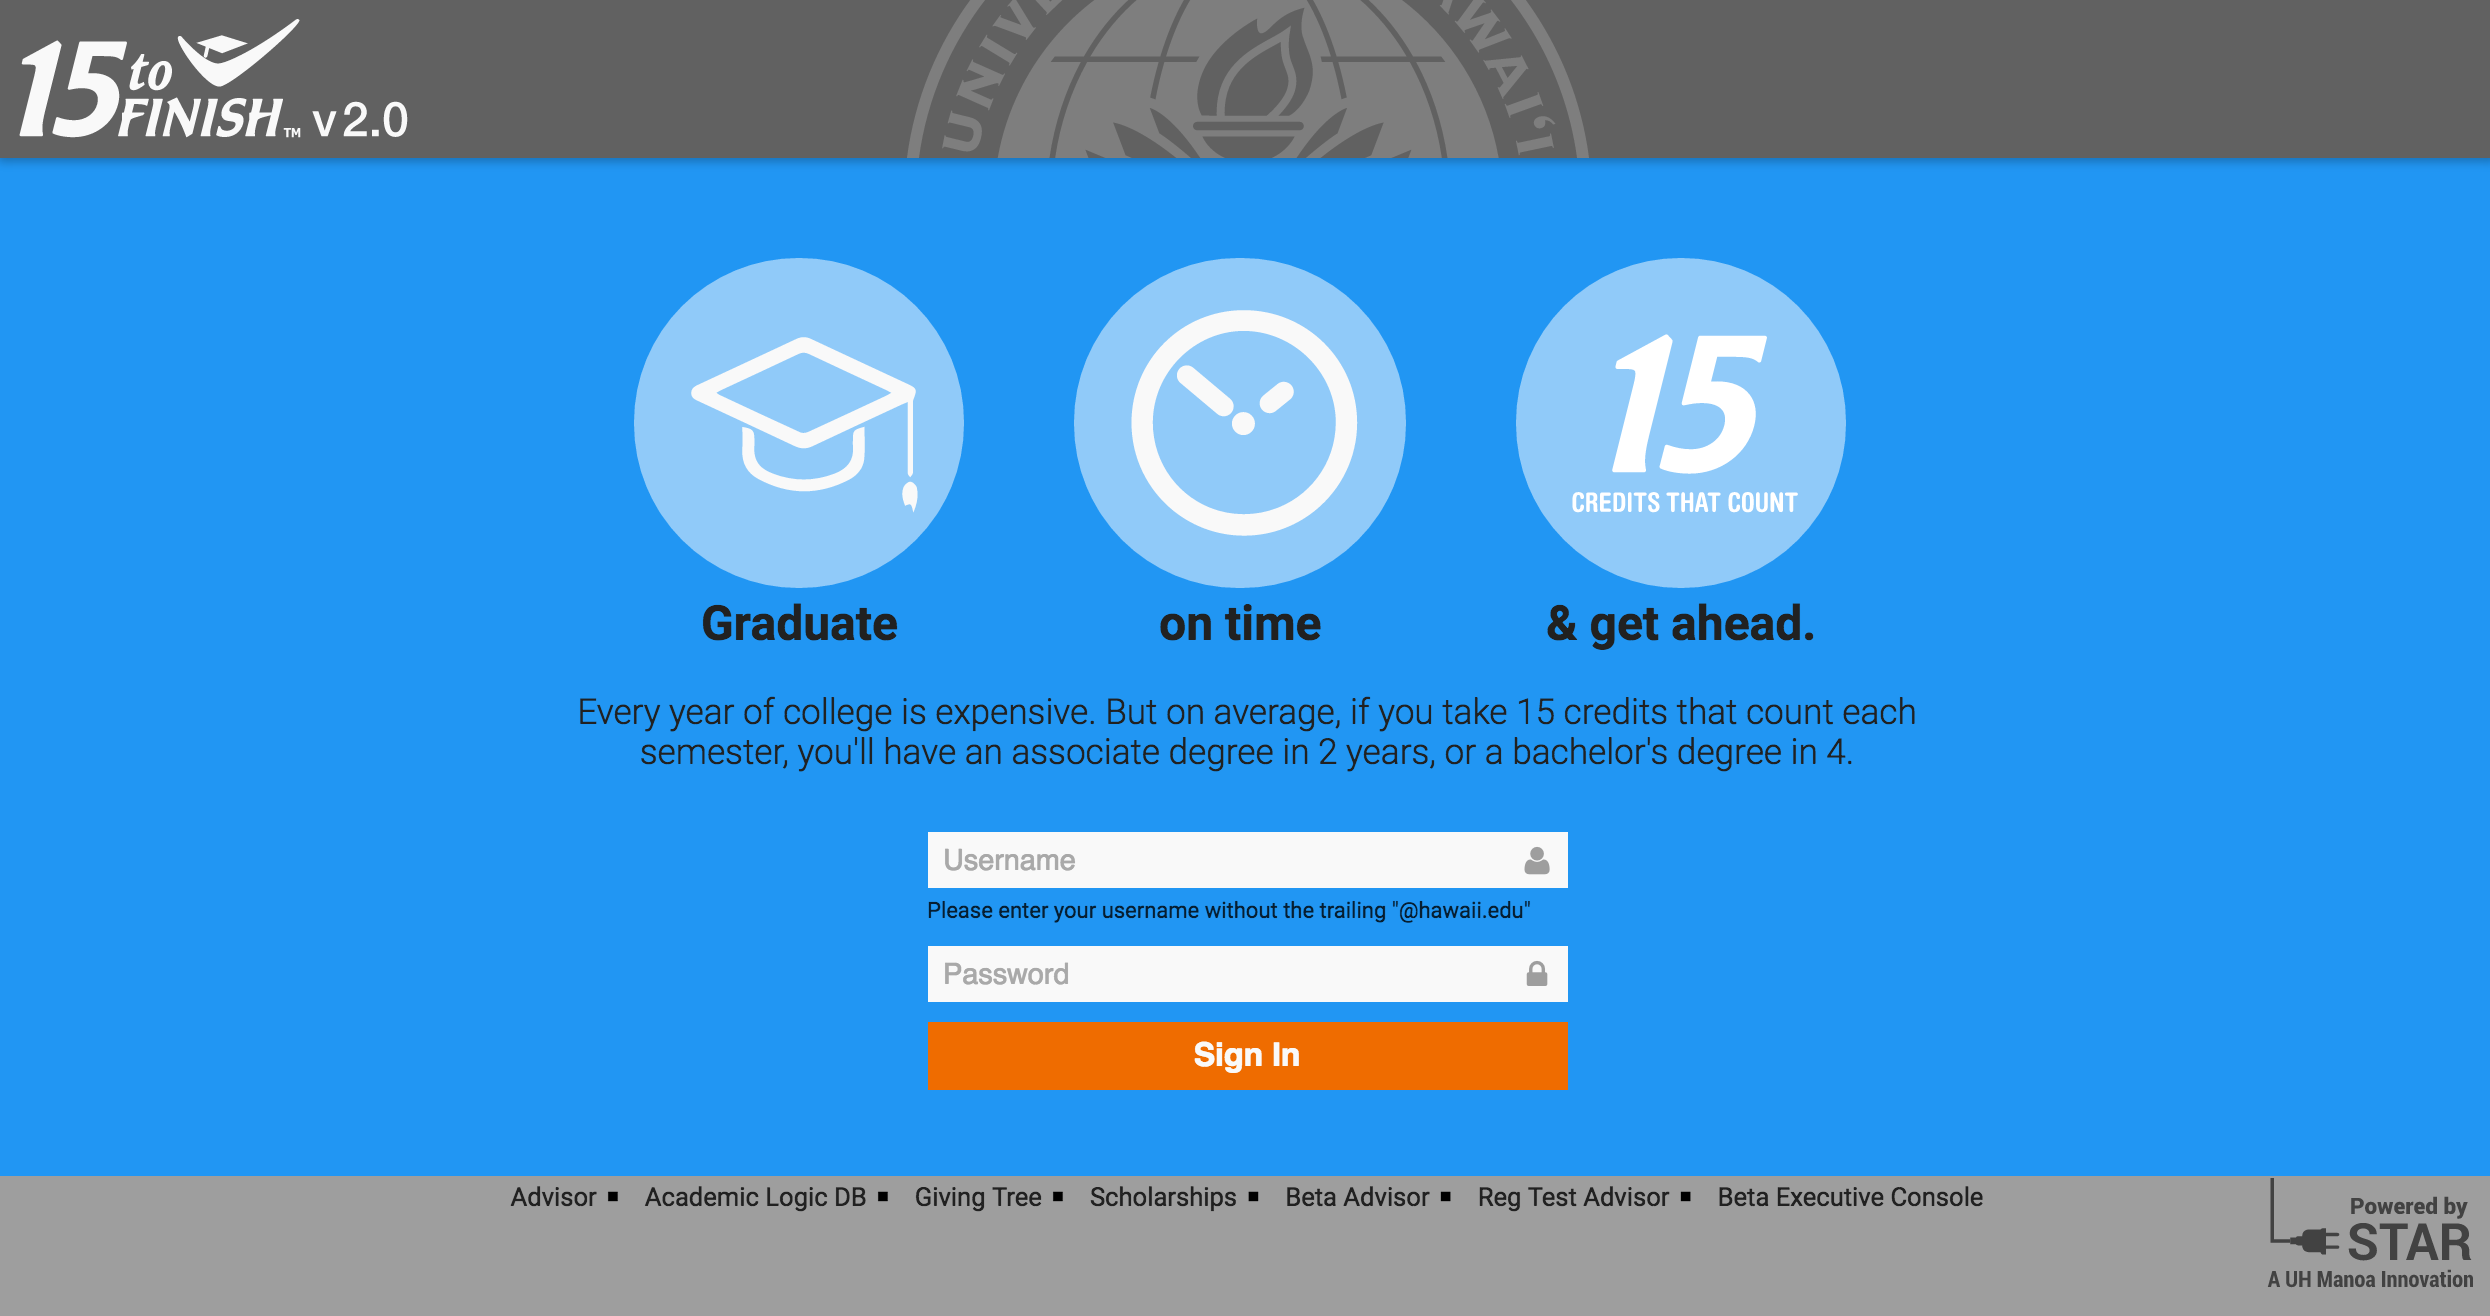
\includegraphics[width=1.0\textwidth]{star_home}
\caption{STAR homepage. \textit{Source: www.star.hawaii.edu}}
\end{figure}
\subsection{STAR}
STAR is the degree planning system currently used by the University of Hawaii. As of September 2016, the student interface provides five main capabilities: Academic Essentials, Graduation Pathway, What If Journey, Transcripts, and Scholarships. 

\begin{figure}[h]
\centering
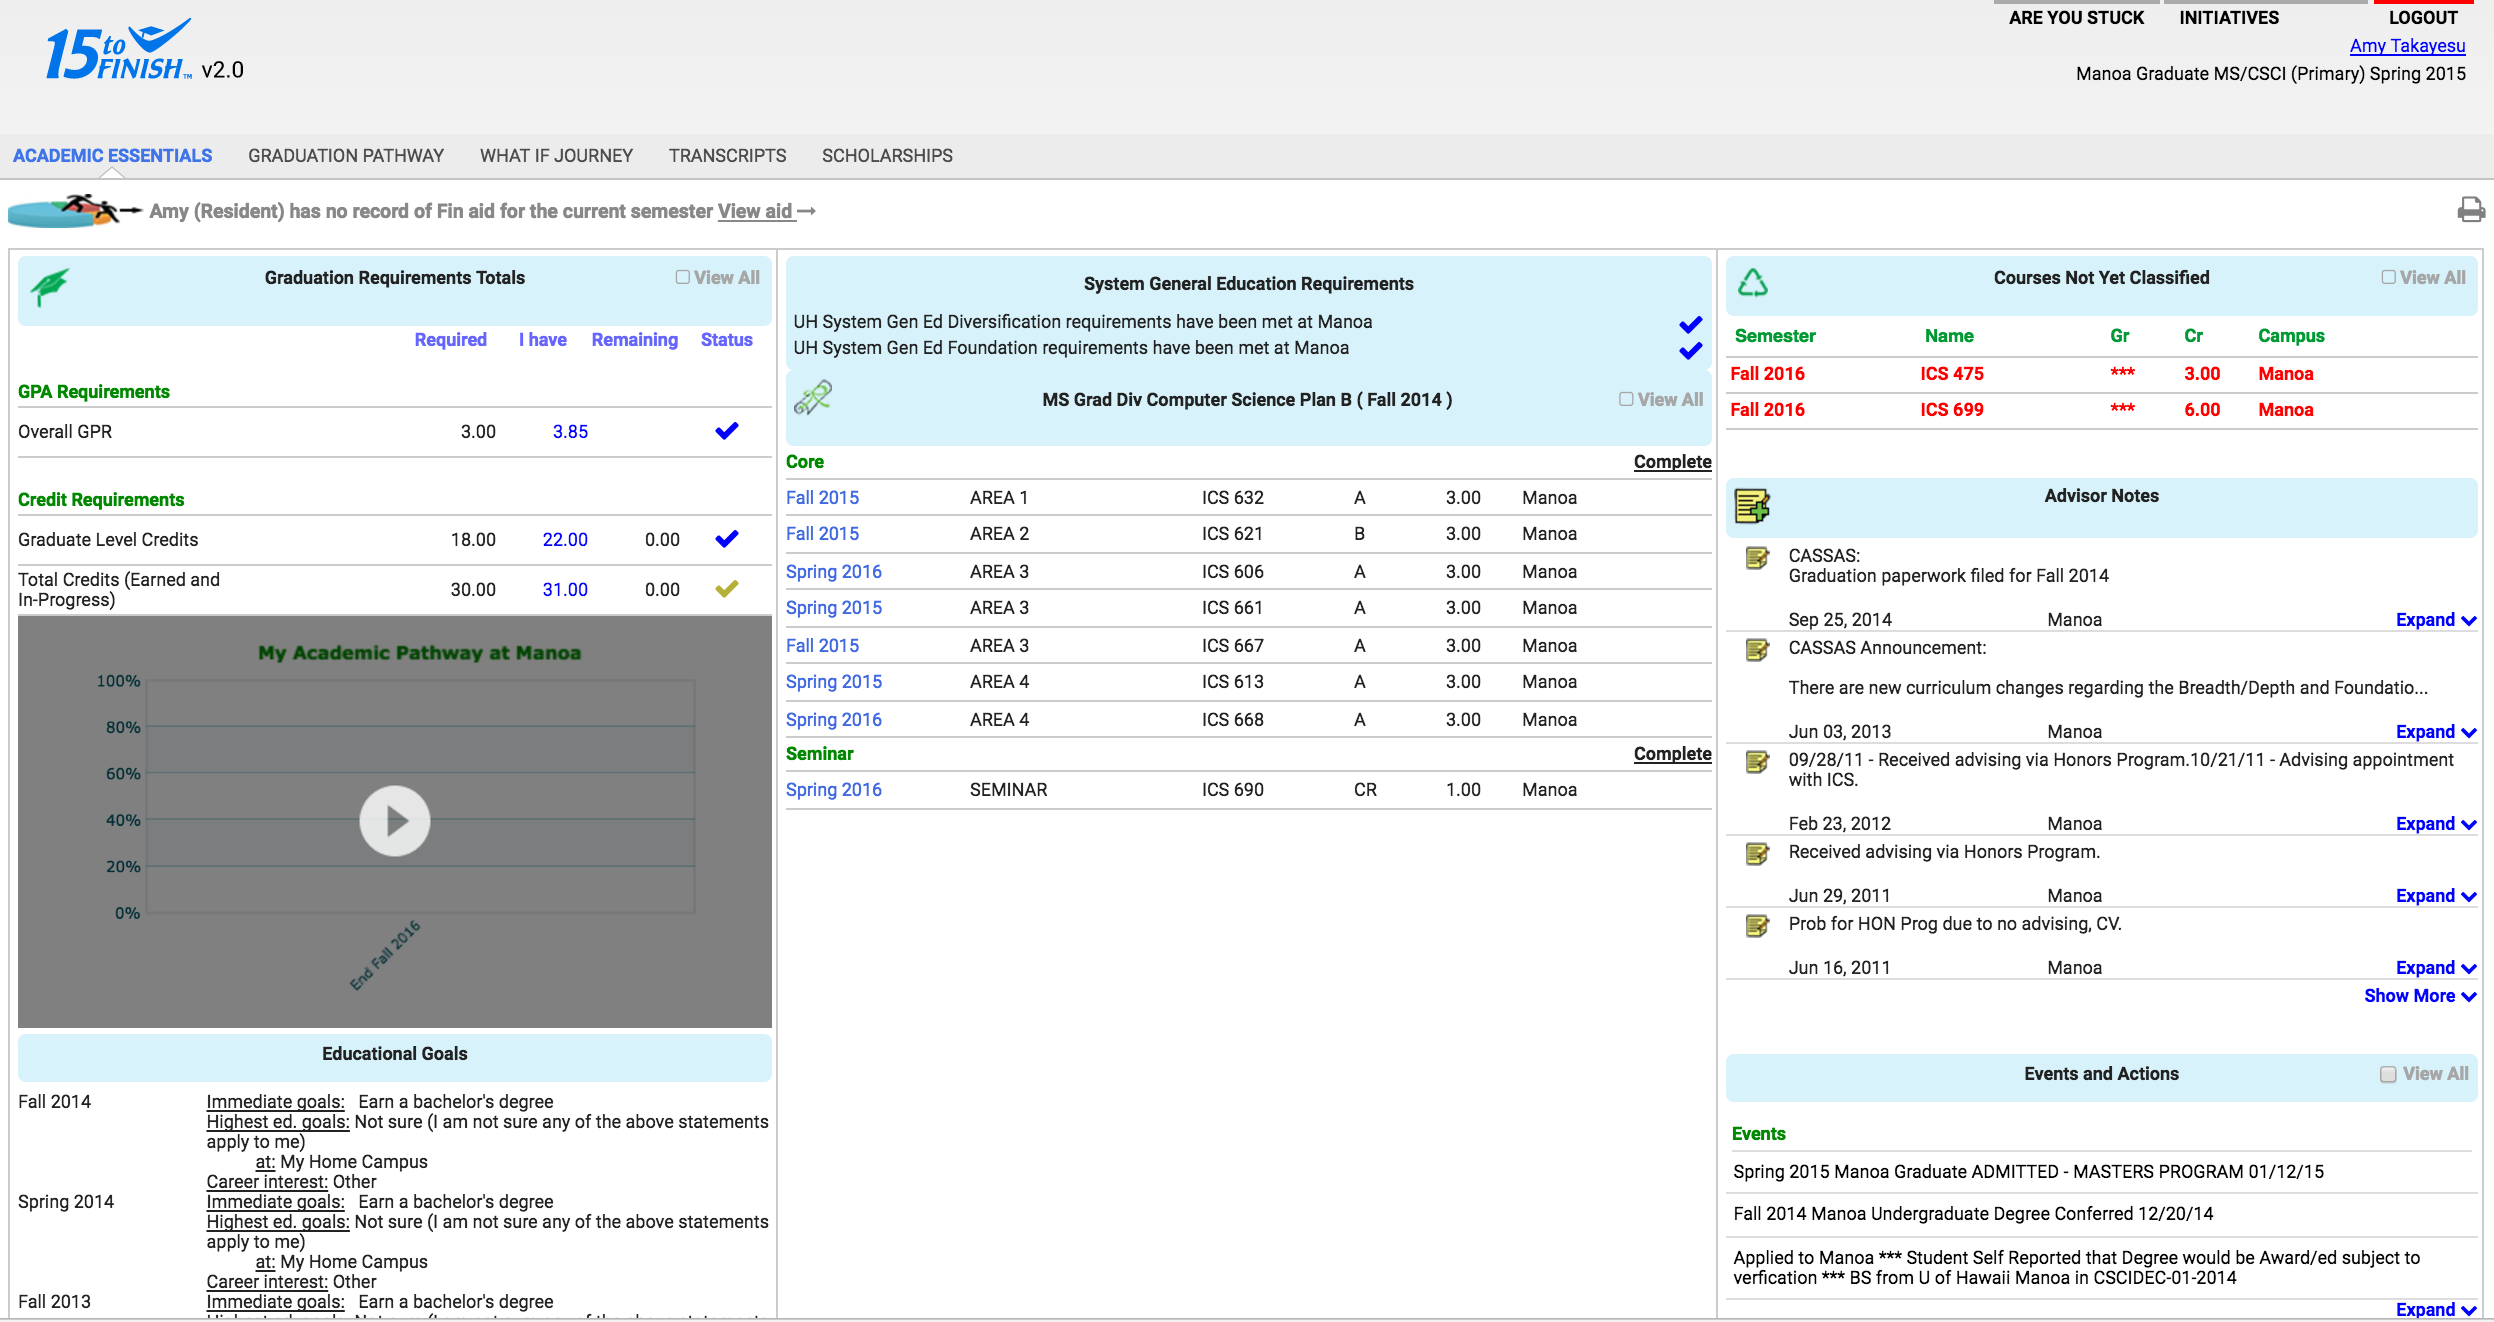
\includegraphics[width=1.0\textwidth]{star_edgoals}
\caption{STAR Academic Essentials page. \textit{Source: www.star.hawaii.edu}}
\end{figure}
\subsubsection{Academic Essentials}
This interface provides information about the student's academic progress, and compares it to the student's academic requirements to show how close the student currently is to graduation. This information includes credit totals, grades, and required courses. This interface also includes a section for ``Advisor Notes", which is filled out during advising sessions. There is another section for ``Events and Actions" which lists important student academic events such as college applications, admittance, and graduation, and student academic actions such as Deans List award. A third section is called ``Educational Goals", which provides the student's ``immediate goals" and ``highest ed goals" on a semester-by-semester basis. This information is provided by the student through occasional assessments upon log-in to STAR. The top of the page also has a section for students with financial aid.

\begin{figure}[h]
\centering
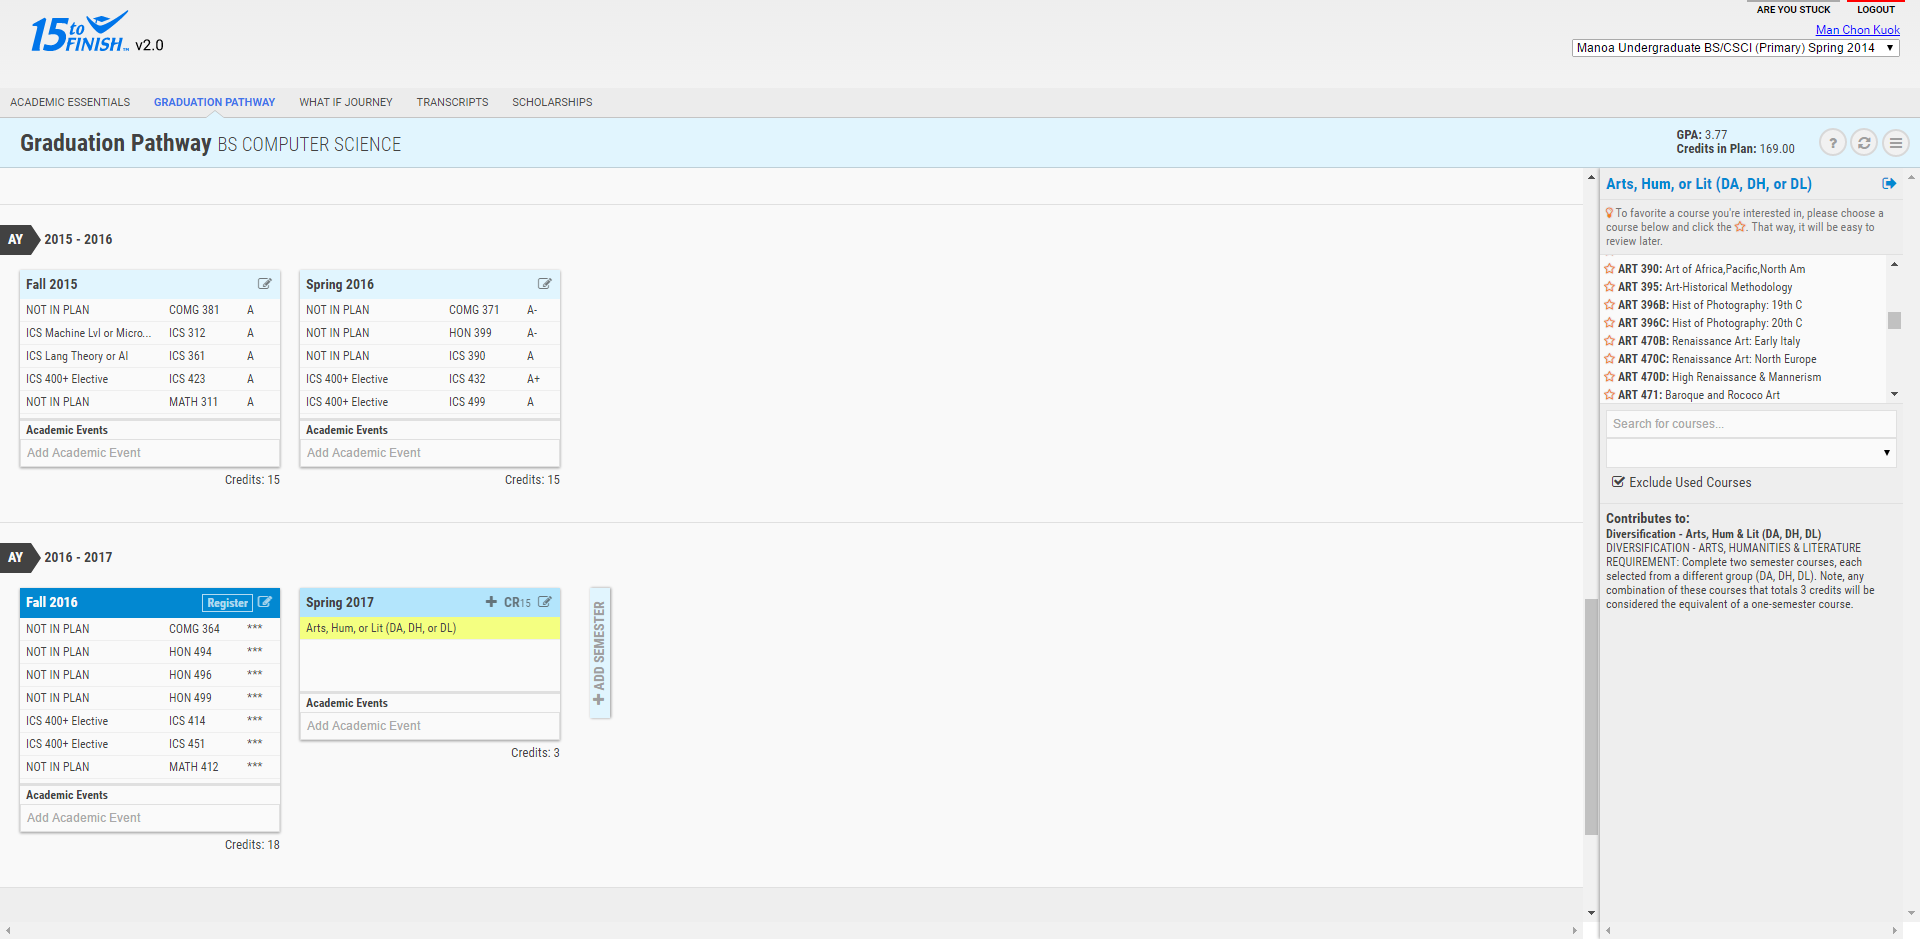
\includegraphics[width=1.0\textwidth]{star_pathway}
\caption{STAR Academic Graduation Pathway page.\textit{Source: www.star.hawaii.edu}}
\end{figure}

\subsubsection{Graduation Pathway}
This interface is provided for certain programs or exploratory or pre-major students. It shows the course information for the courses that the student has taken previously and is currently enrolled in, and shows which requirements each course fulfills. It also shows future semesters and suggests future types of classes that the student should enroll in, in order to fulfill their major requirements. This interface does not suggest specific classes, but only lists the requirement that the class will need to fulfill. 

\begin{figure}[h]
\centering
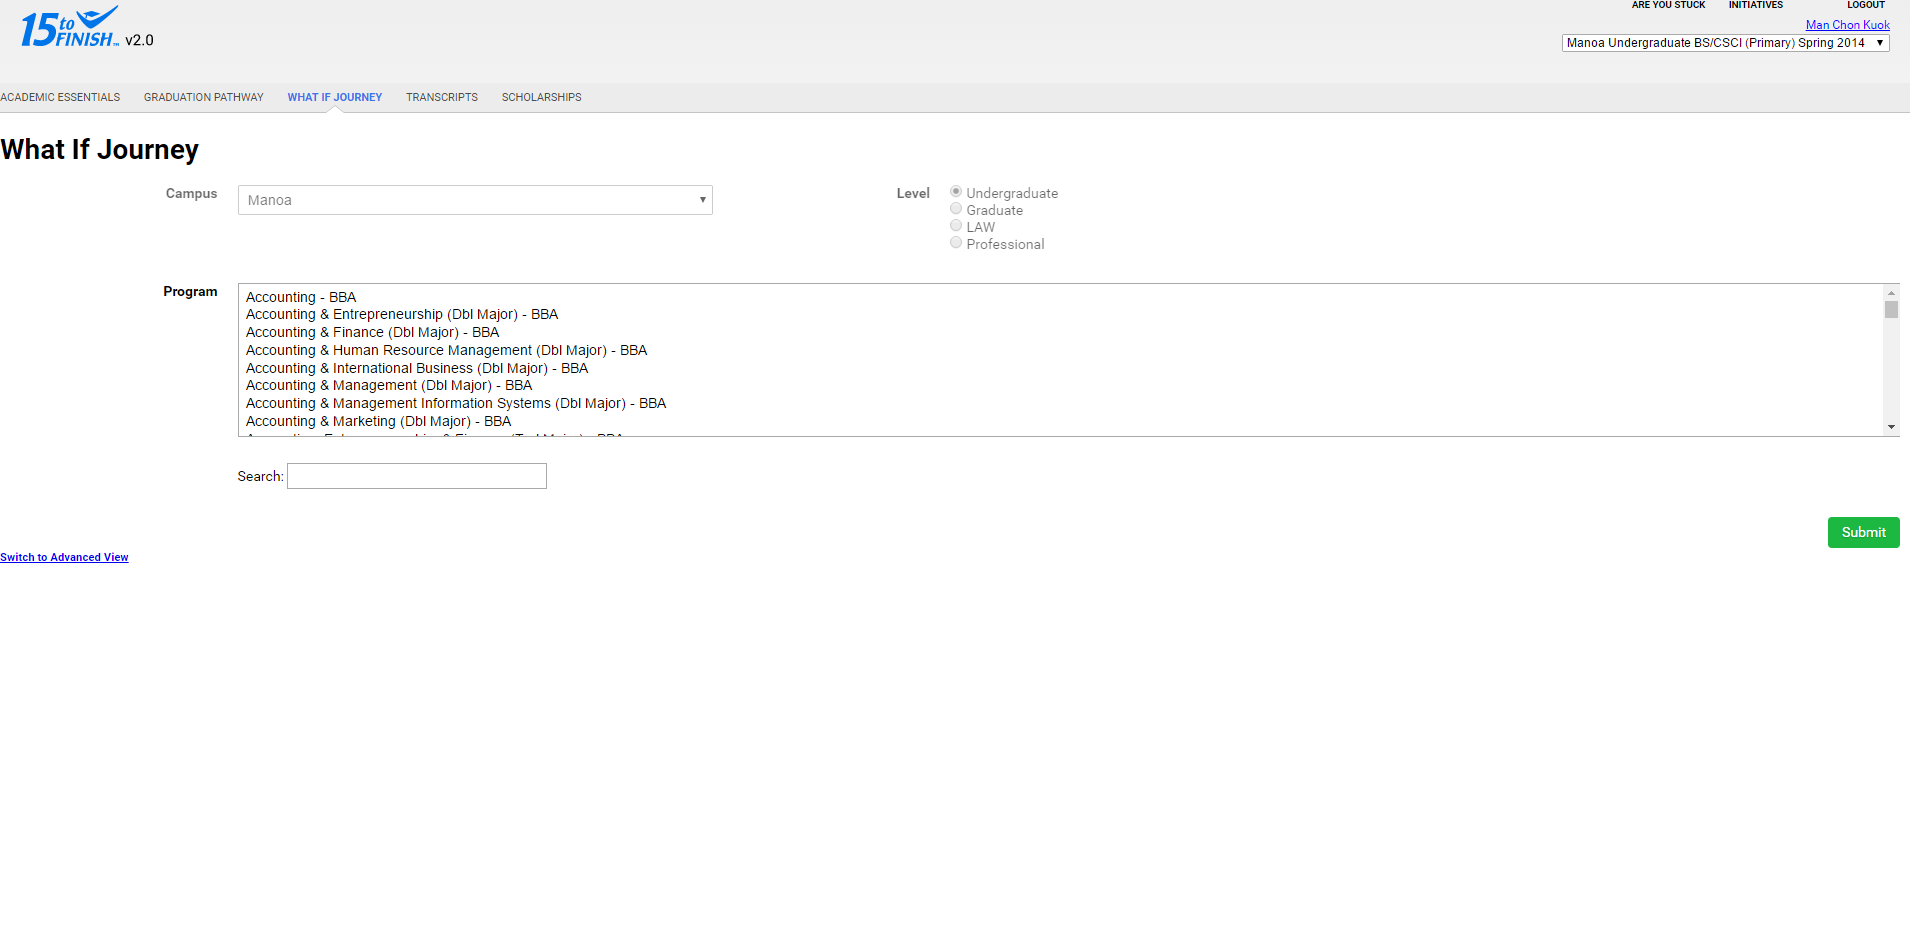
\includegraphics[width=1.0\textwidth]{star_whatif}
\caption{STAR What If page. \textit{Source: www.star.hawaii.edu}}
\end{figure}

\subsubsection{What If Journey}
This interface is provided for undergraduates at UH Manoa. It allows students to choose a different major than the one they are currently in. The page then reloads to show the STAR homepage, altered to show the requirements of the chosen major. This shows students where they would be in the program if they were to switch majors.

\begin{figure}[h]
\centering
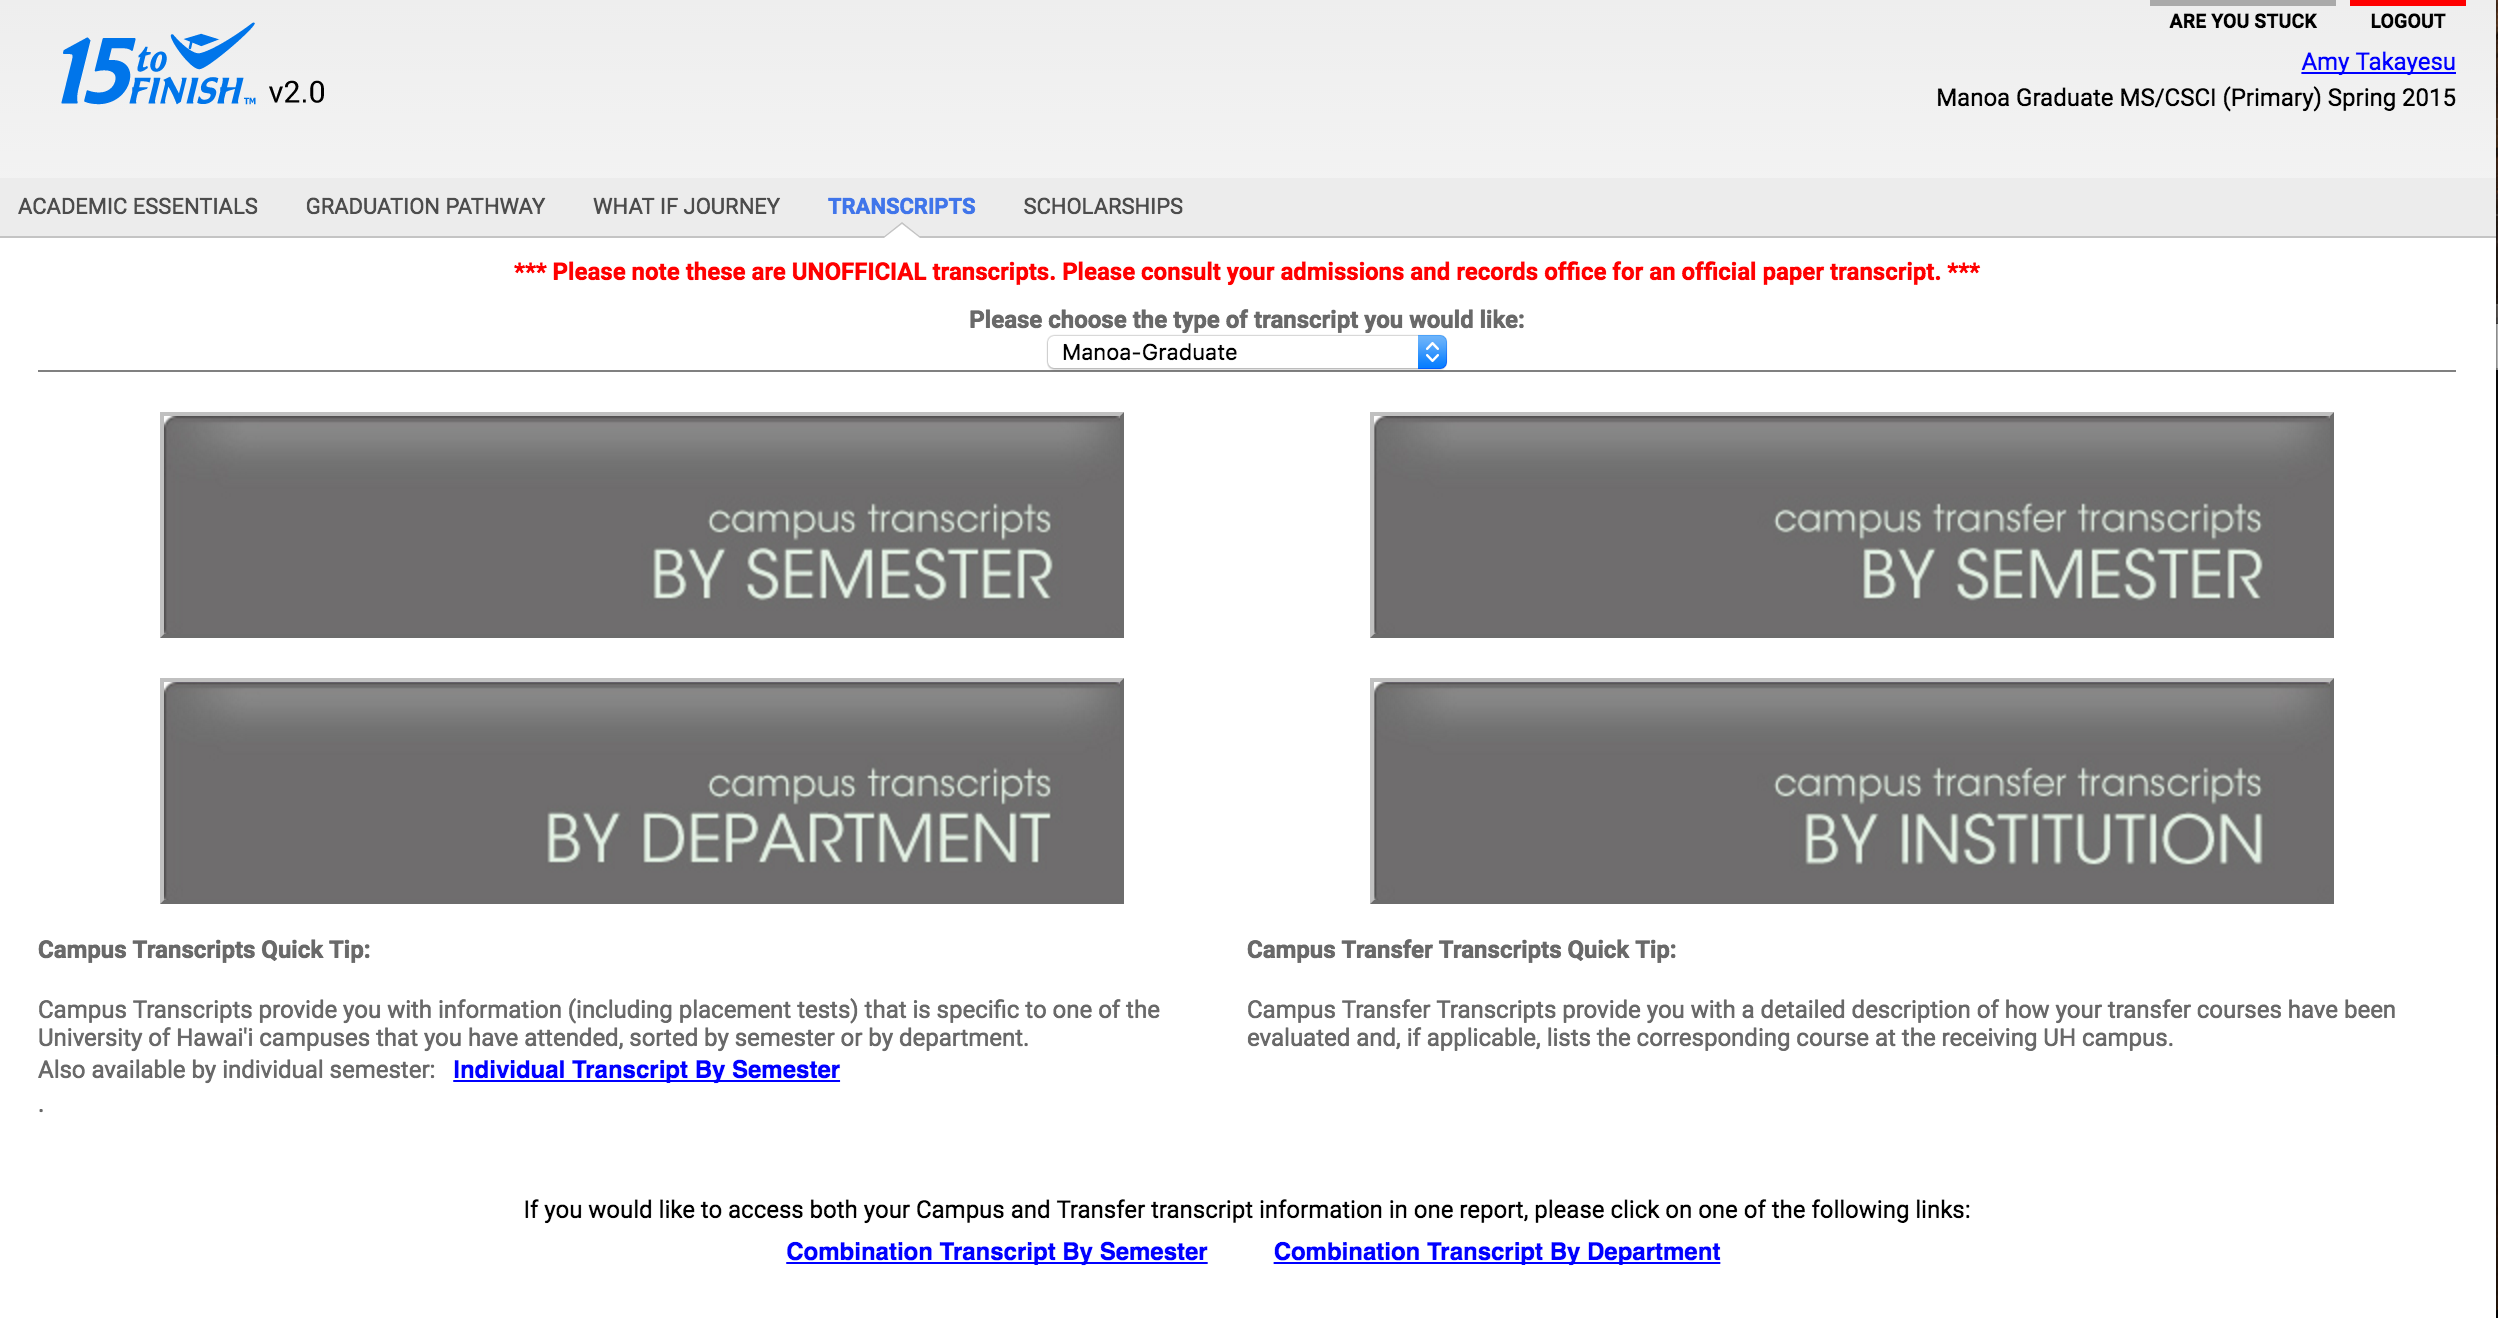
\includegraphics[width=1.0\textwidth]{star_trans}
\caption{STAR Transcripts page. \textit{Source: www.star.hawaii.edu}}
\end{figure}

\subsubsection{Transcripts}
This interface allows students to access their campus transcripts by semester and by department. It also allows transfer students to access their transfer transcripts by semester and by institution. 
\begin{figure}[h]
\centering
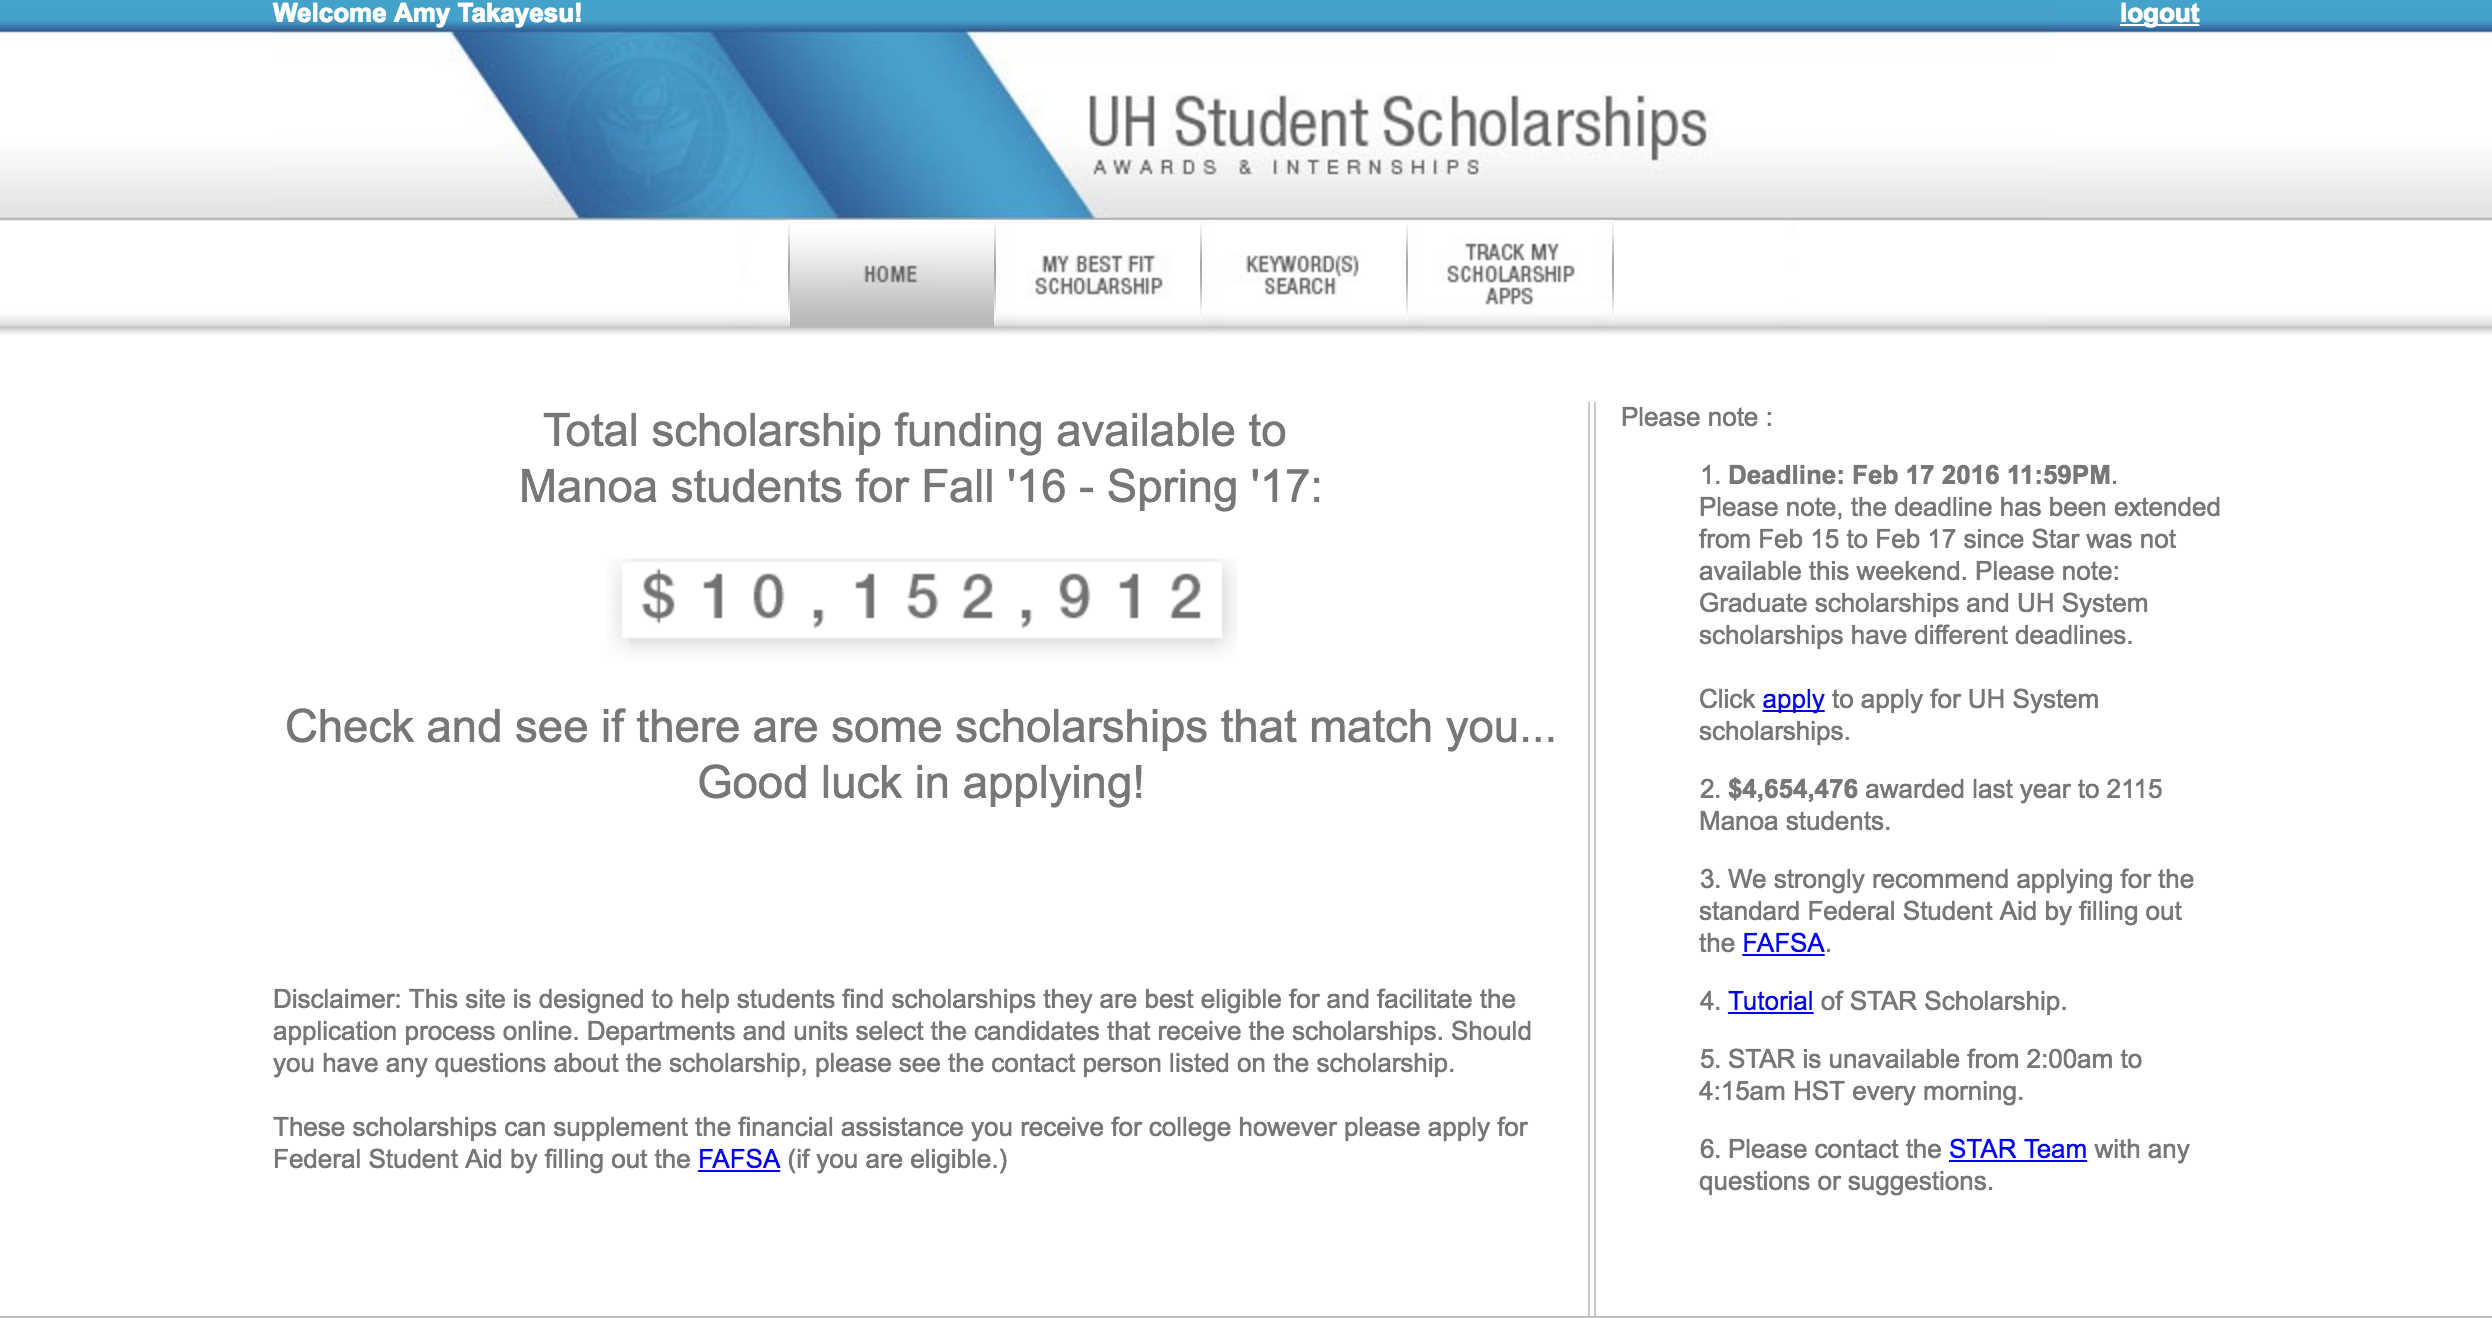
\includegraphics[width=1.0\textwidth]{star_scholar2}
\caption{STAR Academic Scholarship Home page. \textit{Source: www.star.hawaii.edu}}
\end{figure}
\begin{figure}[h]
\centering
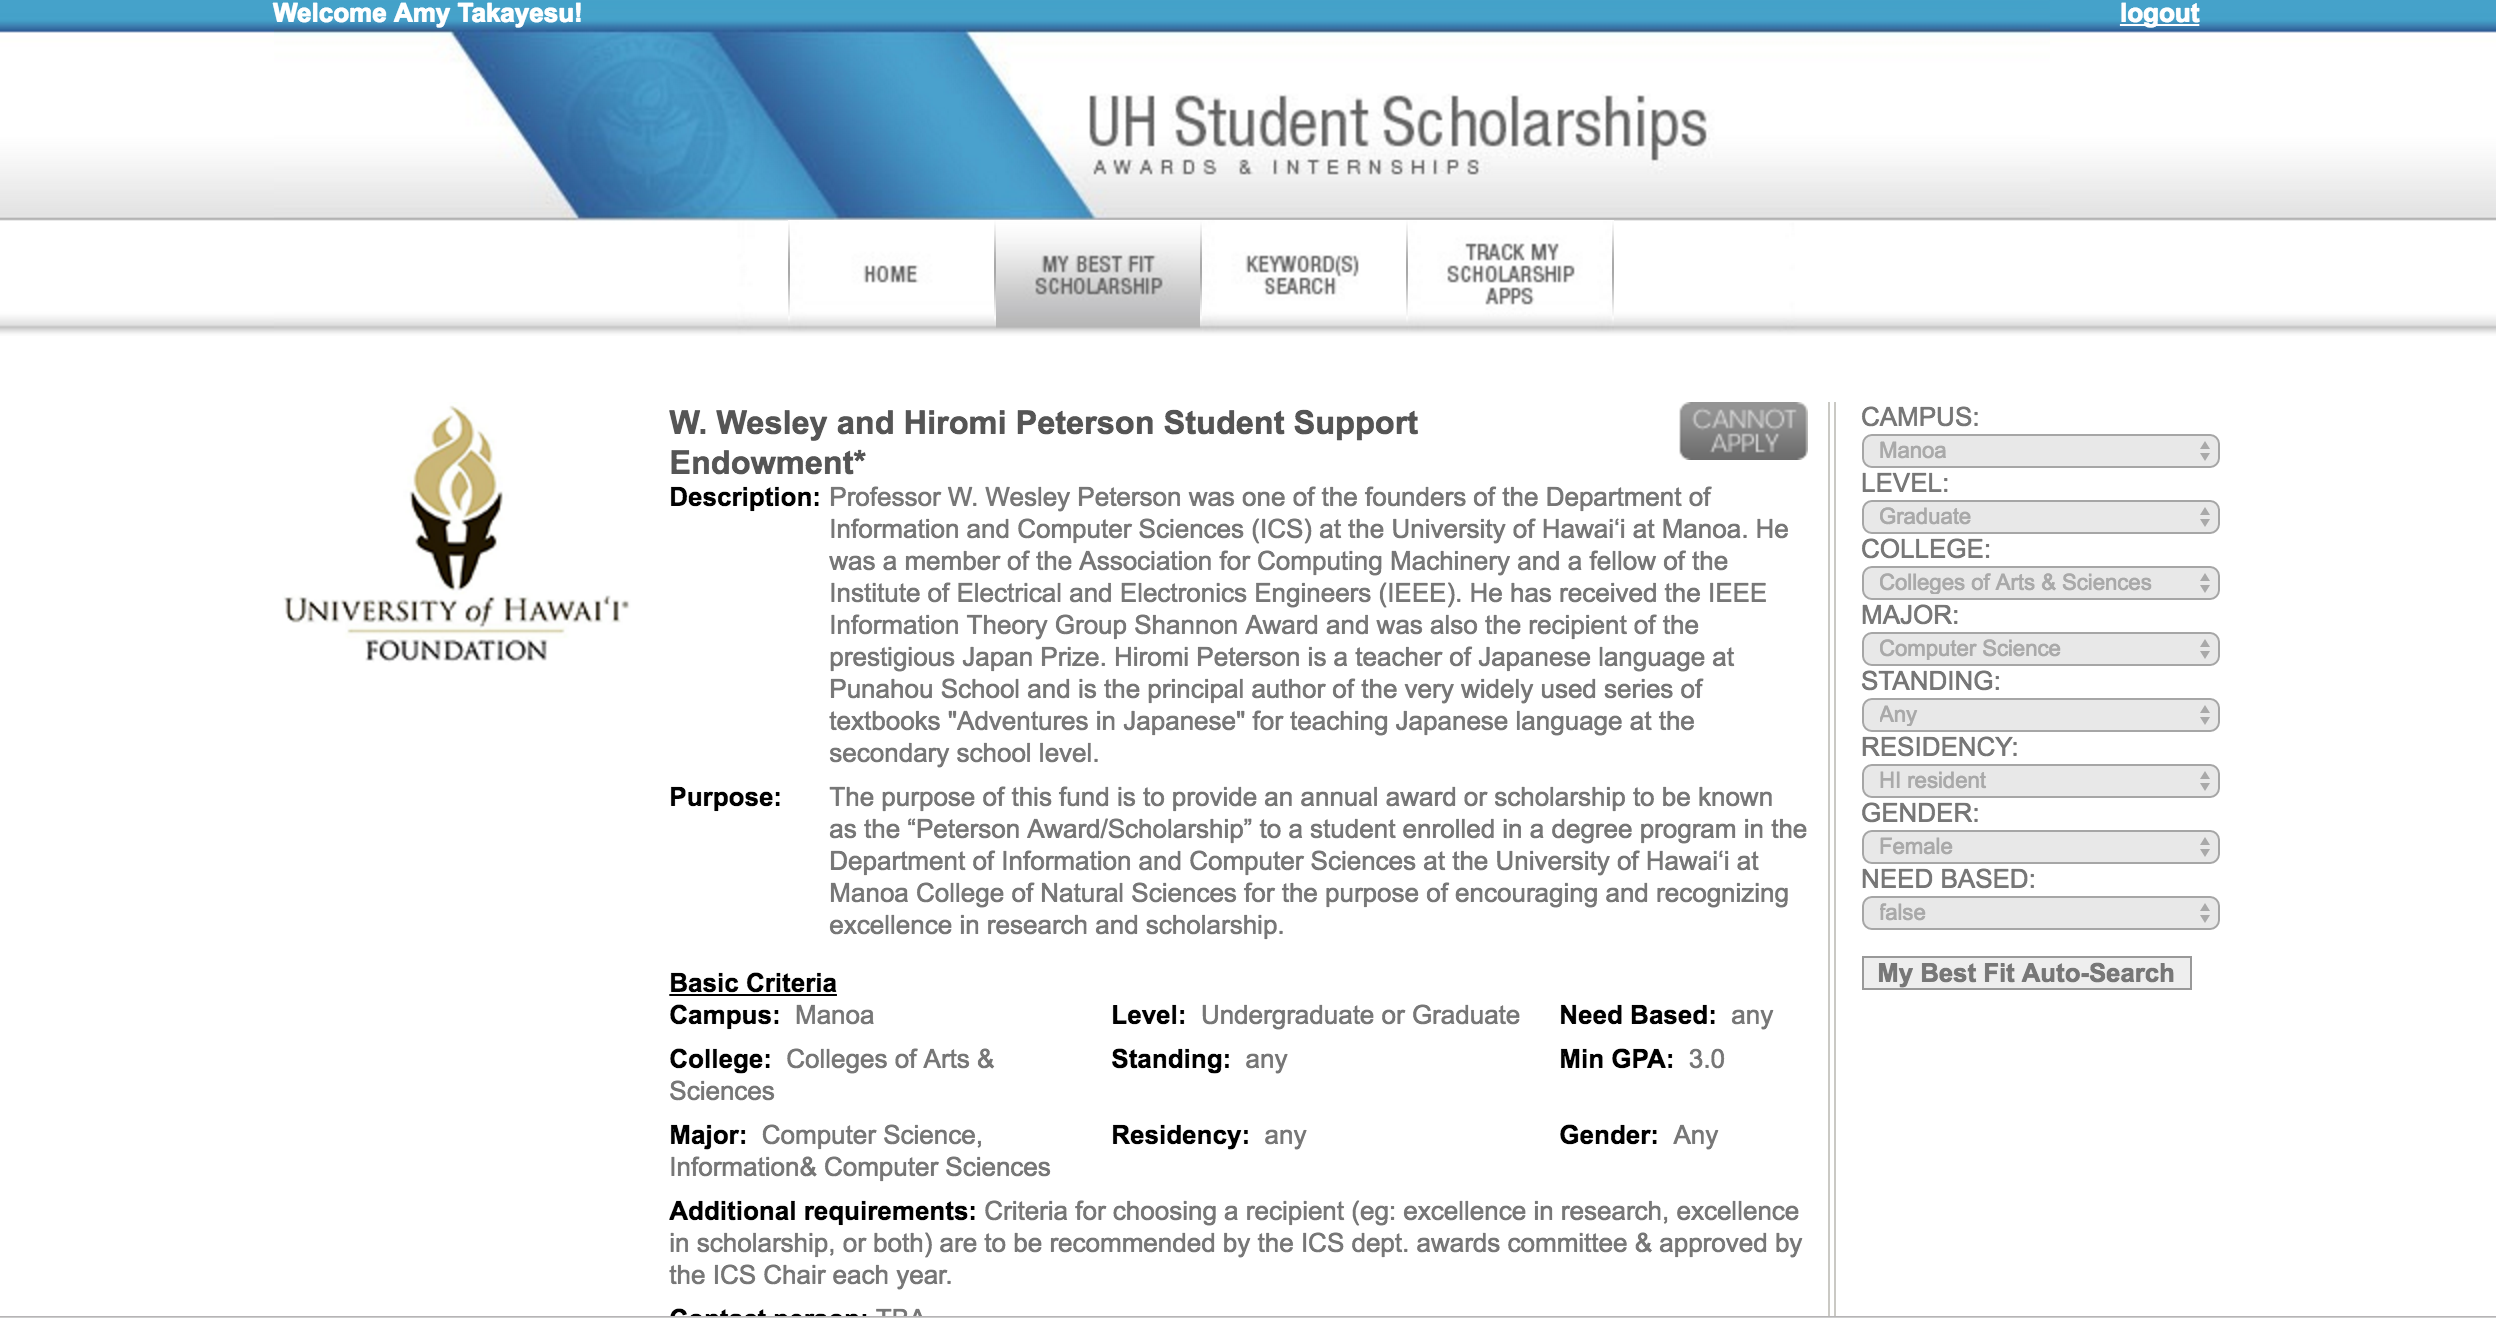
\includegraphics[width=1.0\textwidth]{star_scholar3}
\caption{STAR Academic Scholarship Best Fit page. \textit{Source: www.star.hawaii.edu}}
\end{figure}
\begin{figure}[h]
\centering
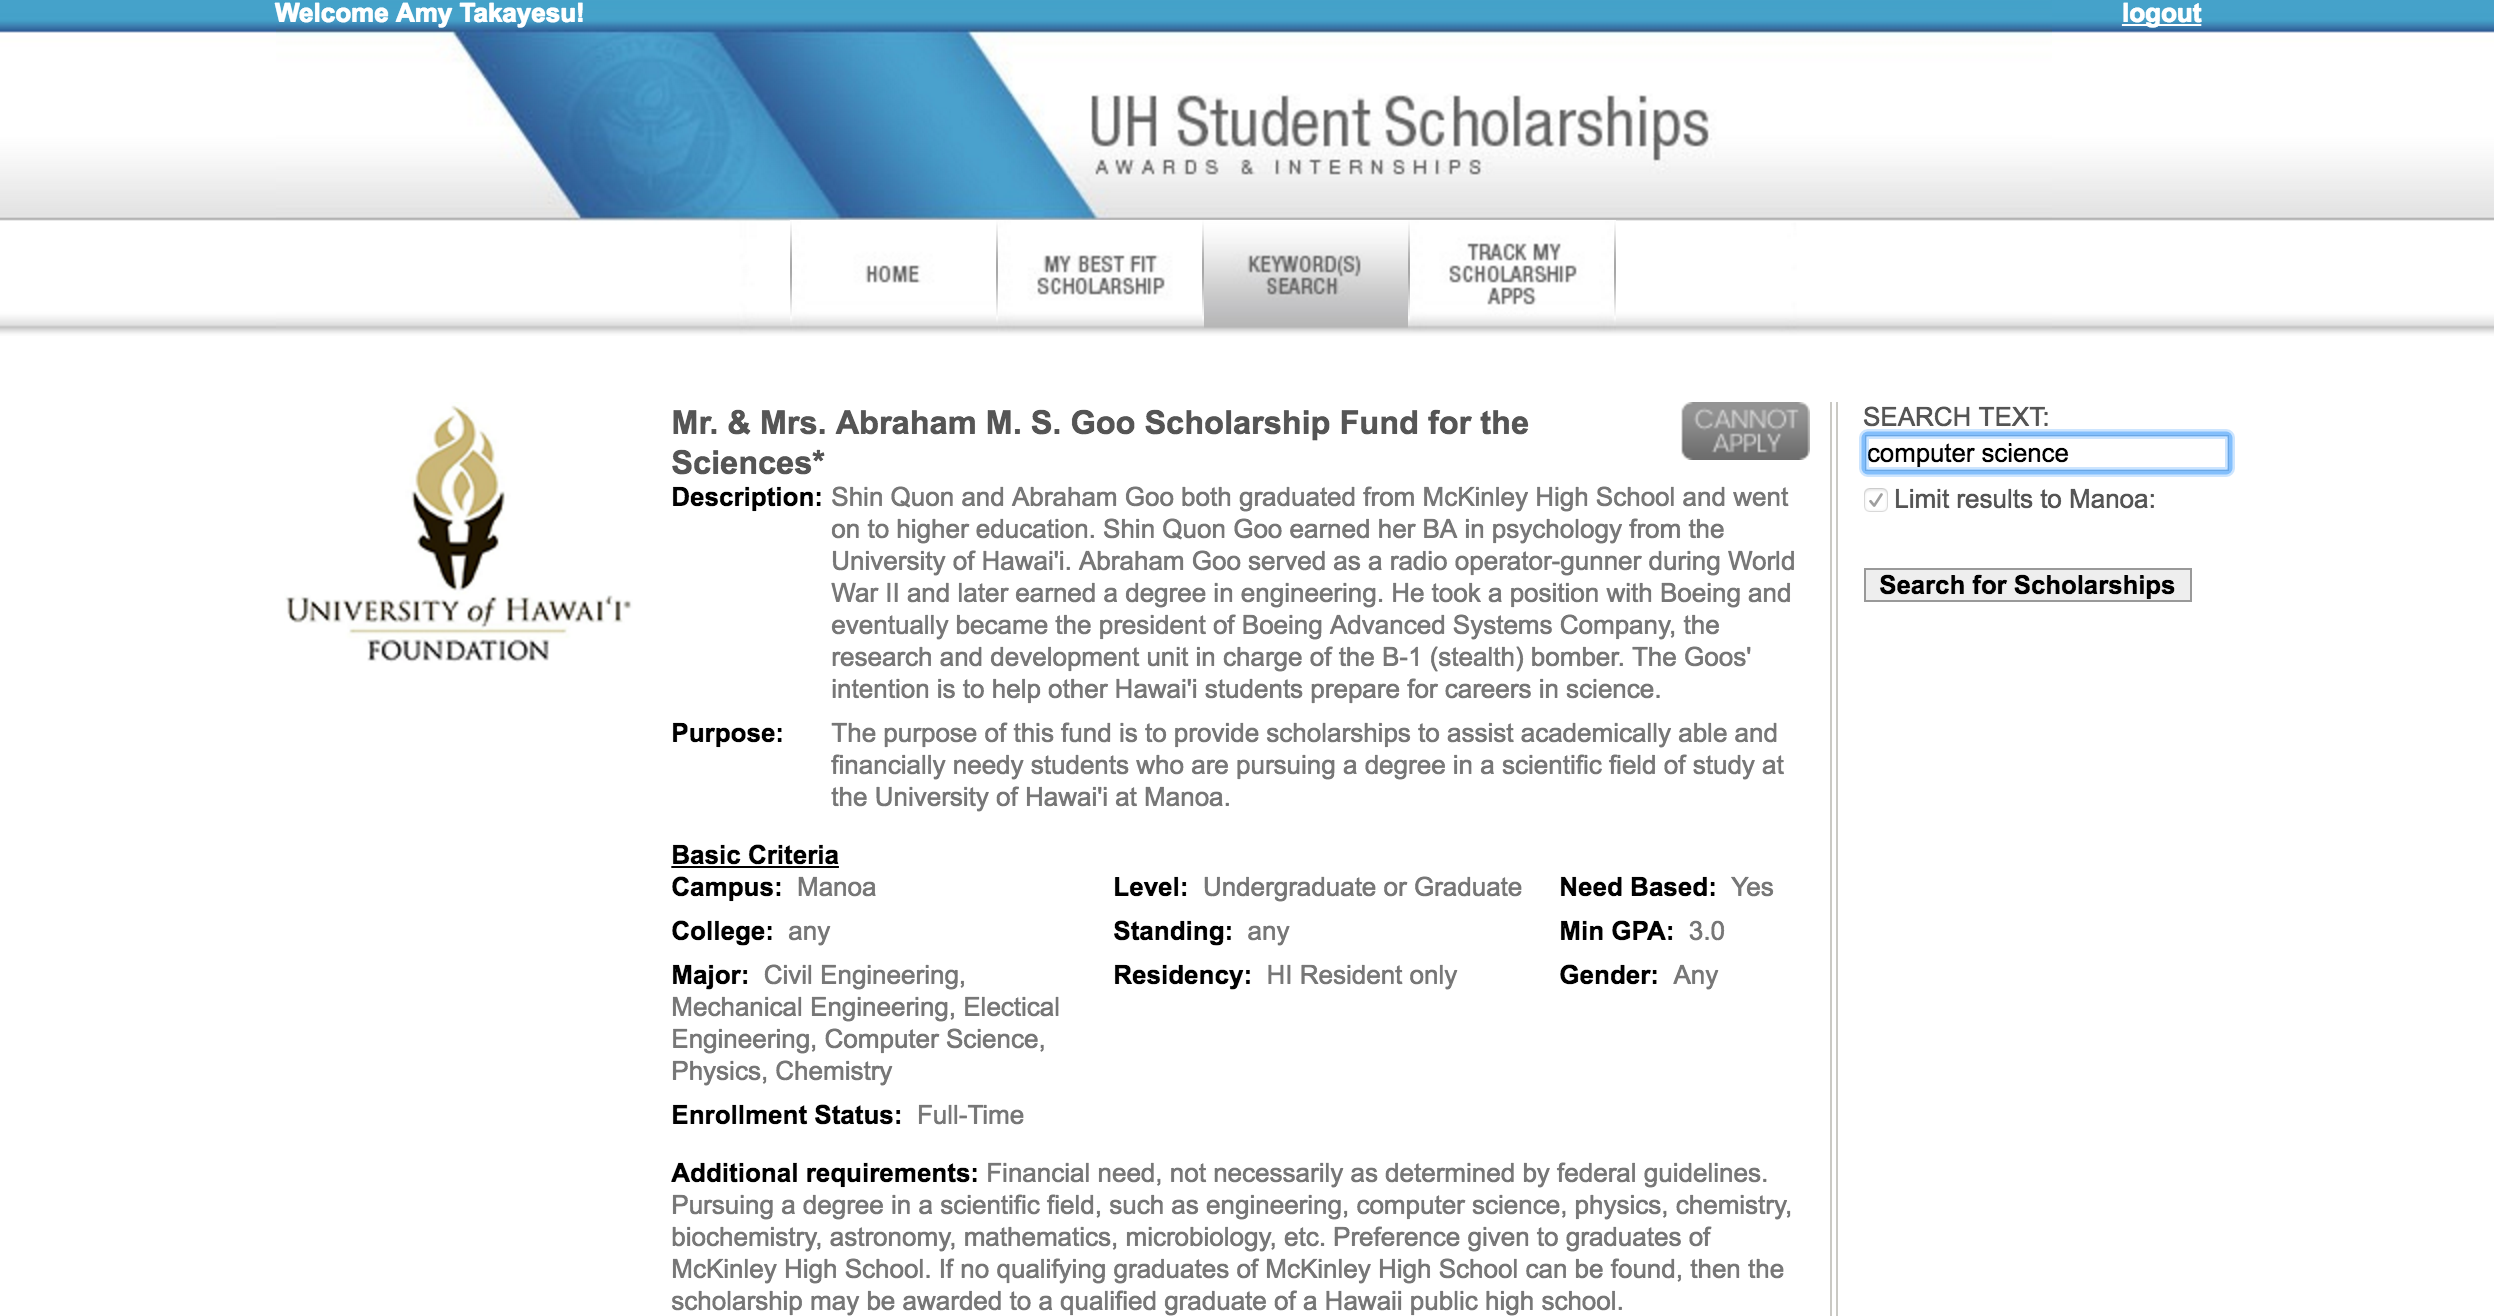
\includegraphics[width=1.0\textwidth]{star_scholar4}
\caption{STAR Academic Scholarship Keyword Search page. \textit{Source: www.star.hawaii.edu}}
\end{figure}
\subsubsection{Scholarships}
This interface allows students to find scholarships by either using a keyword search or by selecting the ``My Best Fit Scholarship" tab, which presumably gathers student academic data and compares it with scholarship data to find matches.

\subsubsection{STAR and Academic/Professional/Social Engagement}
STAR is the all-in-one place for UH students to check on their progress in general education and major courses, University status in terms of enrollment and tuition payment, and their official transcripts. Since STAR is designed to fit the general academic needs of all students at UH, it is unrealistic to expect STAR to provide specialized and detailed support for each department. Each department is different in terms of courses and requirements, and STAR does not offer any features that go into depth in each individual department's idiosyncrasies. To get more detailed information about major requirements, students must access separate department websites or contact the department's academic adviser. 
In features such as Academic Essentials, Graduation Pathway, and Scholarships, STAR only offers baseline information. For instance, in Academic Essentials, STAR focuses on the student's broad academic goals (i.e. graduation date and highest degree goal) rather than their arguably more helpful and specific major-related goals. In Graduation Pathway, STAR notifies students which course categories they are missing, but does not suggest the specific classes that they are missing. In Scholarships, STAR lists relevant scholarships but does not provide detailed information about how to apply or how to prepare for them. Although STAR succeeds at being a University-wide, cross-departmental degree planner system, it lacks the detailed department-specific support that is crucial for a student's success and growth within his/her major. 

\begin{figure}[h]
\centering
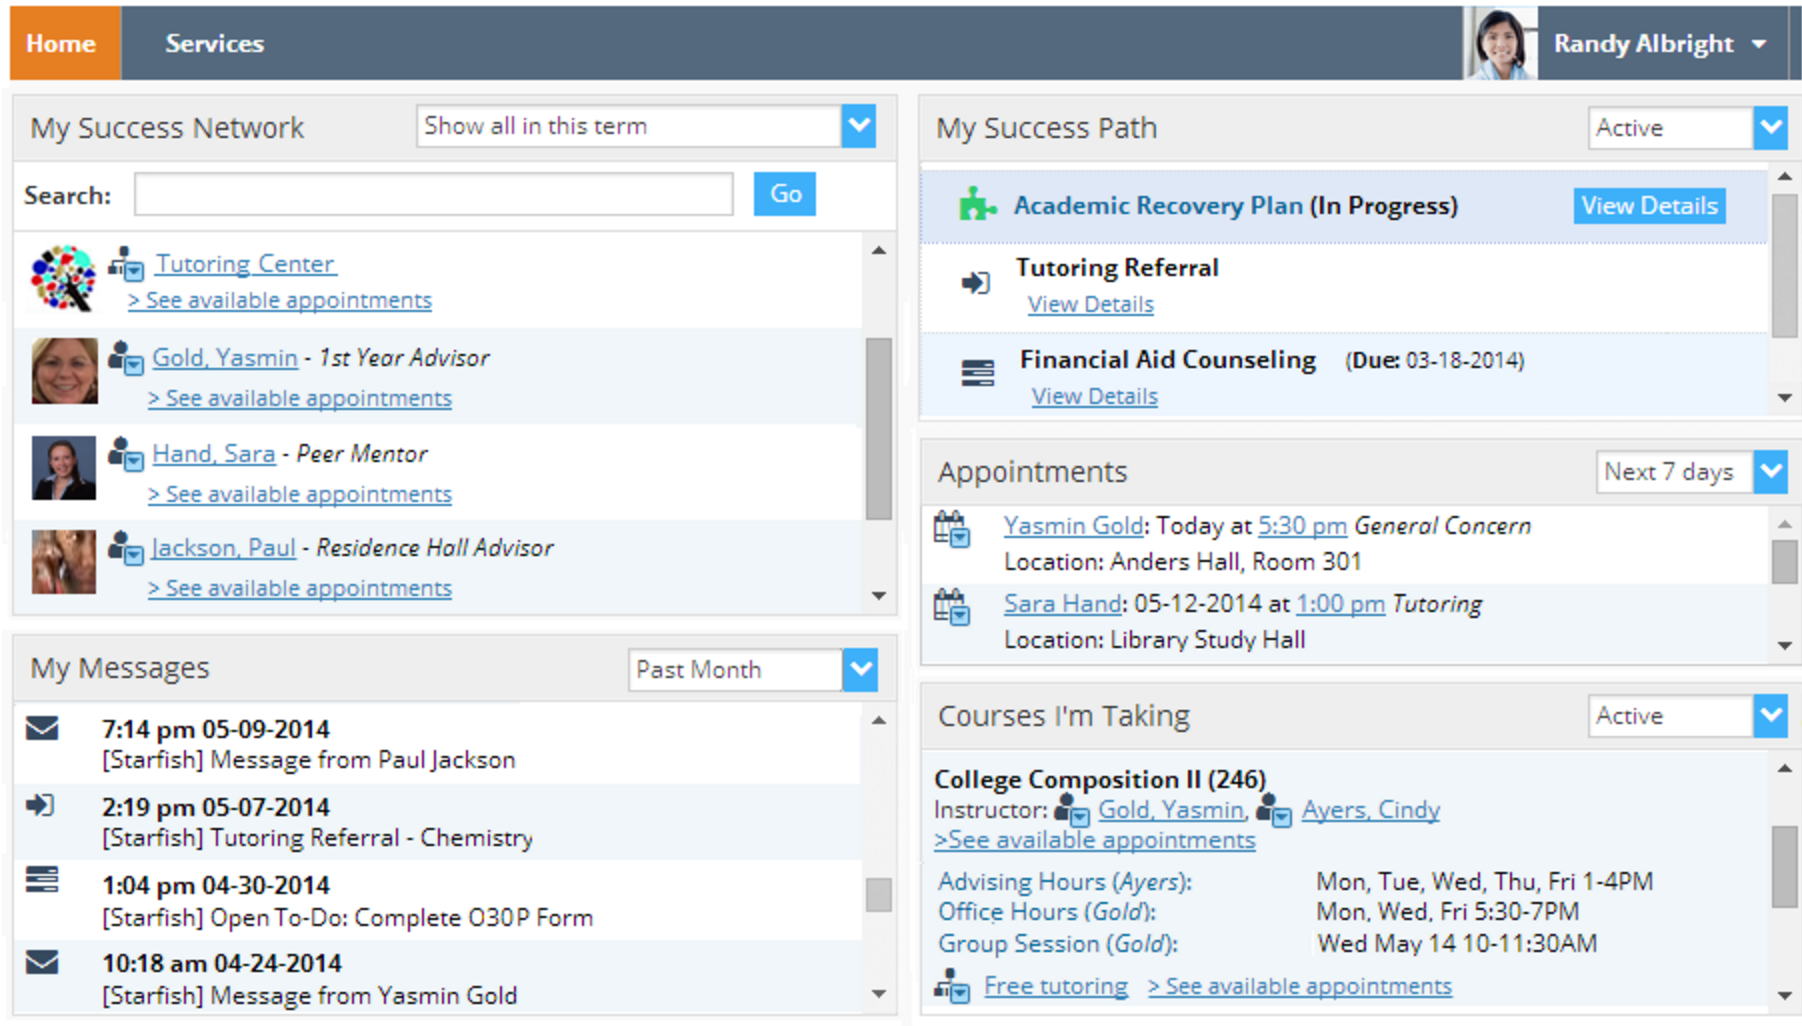
\includegraphics[width=1.0\textwidth]{starfish_connect}
\caption{Example Starfish Connect page. \textit{Source: Starfish CONNECT gallery}}
\end{figure}
\subsection{Starfish by Hobsons}
The slogan for Hobsons is ``Education Advances: Imagine a world where all students find their best fit." Hobsons offers a wide range of educational solutions, ranging from students K-12 to college students. Starfish by Hobsons is one of their platforms which focuses on success, support, and retention initiatives, and engaging students more effectively with the campus community. There are three main parts of the Starfish Enterprise Success System: Early Alert, Connect, and Degree Planner.
\subsubsection{Early Alert}
Early Alert is a early warning and student tracking model which mines student performance data from existing technologies at the particular institution to detect at-risk students. These students are detected early enough, such as at the first sign of a problem, so that there is enough time to make a difference. There is a type of reward system called Kudo (a positive feedback note), which is used to encourage students and reward them for improvement or good work. 
\subsubsection{Connect}
Connect is an online appointment scheduling and case management system. This system promotes communication between students and their advisers, instructors, and tutors by means of in person meetings, phone calls, or virtual meetings. Connect includes a kiosk to allow easily scheduled walk-in meetings. These kiosks can help staff to manage a student queue and also allows students to check wait times remotely, which can save a lot of time and frustration. Connect also includes a road map for each student, which documents the steps a student must take to achieve his or her goals. This map is created by an adviser and is visible to all members of the student's support network. 
\subsubsection{Degree Planner}
Degree Planner provides academic templates which advisers can use to easily edit to adjust to a particular student's needs. It also focuses on students' constantly changing goals and ability to adjust the student's plan to accommodate these goals. When a student deviates from their given plan, the student's adviser is notified so that they can plan a meeting with the student to check on their status and re-identify their goals. 

\subsubsection{Starfish by Hobsons and Academic/Professional/Social Engagement}
Starfish by Hobsons provides integrated systems that can keep track of students and keep students on track. It's integration into different departments and customization of more specific goals fulfills the academic goals of RadGrad more than STAR. However, this system is concerned only with academics and does not take other factors into consideration such as internships, outside work and projects, and other extracurricular activities. While a student may seem to be on track based off their academic record, there are other factors that come into play when it comes to ``staying on track." Traditionally, an ``on track" student may have completed all of the coursework within 4 years with at least a 3.0 GPA. However, what if ``on track" were redefined to be much more complex, and include other factors outside of coursework? Although these factors may not technically be requirements to graduate, they may be highly recommended, and a system that could help encourage students to pursue these other factors, without them being technically required, would create a different class of graduates entirely. 

\subsection{College Scheduler}
The College Scheduler company has two products: Schedule Planner and Pathway Planner. The Schedule Planner focuses on optimizing the way students can plan their schedules, and the Pathway Planner focuses on optimizing the way students progress towards graduation.

\begin{figure}[h]
\centering
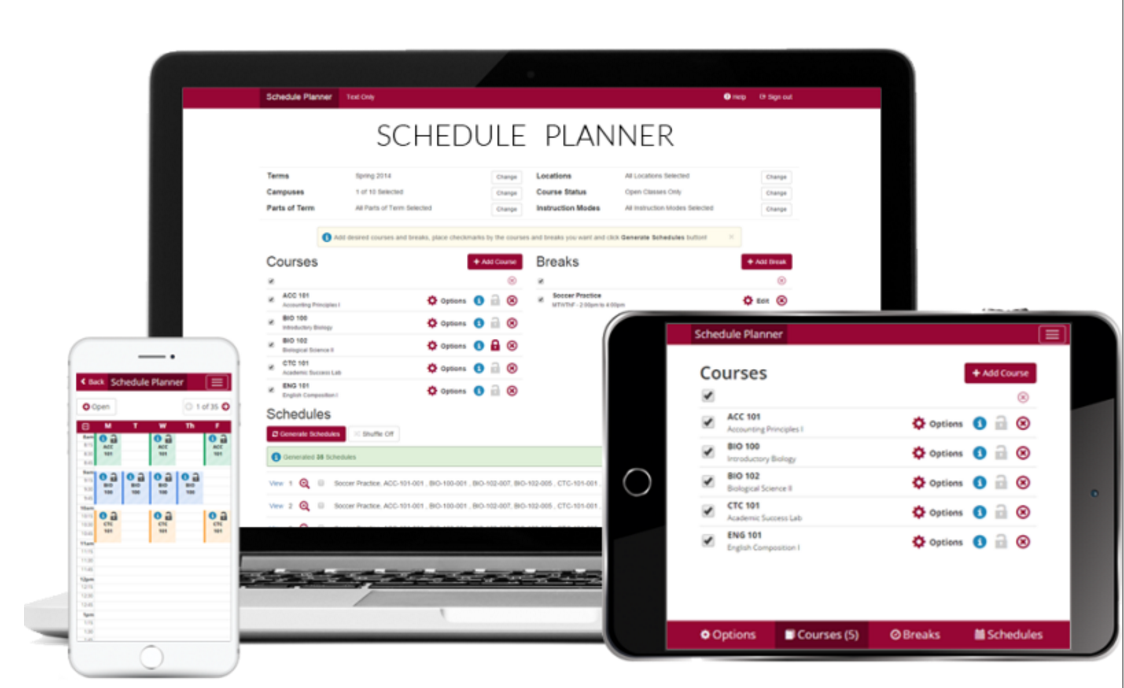
\includegraphics[width=1.0\textwidth]{college_sched_sp}
\caption{Example of Schedule Planner. \textit{Source: http://www.collegescheduler.com/schedule-planner/}}
\end{figure}


\subsubsection{Schedule Planner}
Schedule Planner allows students to easily schedule (or automatically generate) their classes around outside obligations. It also helps students to maximize their credit hours and graduate on time. Schedule Planner also analyzes student preference data to predict the optimal number of course sections to offer and helps to evenly distribute class fill rates. It enables advisers to create course schedules for groups of students at a time. One of their main goals is to allow students to focus on which courses to take rather than worrying about when they are being offered.

\begin{figure}[h]
\centering
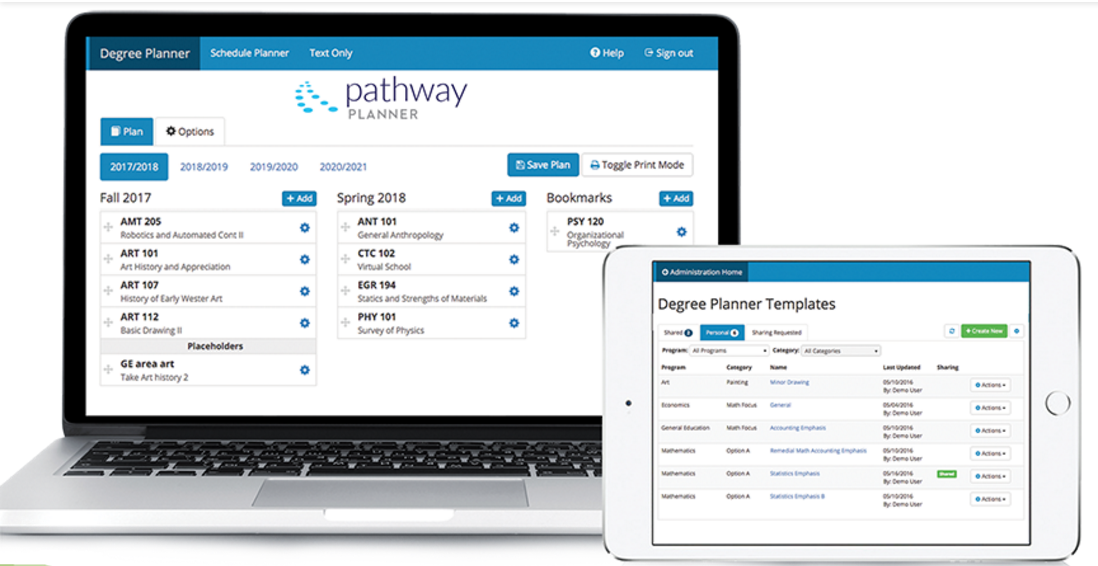
\includegraphics[width=1.0\textwidth]{college_sched_pp}
\caption{Example of Pathway Planner. \textit{Source: http://www.collegescheduler.com/pathway-planner/}}
\end{figure}

\subsubsection{Pathway Planner}
The Pathway Planner allows students to plan their schedules in a multi-year format to encourage seeing the bigger picture and to plan ahead. It provides visuals to show students how their predicted course loads will affect their graduation date. Administrators can also see the courses that students plan on taking before registration. This allows for the addition and elimination of courses to best fit student needs. 

\subsubsection{College Scheduler and Academic/Professional/Social Engagement}
College Scheduler focuses on the scheduling aspect of degree planning. However, it views scheduling as a long term event, and allows students and administrators to work together to offer courses in an optimal manner. While College Scheduler addresses the needs to students as a whole, it does not offer individualized support based off individual needs. Every student has different goals, plans, and schedules, and there is no one master schedule that can accommodate them all. However, if it were to offer individual support on a case by case basis, it would be able to help a larger amount of students to reach their unique goals. 

\begin{figure}[h]
\centering
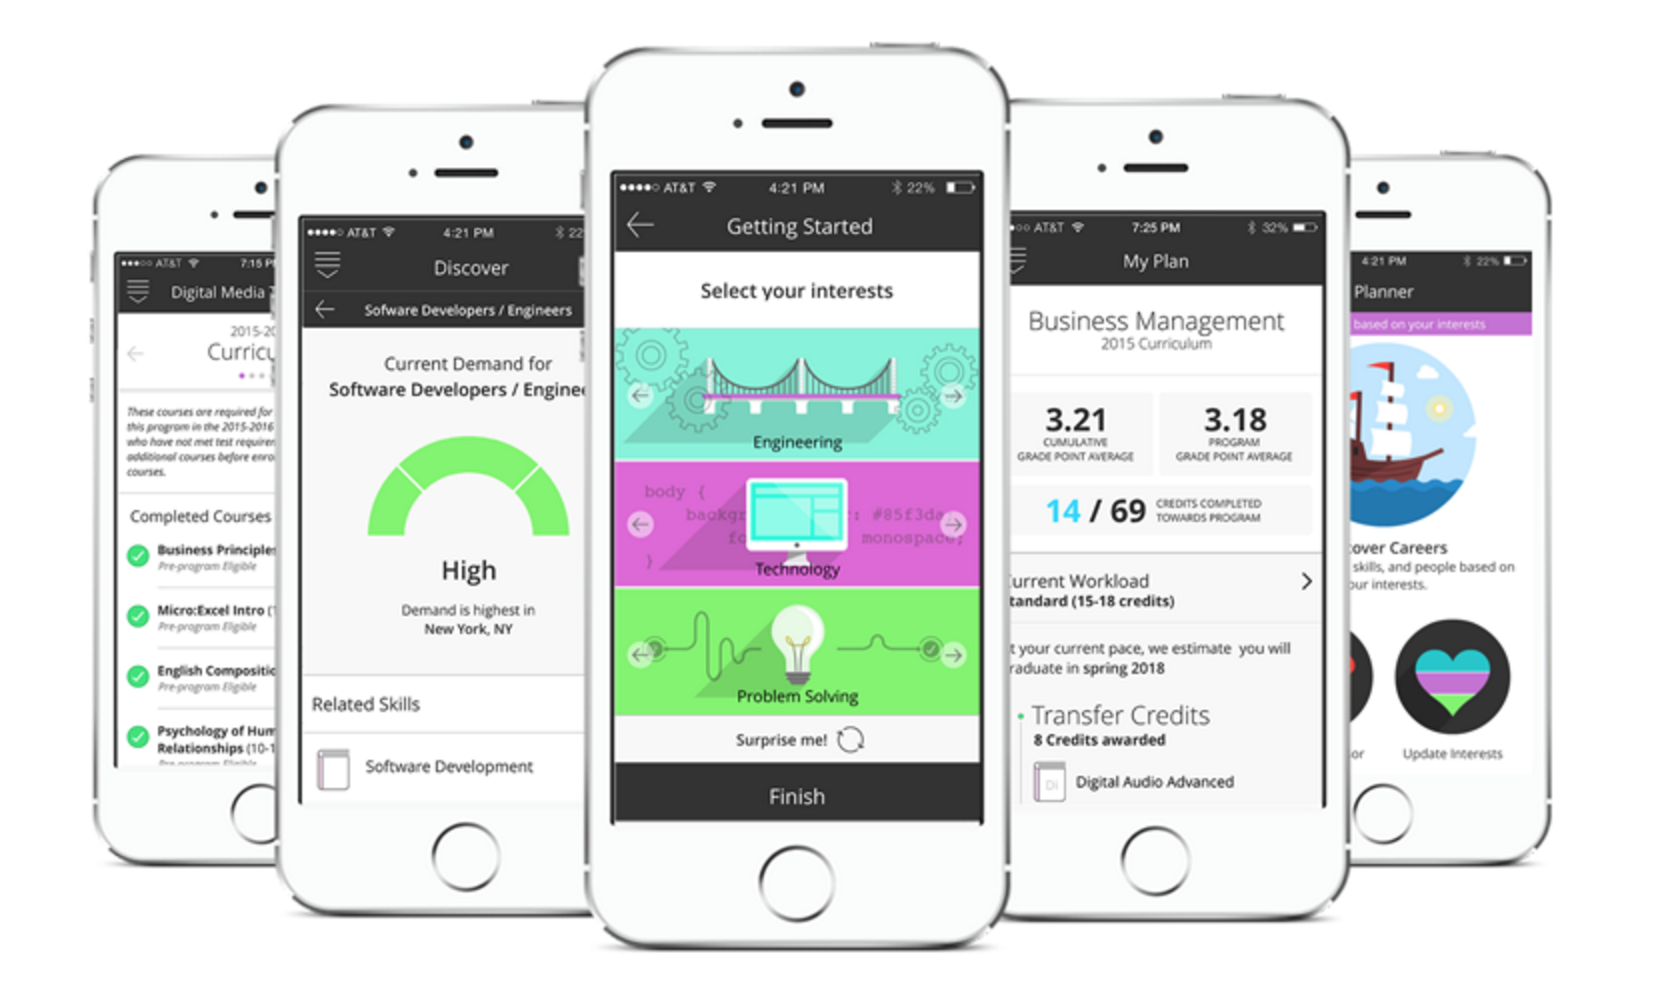
\includegraphics[width=1.0\textwidth]{blackboard_students}
\caption{Example student view of the Blackboard Planner mobile application screens. \textit{Source: http://www.blackboard.com/mobile-learning/planner.aspx}}
\end{figure}
\subsection{Blackboard Planner} 
Blackboard recently bought out the college planning system MyEdu to create a new mobile student planning application called Blackboard Planner. The main goals of Blackboard Planner are to improve student outcomes, simplify planning, and provide better support. Since the system was released in October 2016, at the time of writing, there currently is not much information regarding the system and it's usage.

\subsubsection{Improve Student Outcomes}
Blackboard Planner aims to improve student outcomes by providing students with real labor demand information from Burning Glass and Roadtrip Nation, which can ideally allow students to make better academic and career decisions.

\subsubsection{Simplify Planning}
Blackboard Planner aims to simplify planning by offering customized scheduling, hassle-free registration, and an academic plan tracker. These features are aimed at helping students graduate on time.

\begin{figure}[h]
\centering
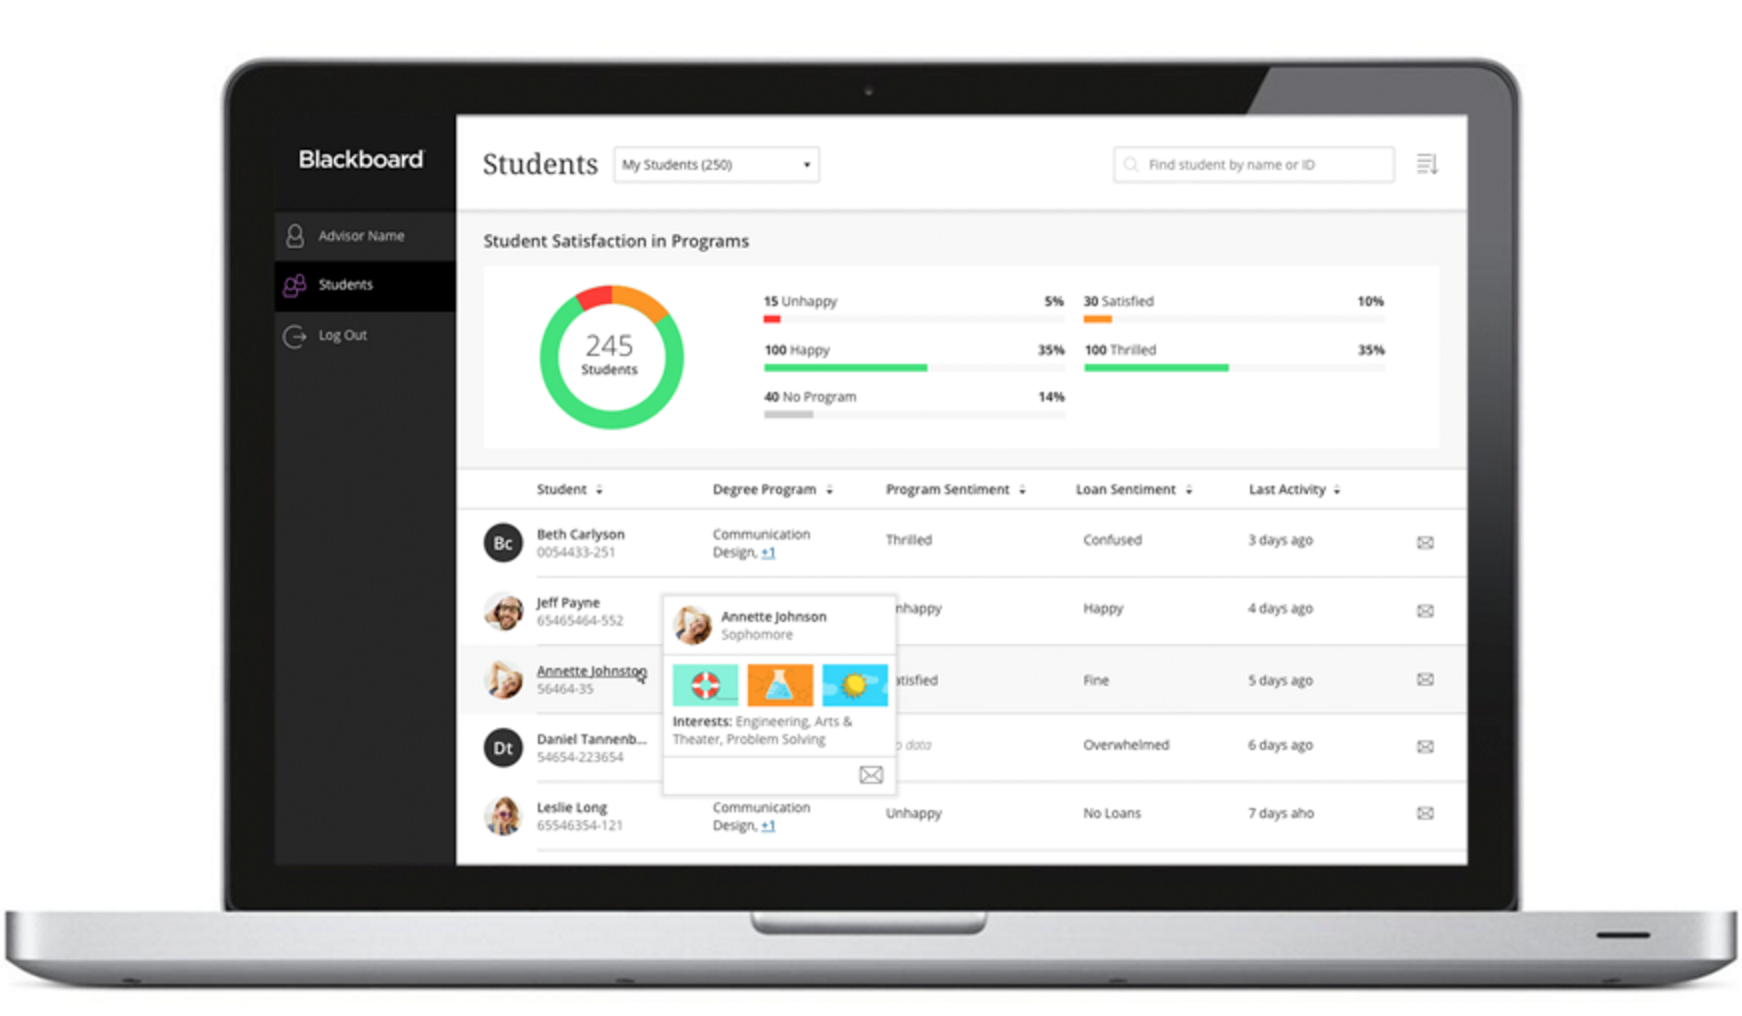
\includegraphics[width=1.0\textwidth]{blackboard_adviser}
\caption{Example adviser view of Blackboard Planner. \textit{Source: http://www.blackboard.com/mobile-learning/planner.aspx}}
\end{figure}

\subsubsection{Provide Better Support}
Blackboard Planner provides an adviser view which allows advisers to combine their insight into the student's academic plans, student sentiment, and predictive analysis together to offer well-informed support to students. 

\subsubsection{Blackboard Planner and Academic/Professional/Social Engagement}
With the limited information available about Blackboard Planner, it seems to address many degree planning problems that older degree planners, such as STAR, Starfish by Hobsons, and College Scheduler do not. For instance, Blackboard Planner uses job market analytic services to provide students with the most relevant and up to date information regarding careers. However, while Blackboard Planner seems to excel at offering post-graduation advice, it seems to be lacking in pre-graduation advice. Blackboard Planner does not offer course advice to fit the student's current lifestyle, taking work and extracurricular activities into consideration. Planning for the future is important, but students must remember to plan for the present as well. 

\begin{figure}[h]
\centering
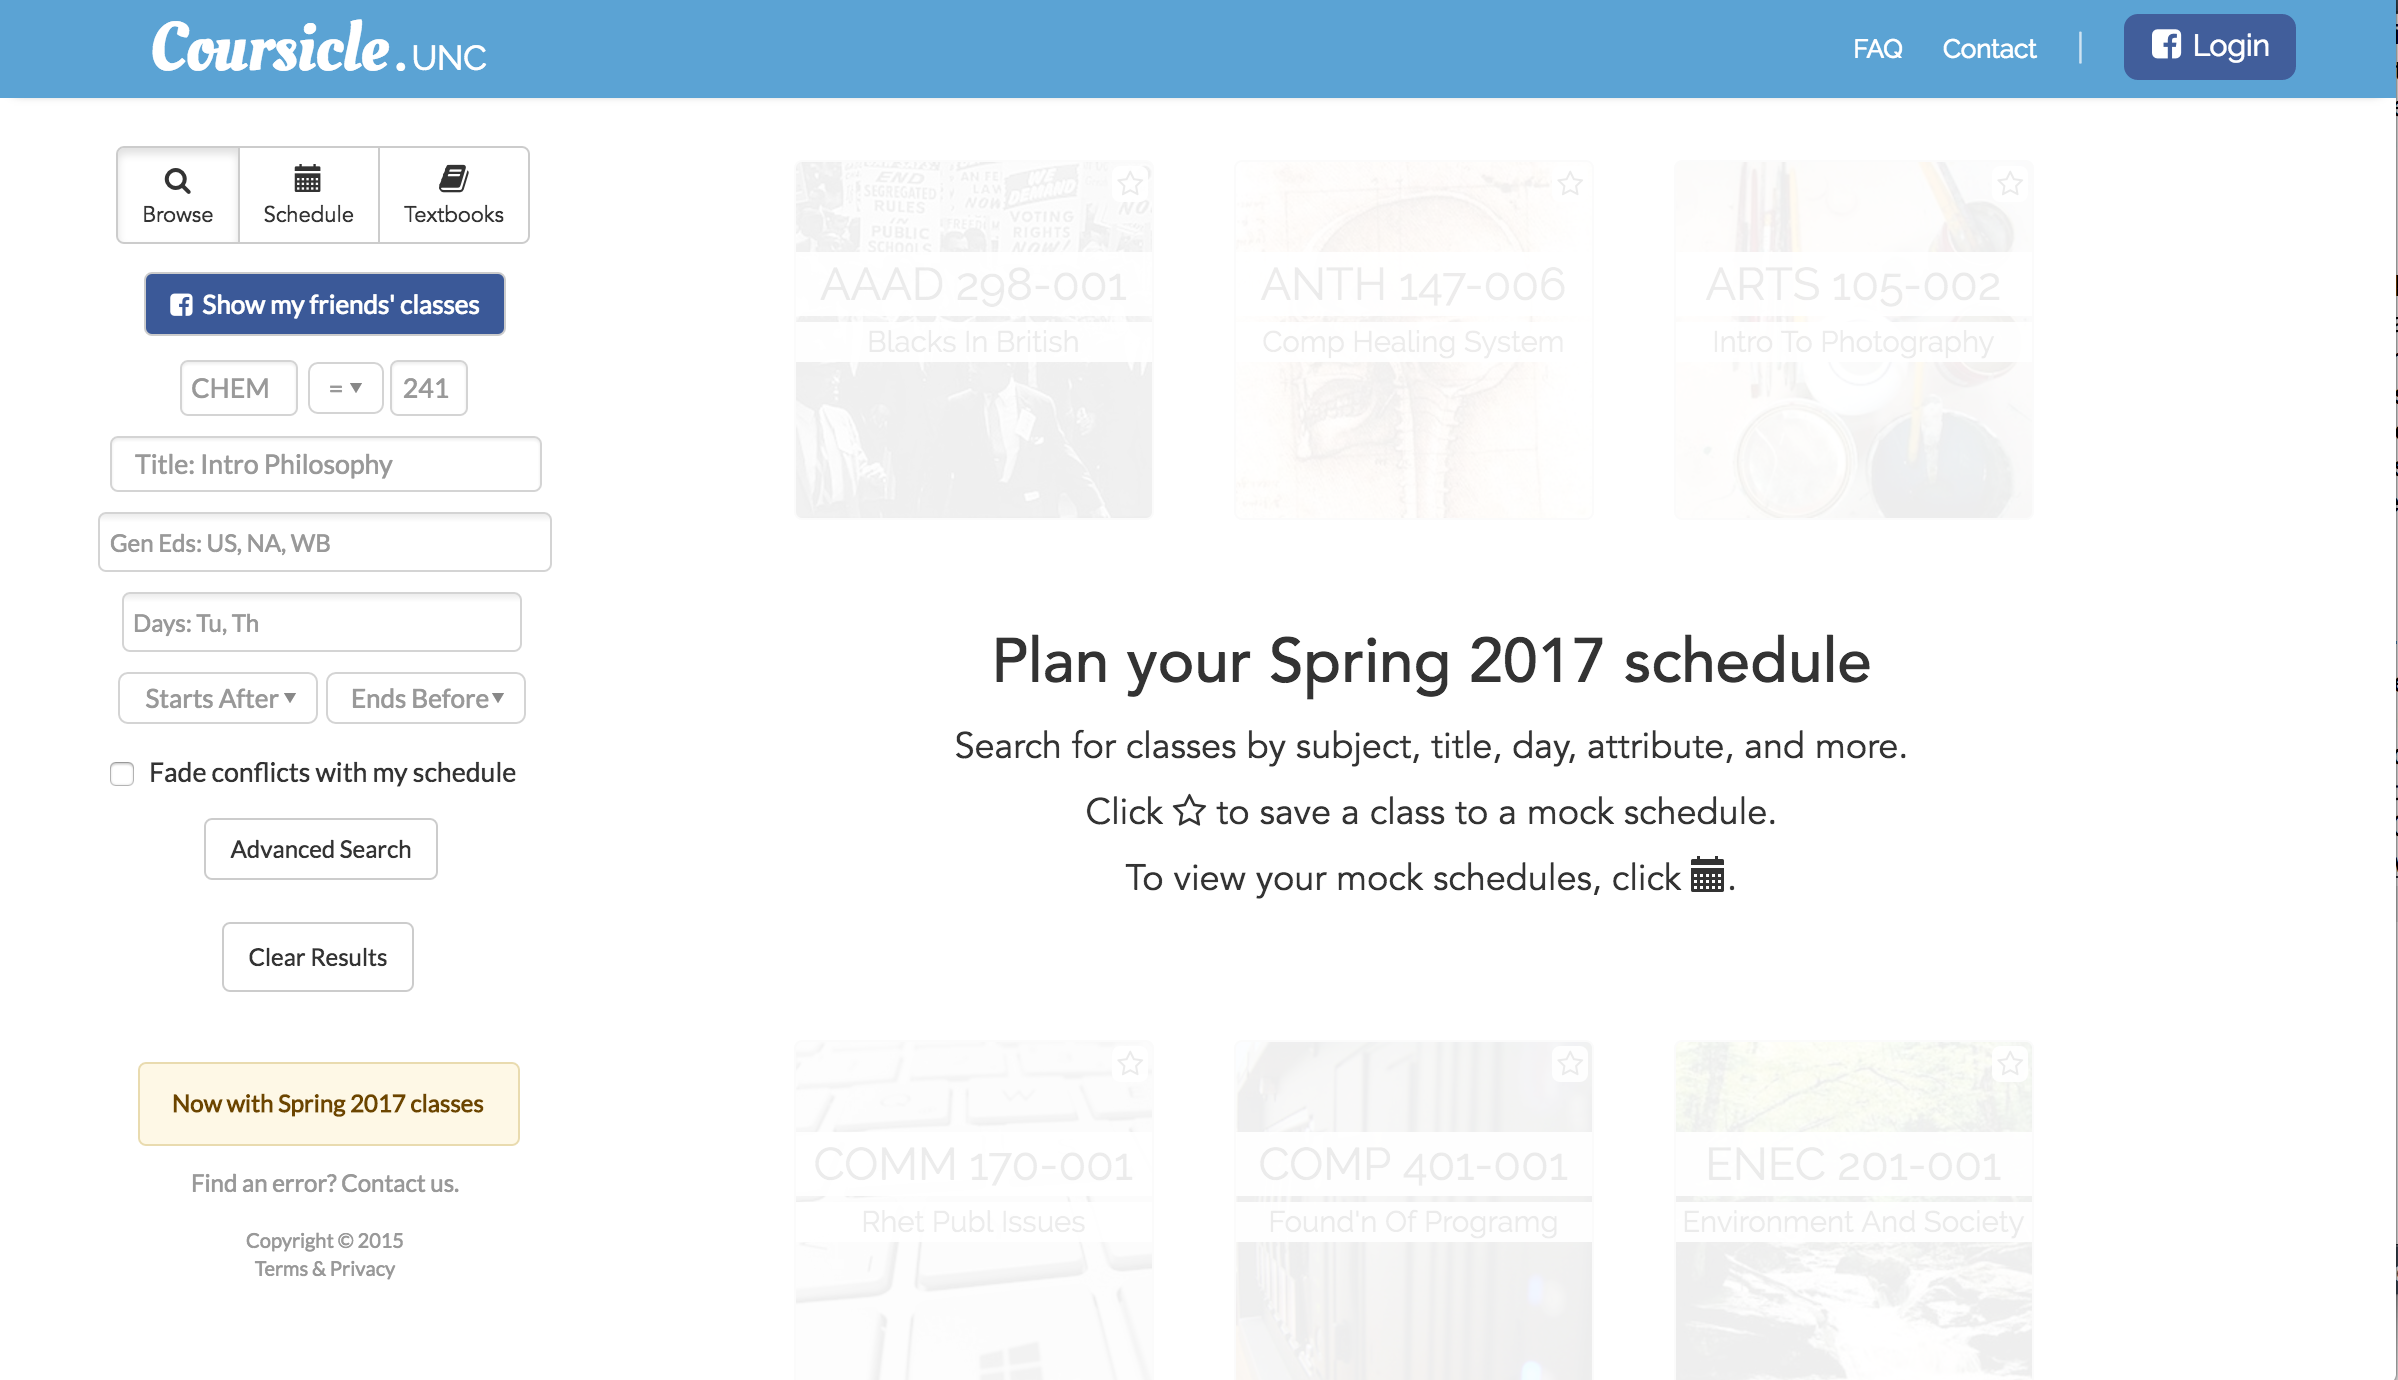
\includegraphics[width=1.0\textwidth]{coursicle}
\caption{The Coursicle page for the University of North Carolina.\textit{Source: https://www.coursicle.com/unc/}}
\end{figure}
\subsection{Coursicle}
The slogan of Coursicle is ``Course registration sucks but Coursicle makes it better." The features of Coursicle are: students can receive text or email notifications when a seat opens up in class, students can schedule their courses using an attractive schedule planner, students can search through courses more easily with a variety of filters, students can create schedules with all prospective classes and then narrow them down to one workable schedule, students can easily compare textbook prices online through Coursicle, and students can view what classes their classmates are signed up for via Facebook. 

\subsubsection{Coursicle and Academic/Professional/Social Engagement}
Coursicle is focused on making students happy by making registration easier and more enjoyable. However, although Coursicle makes it easier, it does not suggest classes to students based off their goals and previous coursework. Coursicle definitely helps alleviate the psychological pain of registration, but it does not alleviate the overall ongoing pain of degree planning. 

\subsection{Individual Student Software and Academic/Professional/Social Engagement}
There are other types of download-able software currently available for students to use individually. These systems are for individual use, and are not tailored for institutional implementation. To use these systems, students input information about their education, such as classes, credits, and requirements. This data is then used to create organized visualizations to help students to better see their goals and pathway. A popular generic system is the Microsoft Office College Credit Planner Template. Many individual colleges and universities have their own custom download-able course planning spreadsheets as well. While these systems help students to organize the data they have, they do not offer any new ideas or suggestions for further improvement.

\section{Social Network}
\subsection{LinkedIn}
LinkedIn is widely known for being the world's largest professional network. It sets itself apart from other popular social media sites by being focused solely on building professional identities and forging professional relationships. There are six major components to LinkedIn: Home, Profile, My Network, Learning, Jobs, and Interests.

\begin{figure}[h]
\centering
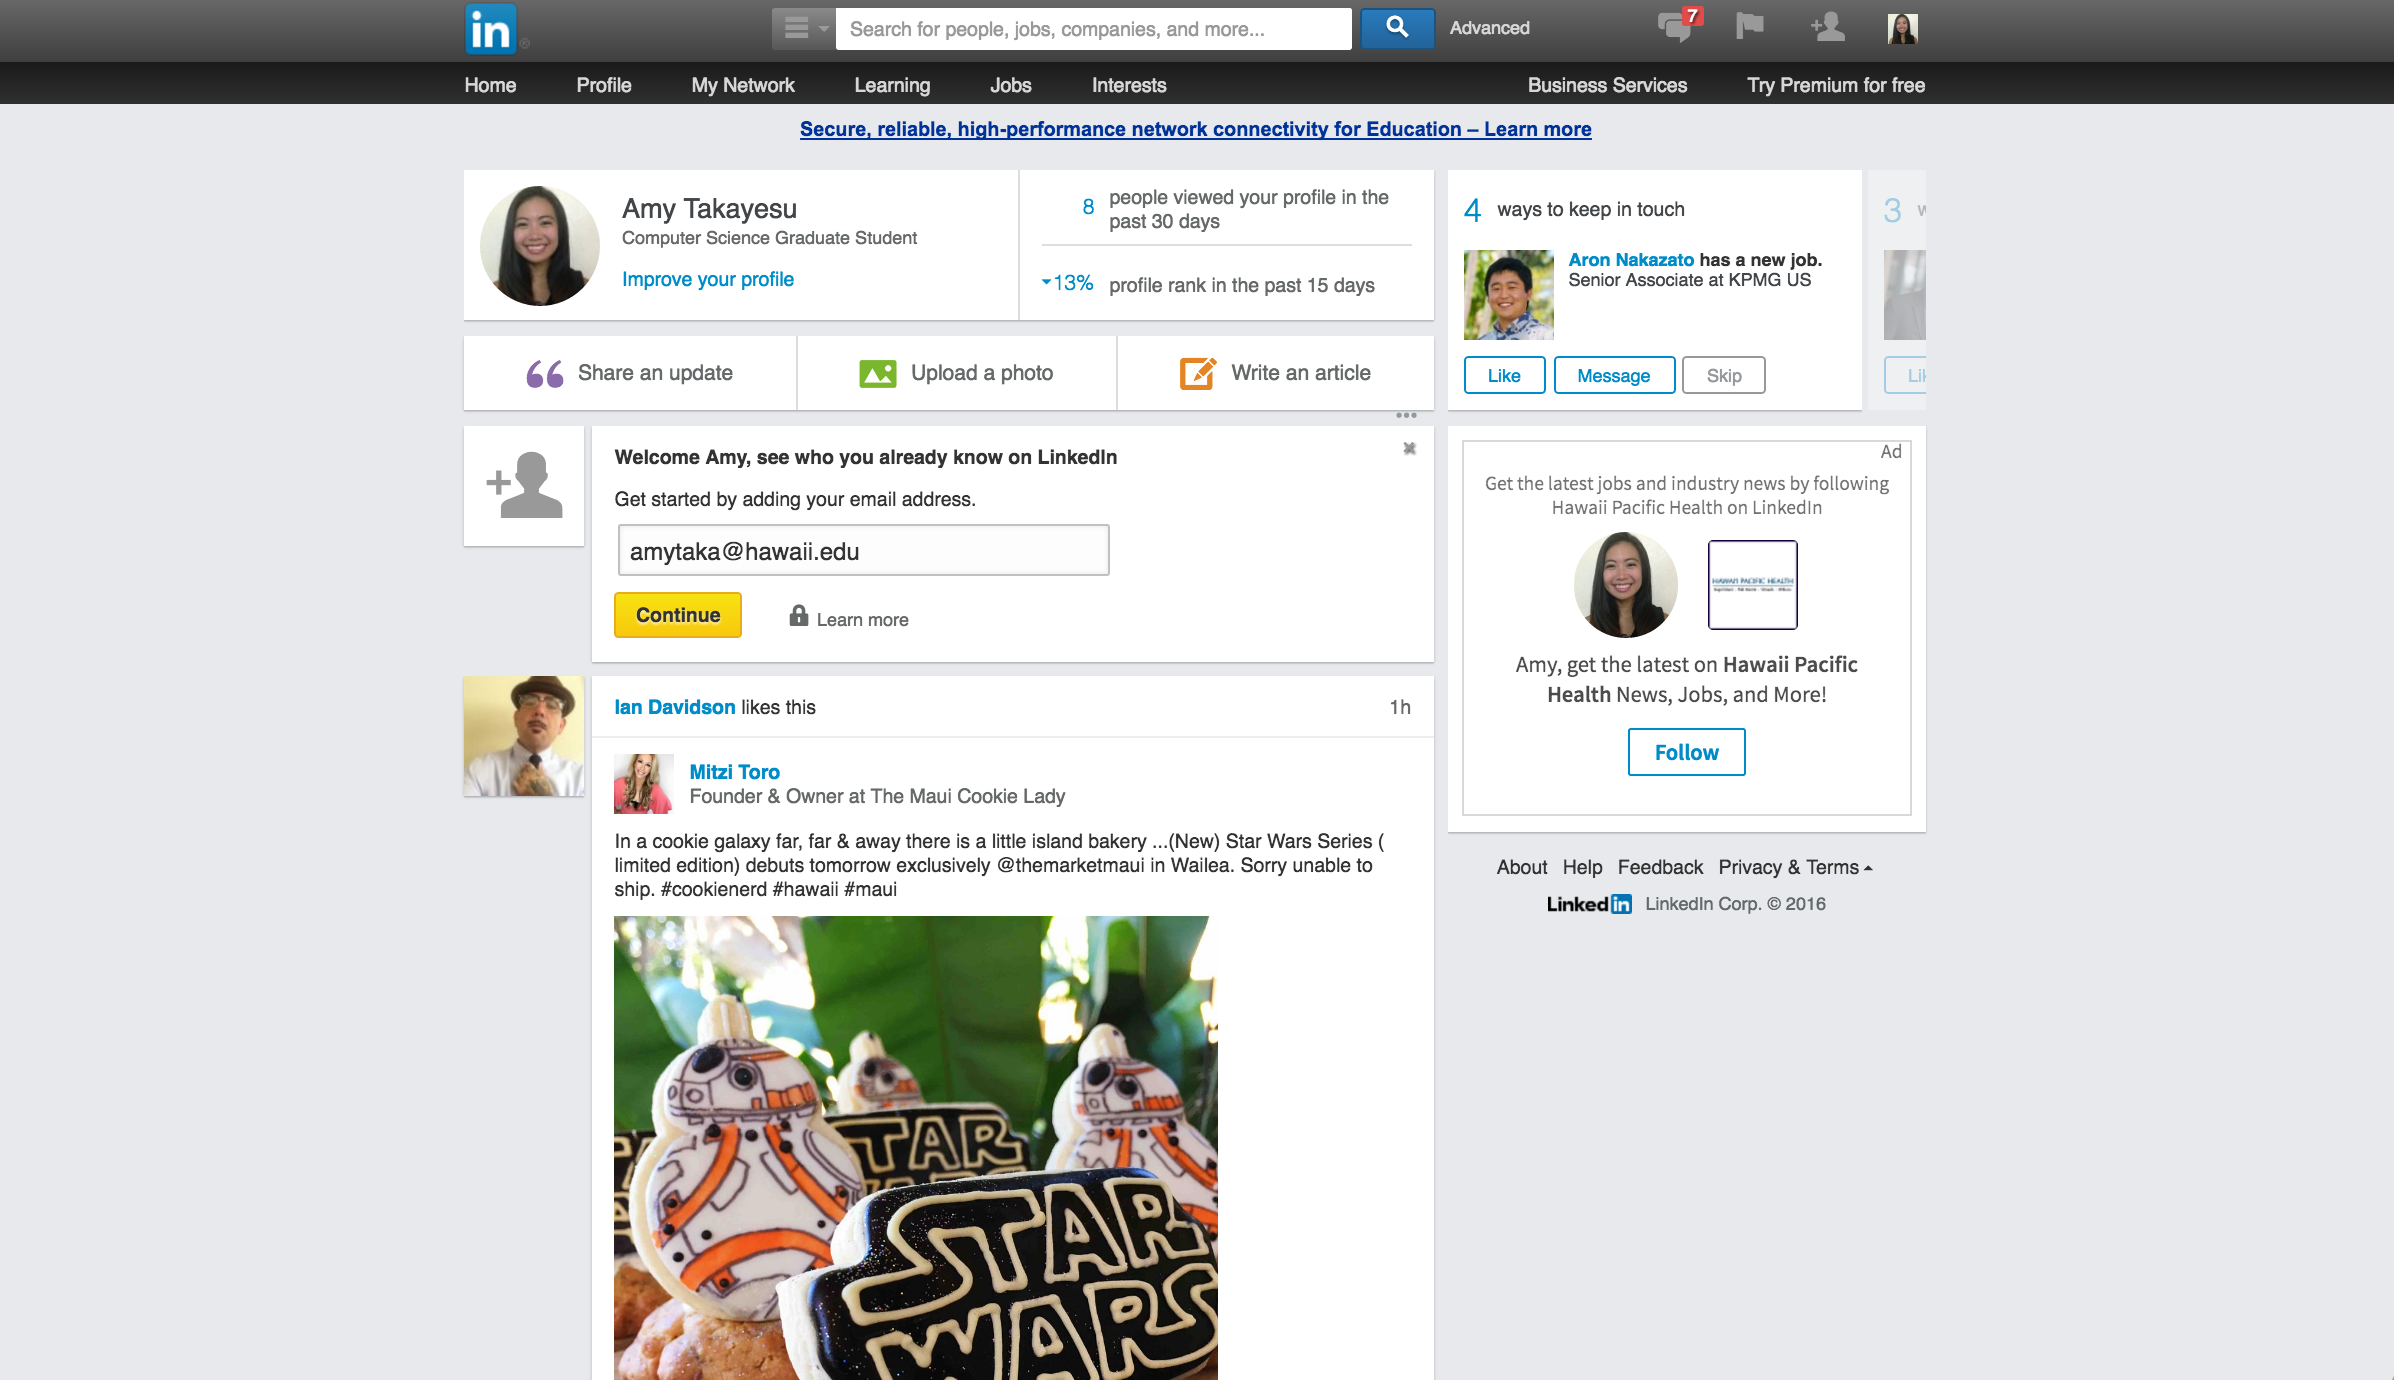
\includegraphics[width=1.0\textwidth]{linkedin_home}
\caption{LinkedIn homepage. \textit{Source: http://www.linkedin.com}}
\end{figure}

\subsubsection{Home}
A user's homepage is arranged in a feed type format, with quick information about your profile, profile views, and incoming messages. The feed section contains recent updates from connections and companies related to your interests. There are also sections that encourage engagement--for instance, quick ways to ``share an update", ``upload a photo", or ``write an article" and suggestions to ``reconnect with your colleagues" and to add someone you may know. 

\begin{figure}[h]
\centering
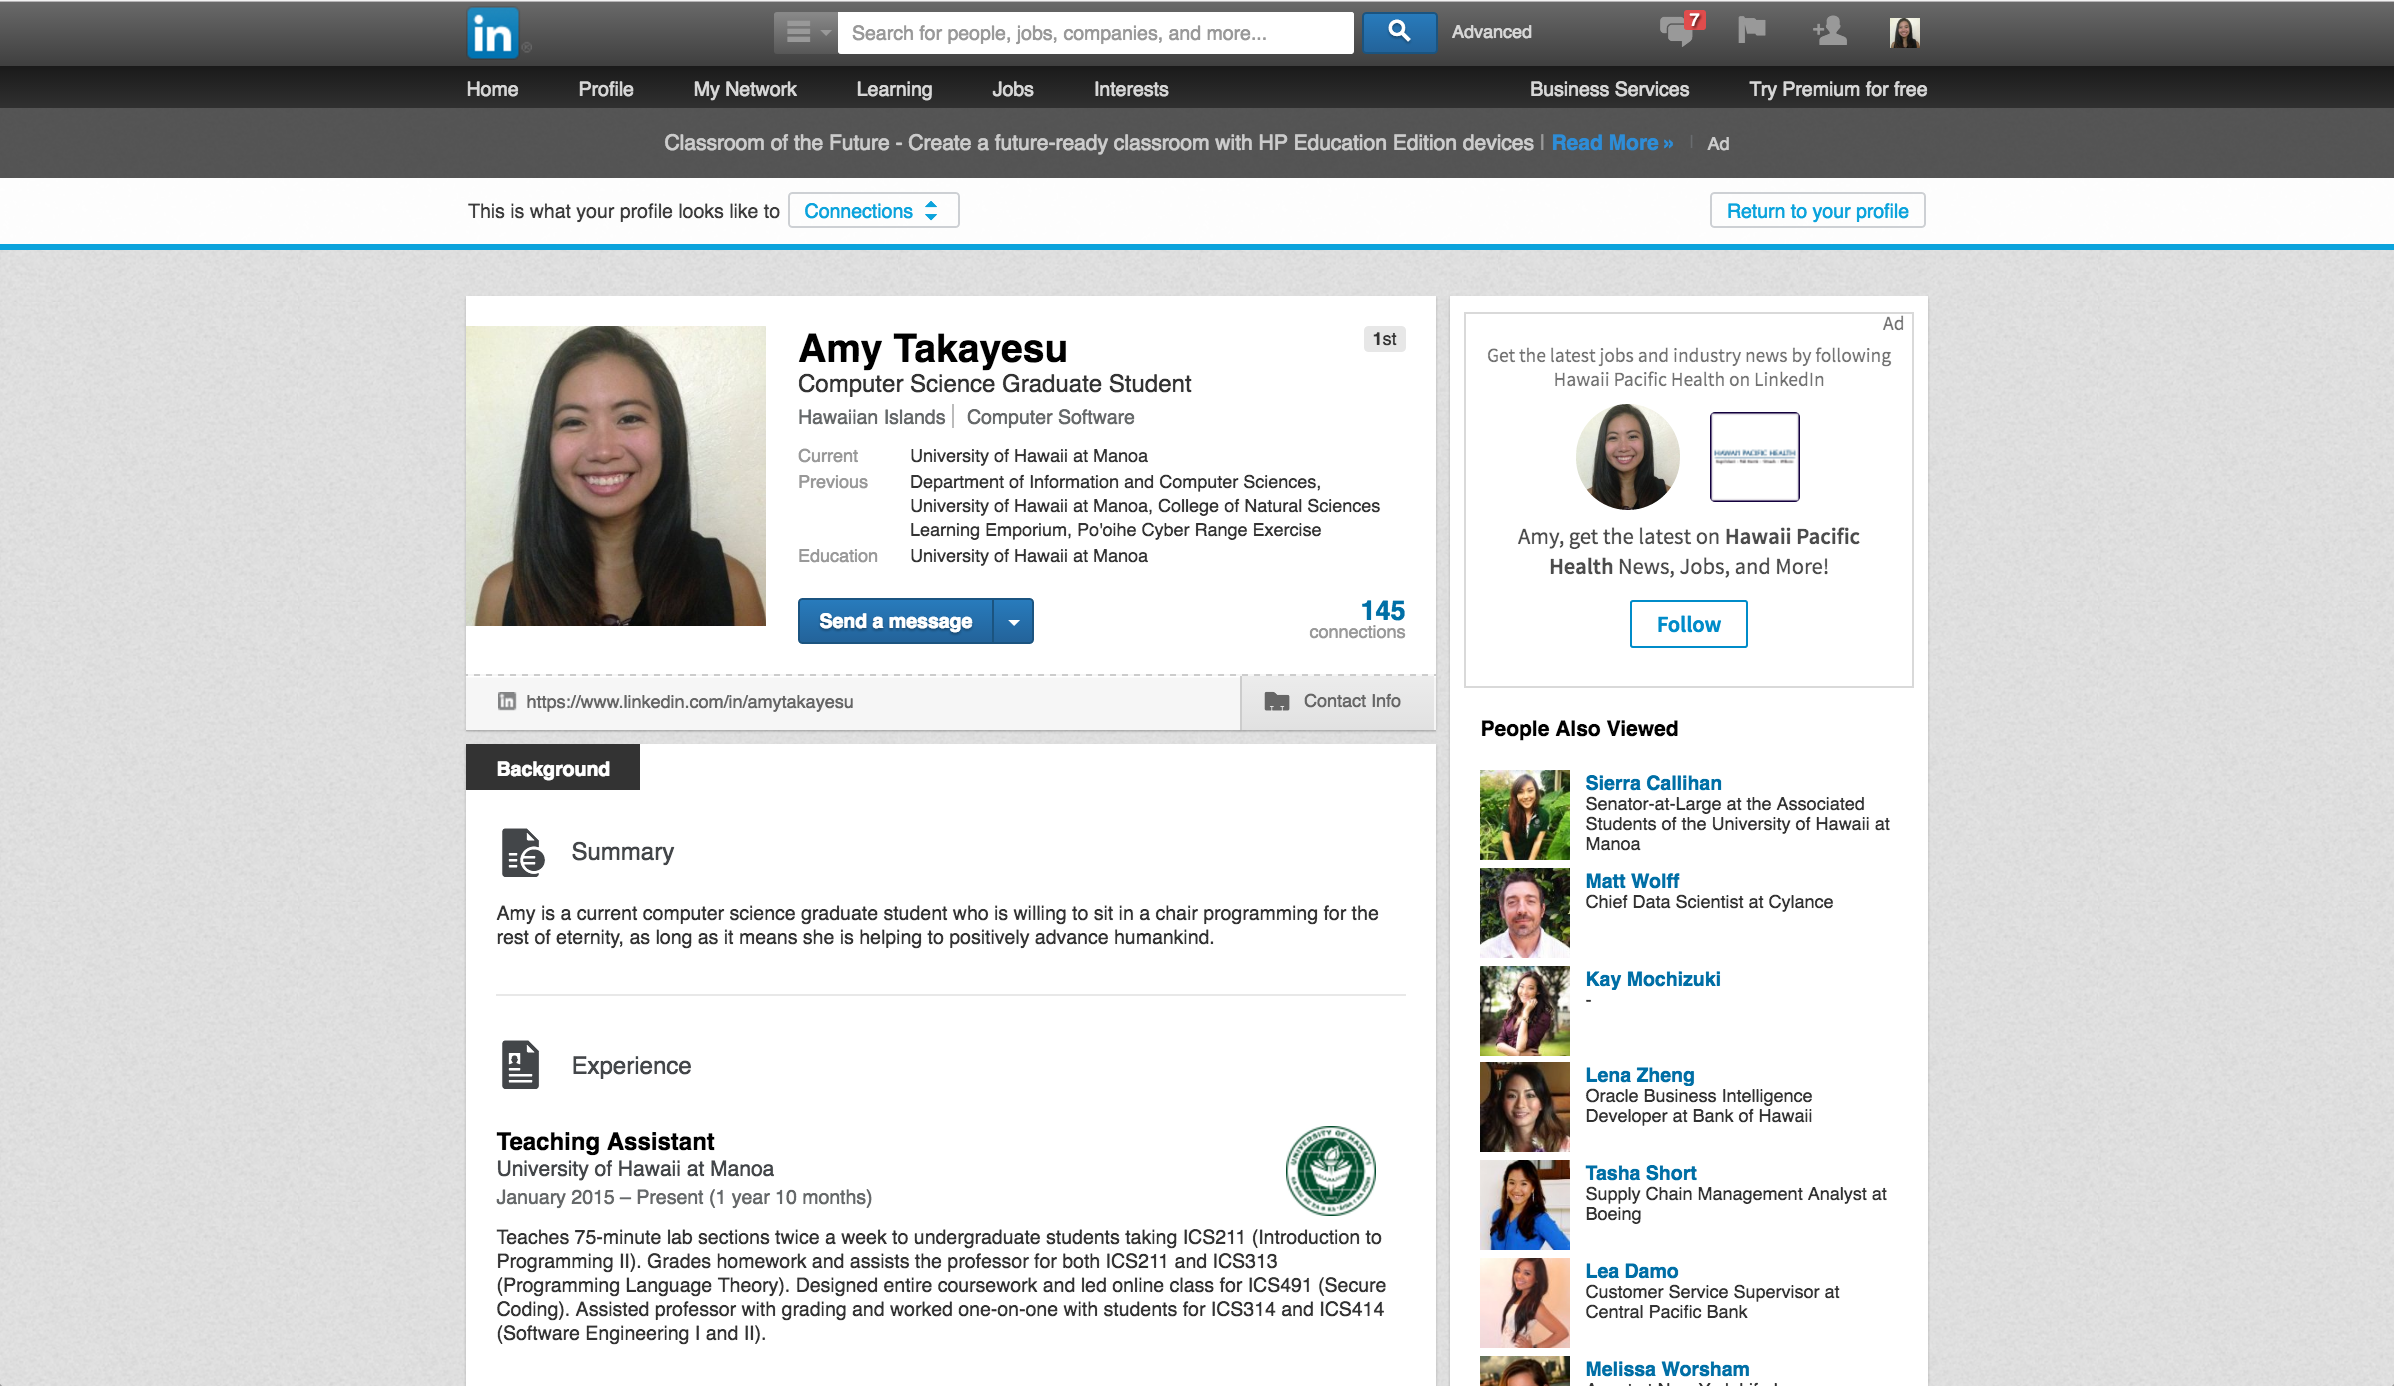
\includegraphics[width=1.0\textwidth]{linkedin_profile}
\caption{LinkedIn profile. \textit{Source: http://www.linkedin.com}}
\end{figure}
\subsubsection{Profile}
A user's profile page is available for other LinkedIn users to see. Users can decide what information they would like to share about themselves, but it is all limited to professional related categories such as education, work experience, volunteer work, and skills and endorsements. 

\begin{figure}[h]
\centering
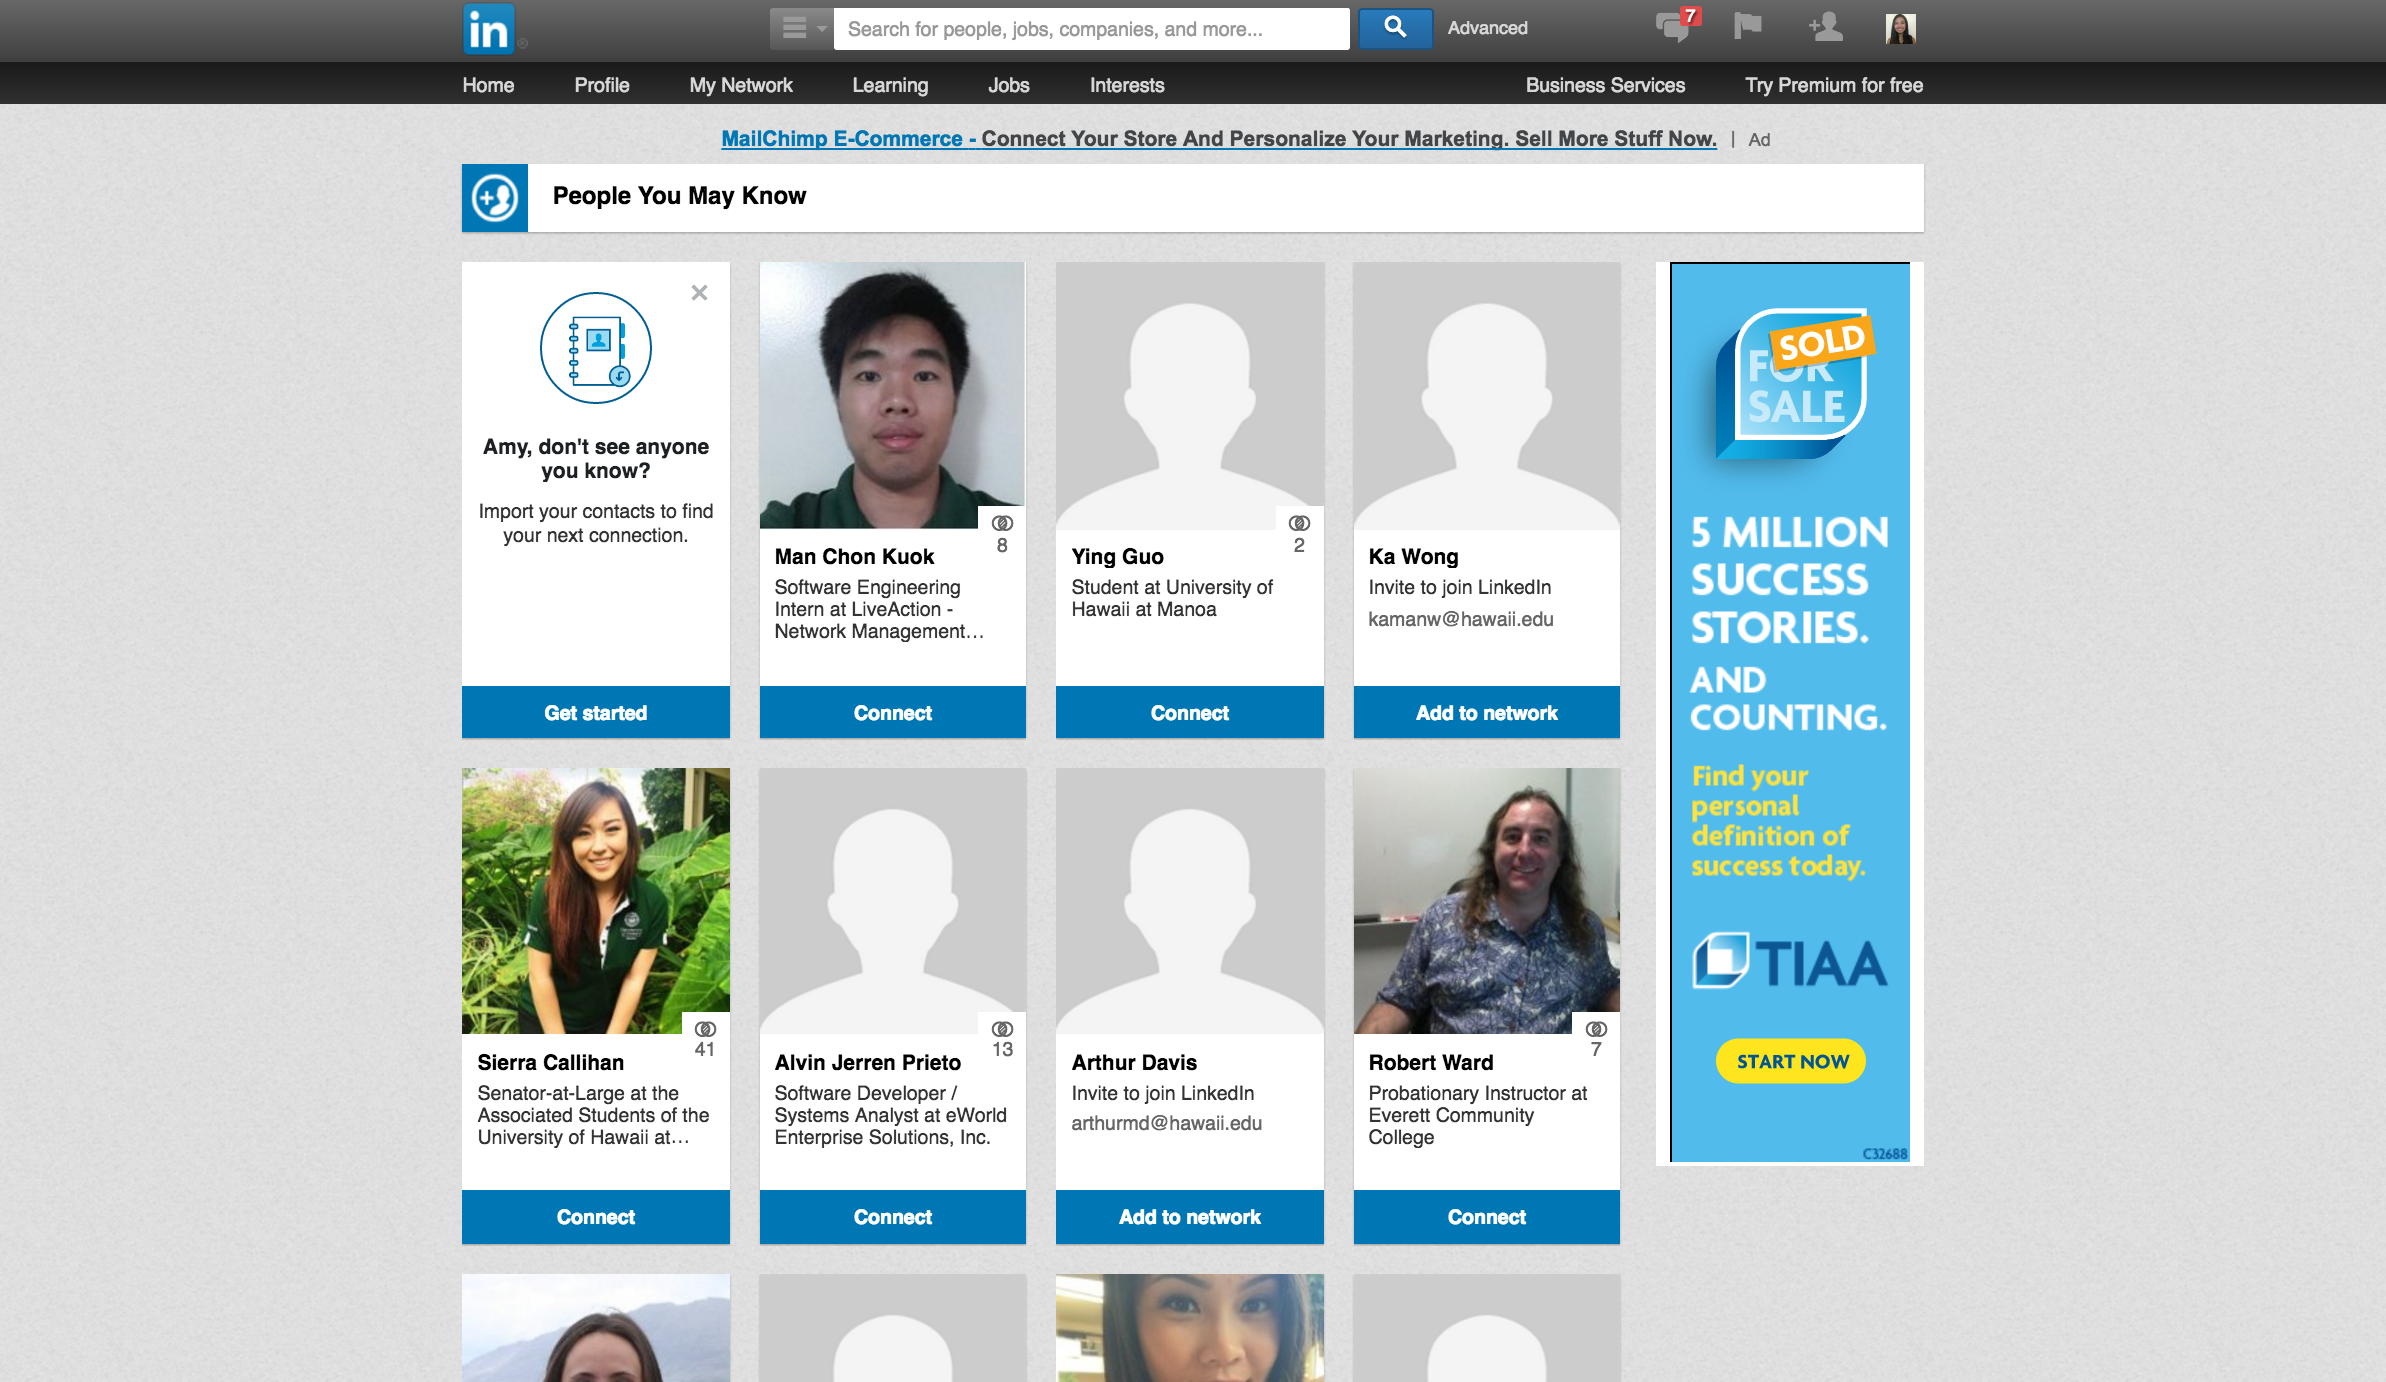
\includegraphics[width=1.0\textwidth]{linkedin_network}
\caption{LinkedIn network page. \textit{Source: http://www.linkedin.com}}
\end{figure}
\subsubsection{My Network}
A user's network includes current connections, recommended connections, connections added through outside contact information, and contacts added through an alumni network. 

\begin{figure}[h]
\centering
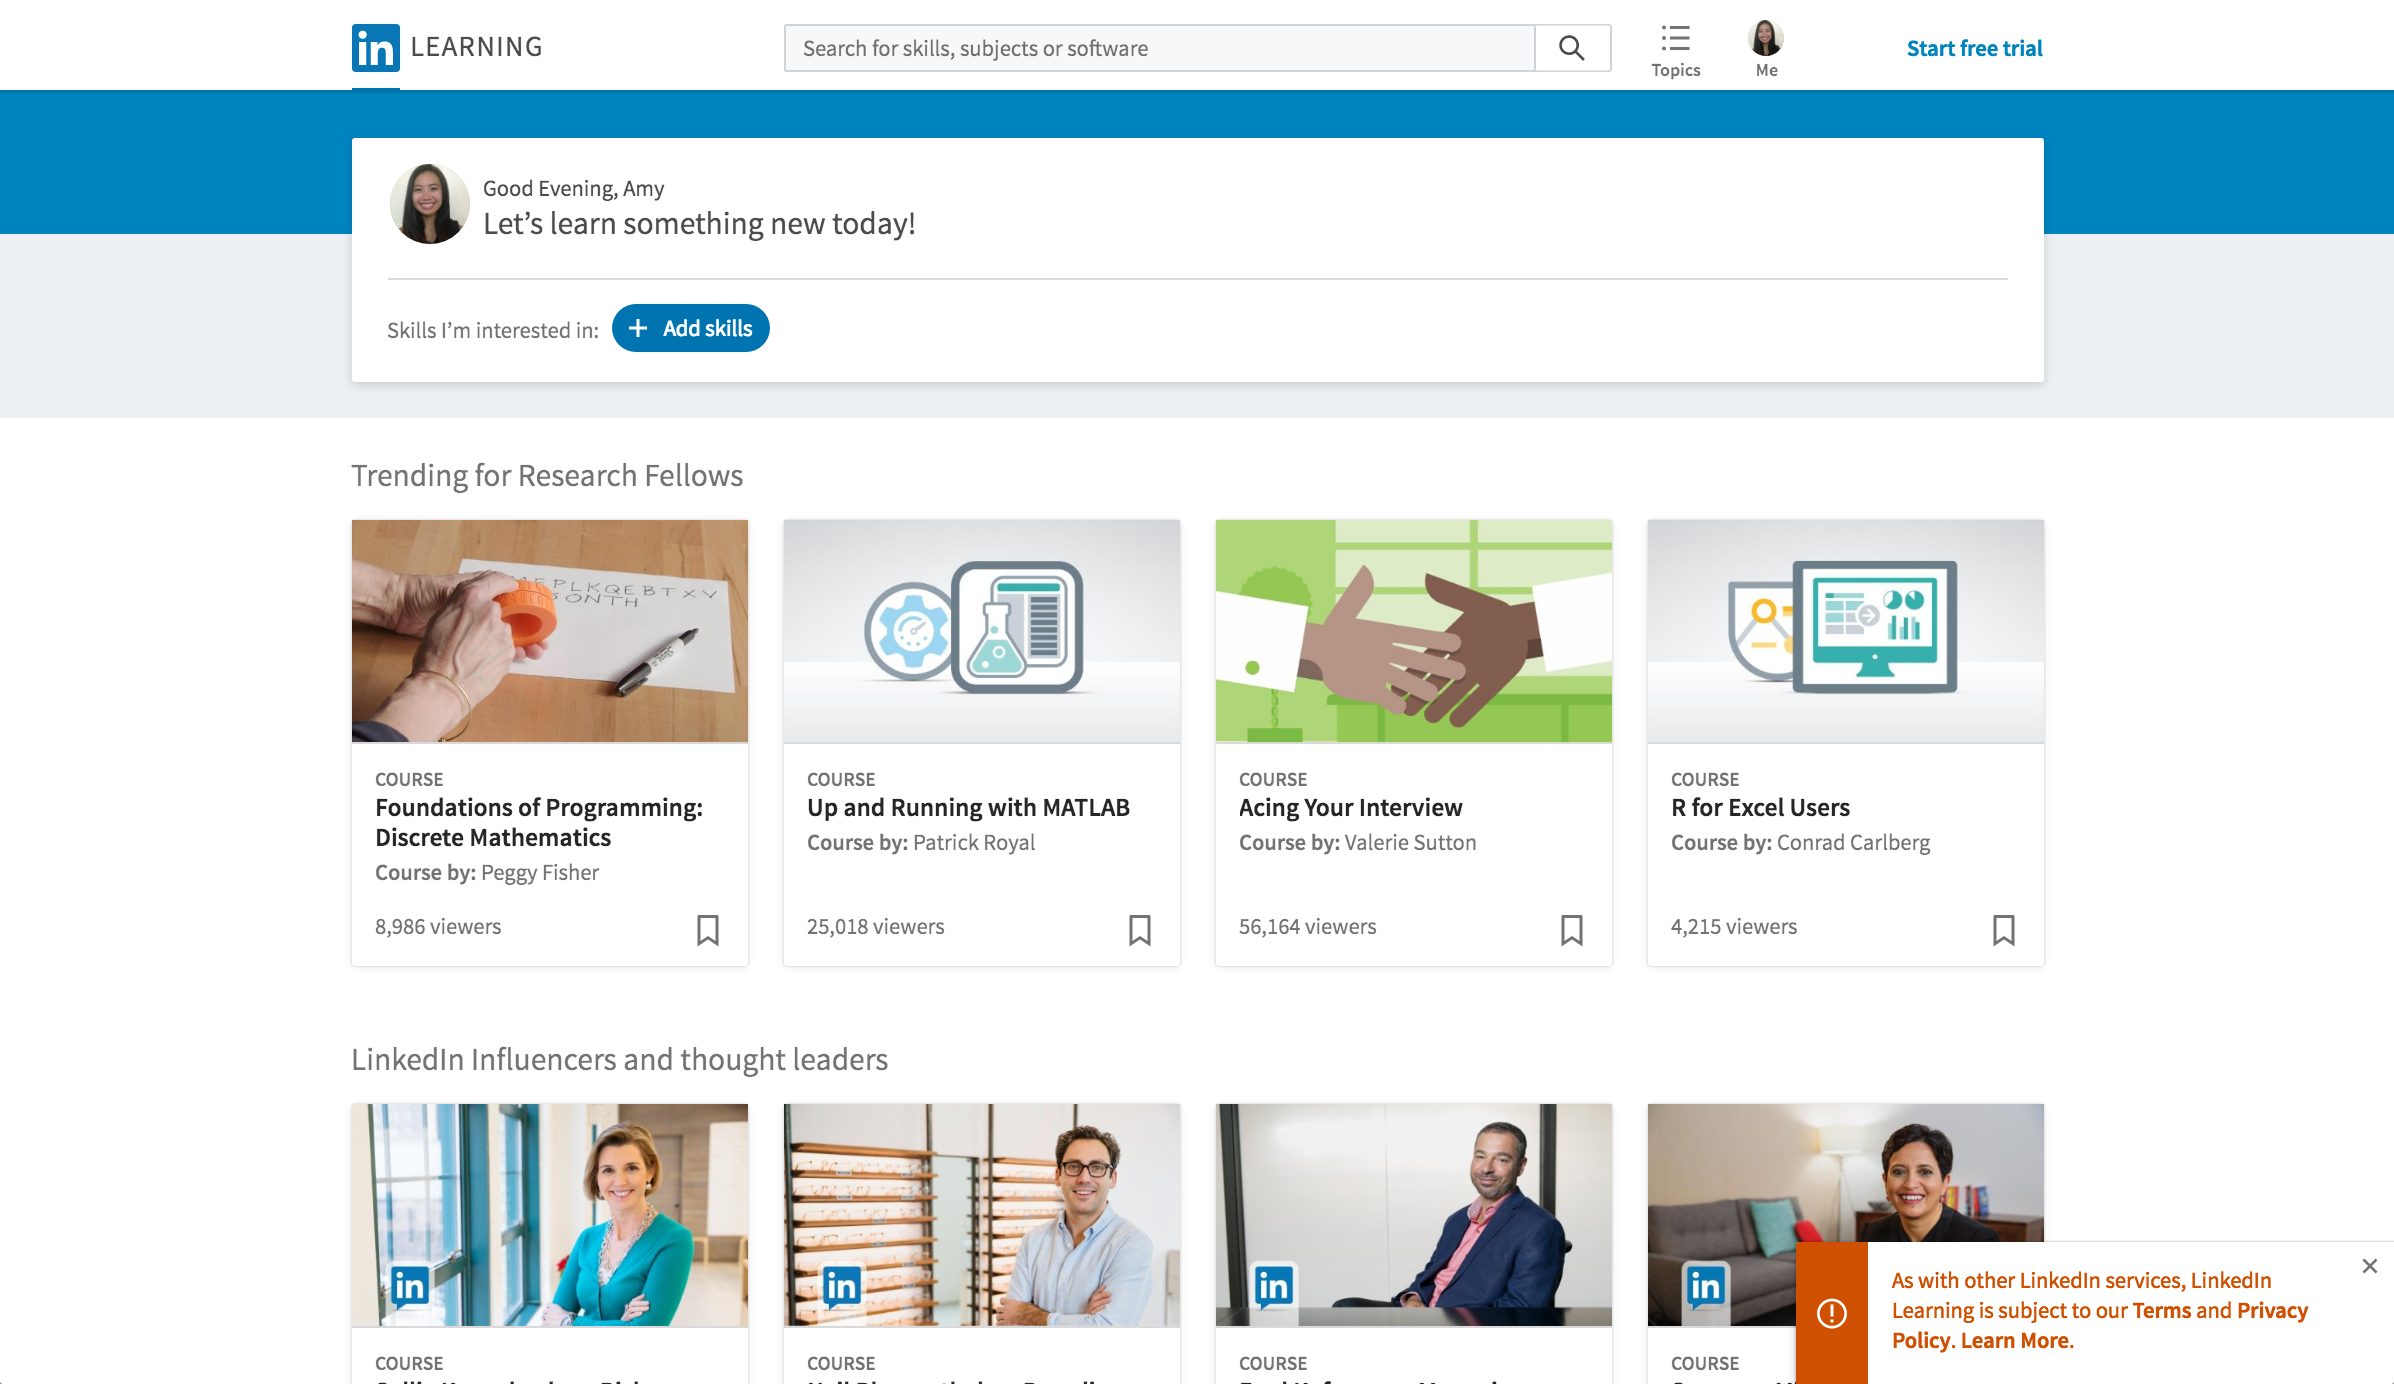
\includegraphics[width=1.0\textwidth]{linkedin_learning}
\caption{LinkedIn learning page. \textit{Source: http://www.linkedin.com}}
\end{figure}
\subsubsection{Learning}
LinkedIn offers online courses on professional development topics such as leadership, storytelling, creating alliances with employees, and winning back a lost customer. There are also field-related courses, such as online code courses. These courses are often in the form of videos, and can be accessed by premium LinkedIn members. 

\begin{figure}[h]
\centering
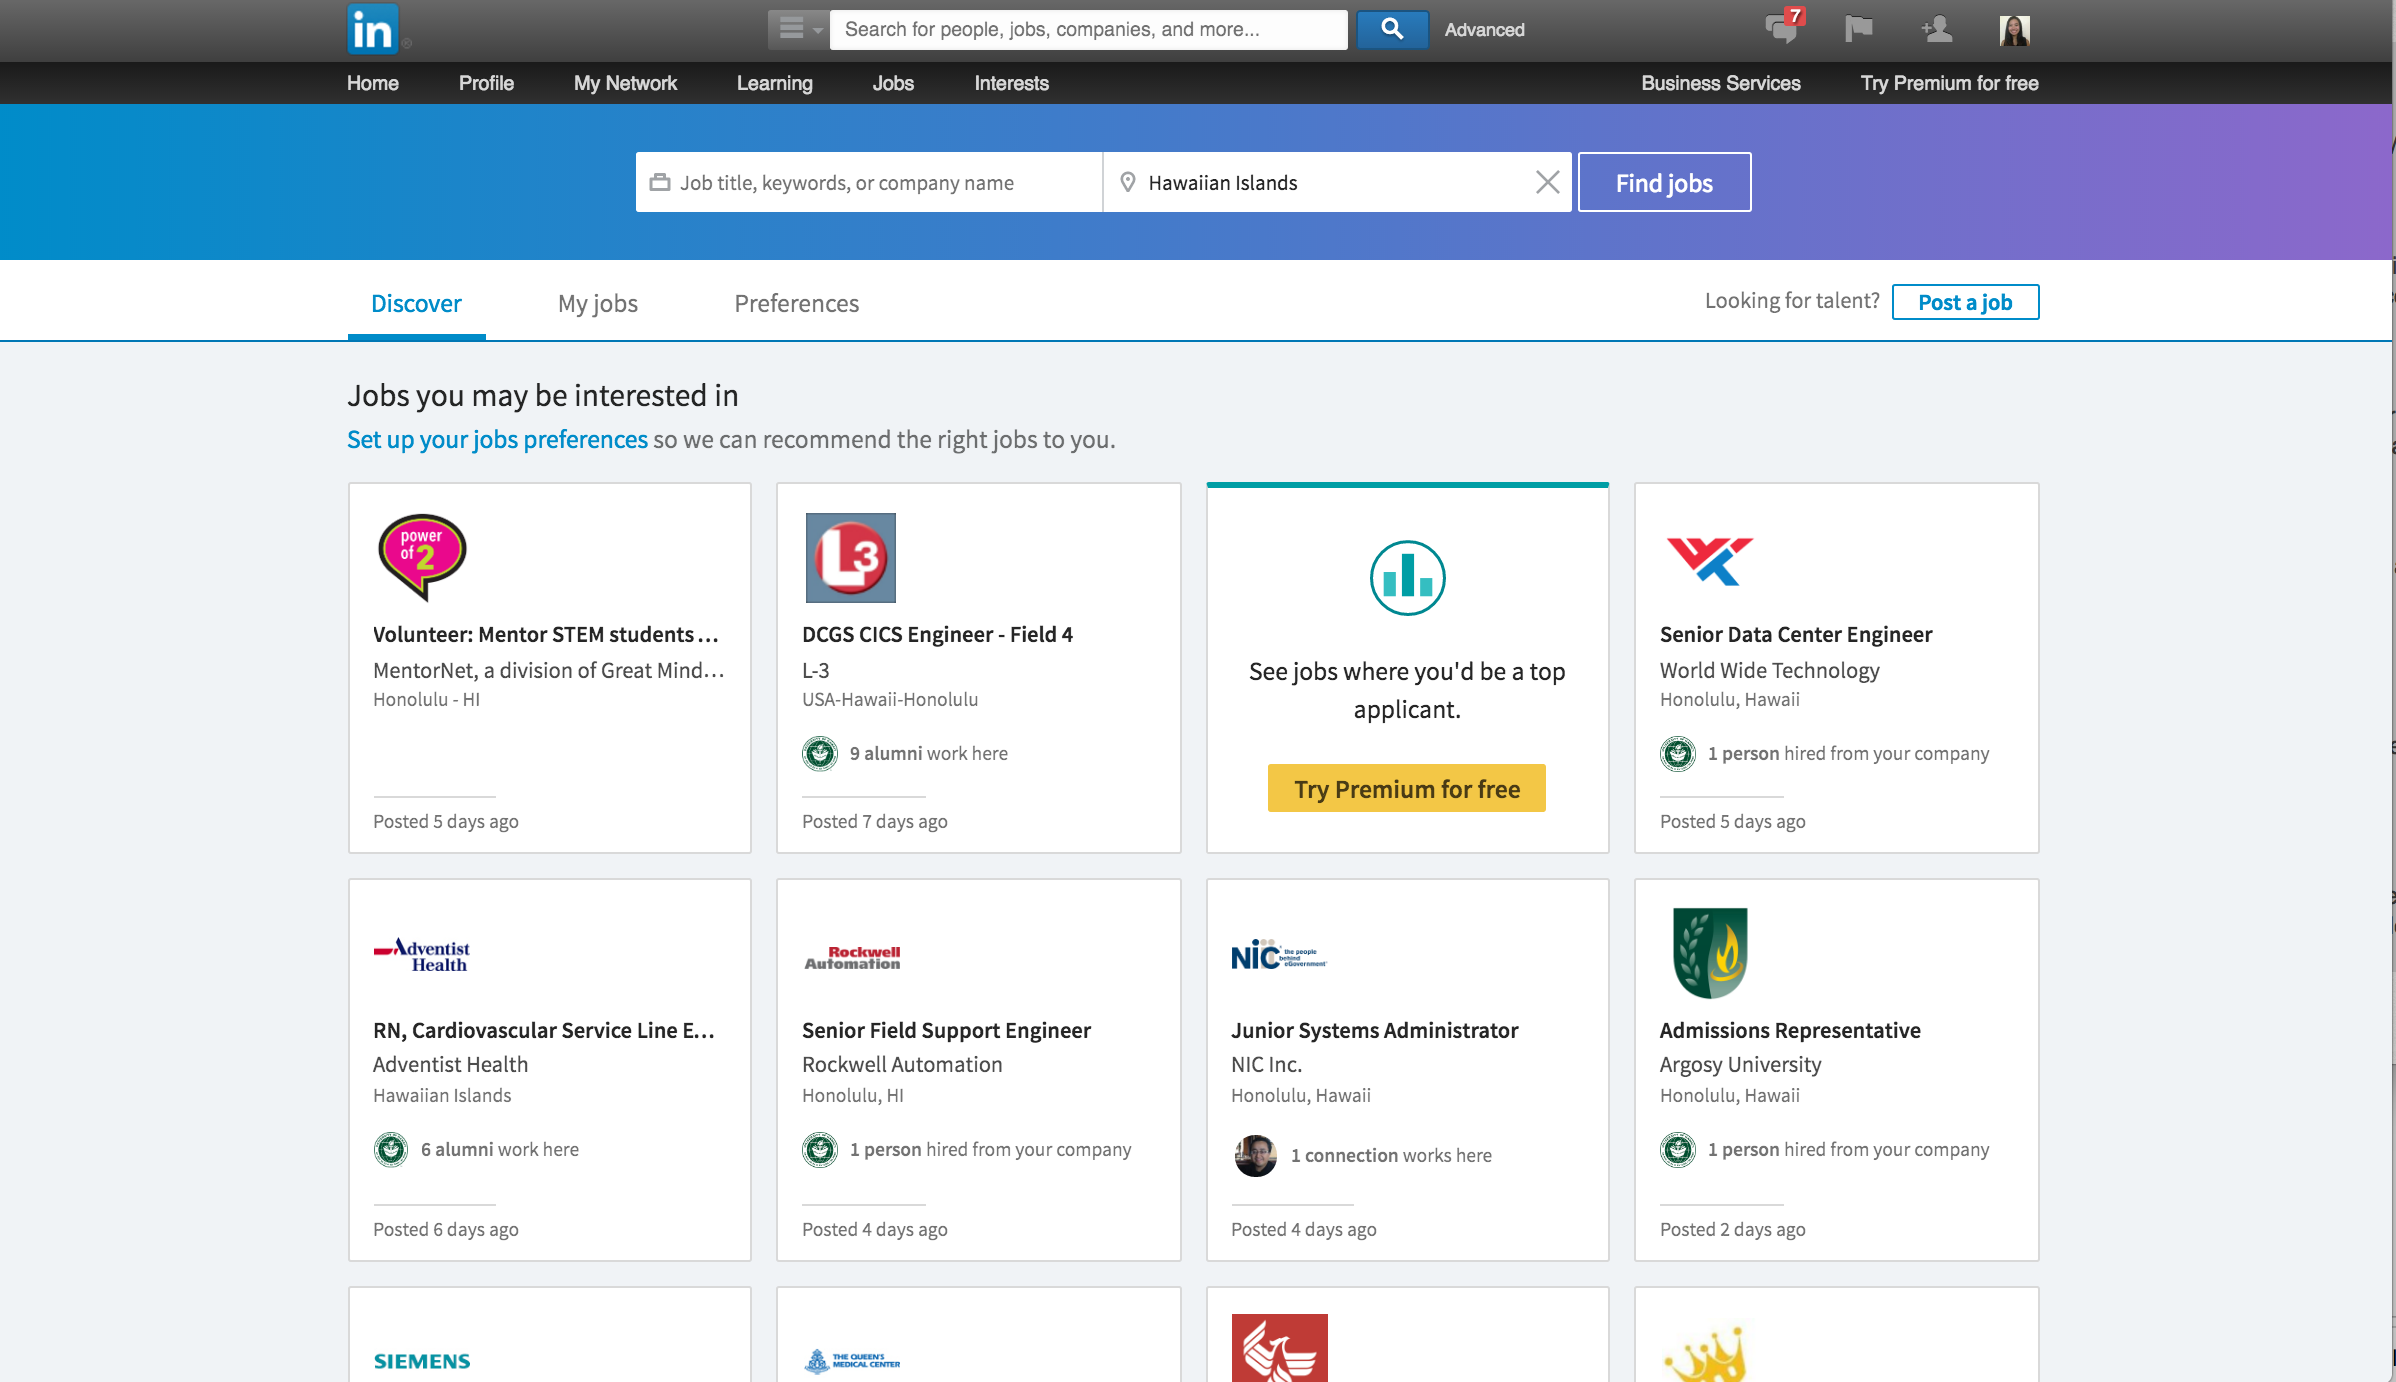
\includegraphics[width=1.0\textwidth]{linkedin_jobs}
\caption{LinkedIn jobs page. \textit{Source: http://www.linkedin.com}}
\end{figure}
\subsubsection{Jobs}
Jobs on LinkedIn automatically suggest jobs for users based off the information on their profile. Jobs can also be searched for using keywords such as job title, company, and location. Users can set preferences to refine their automatic suggestions.

\begin{figure}[h]
\centering
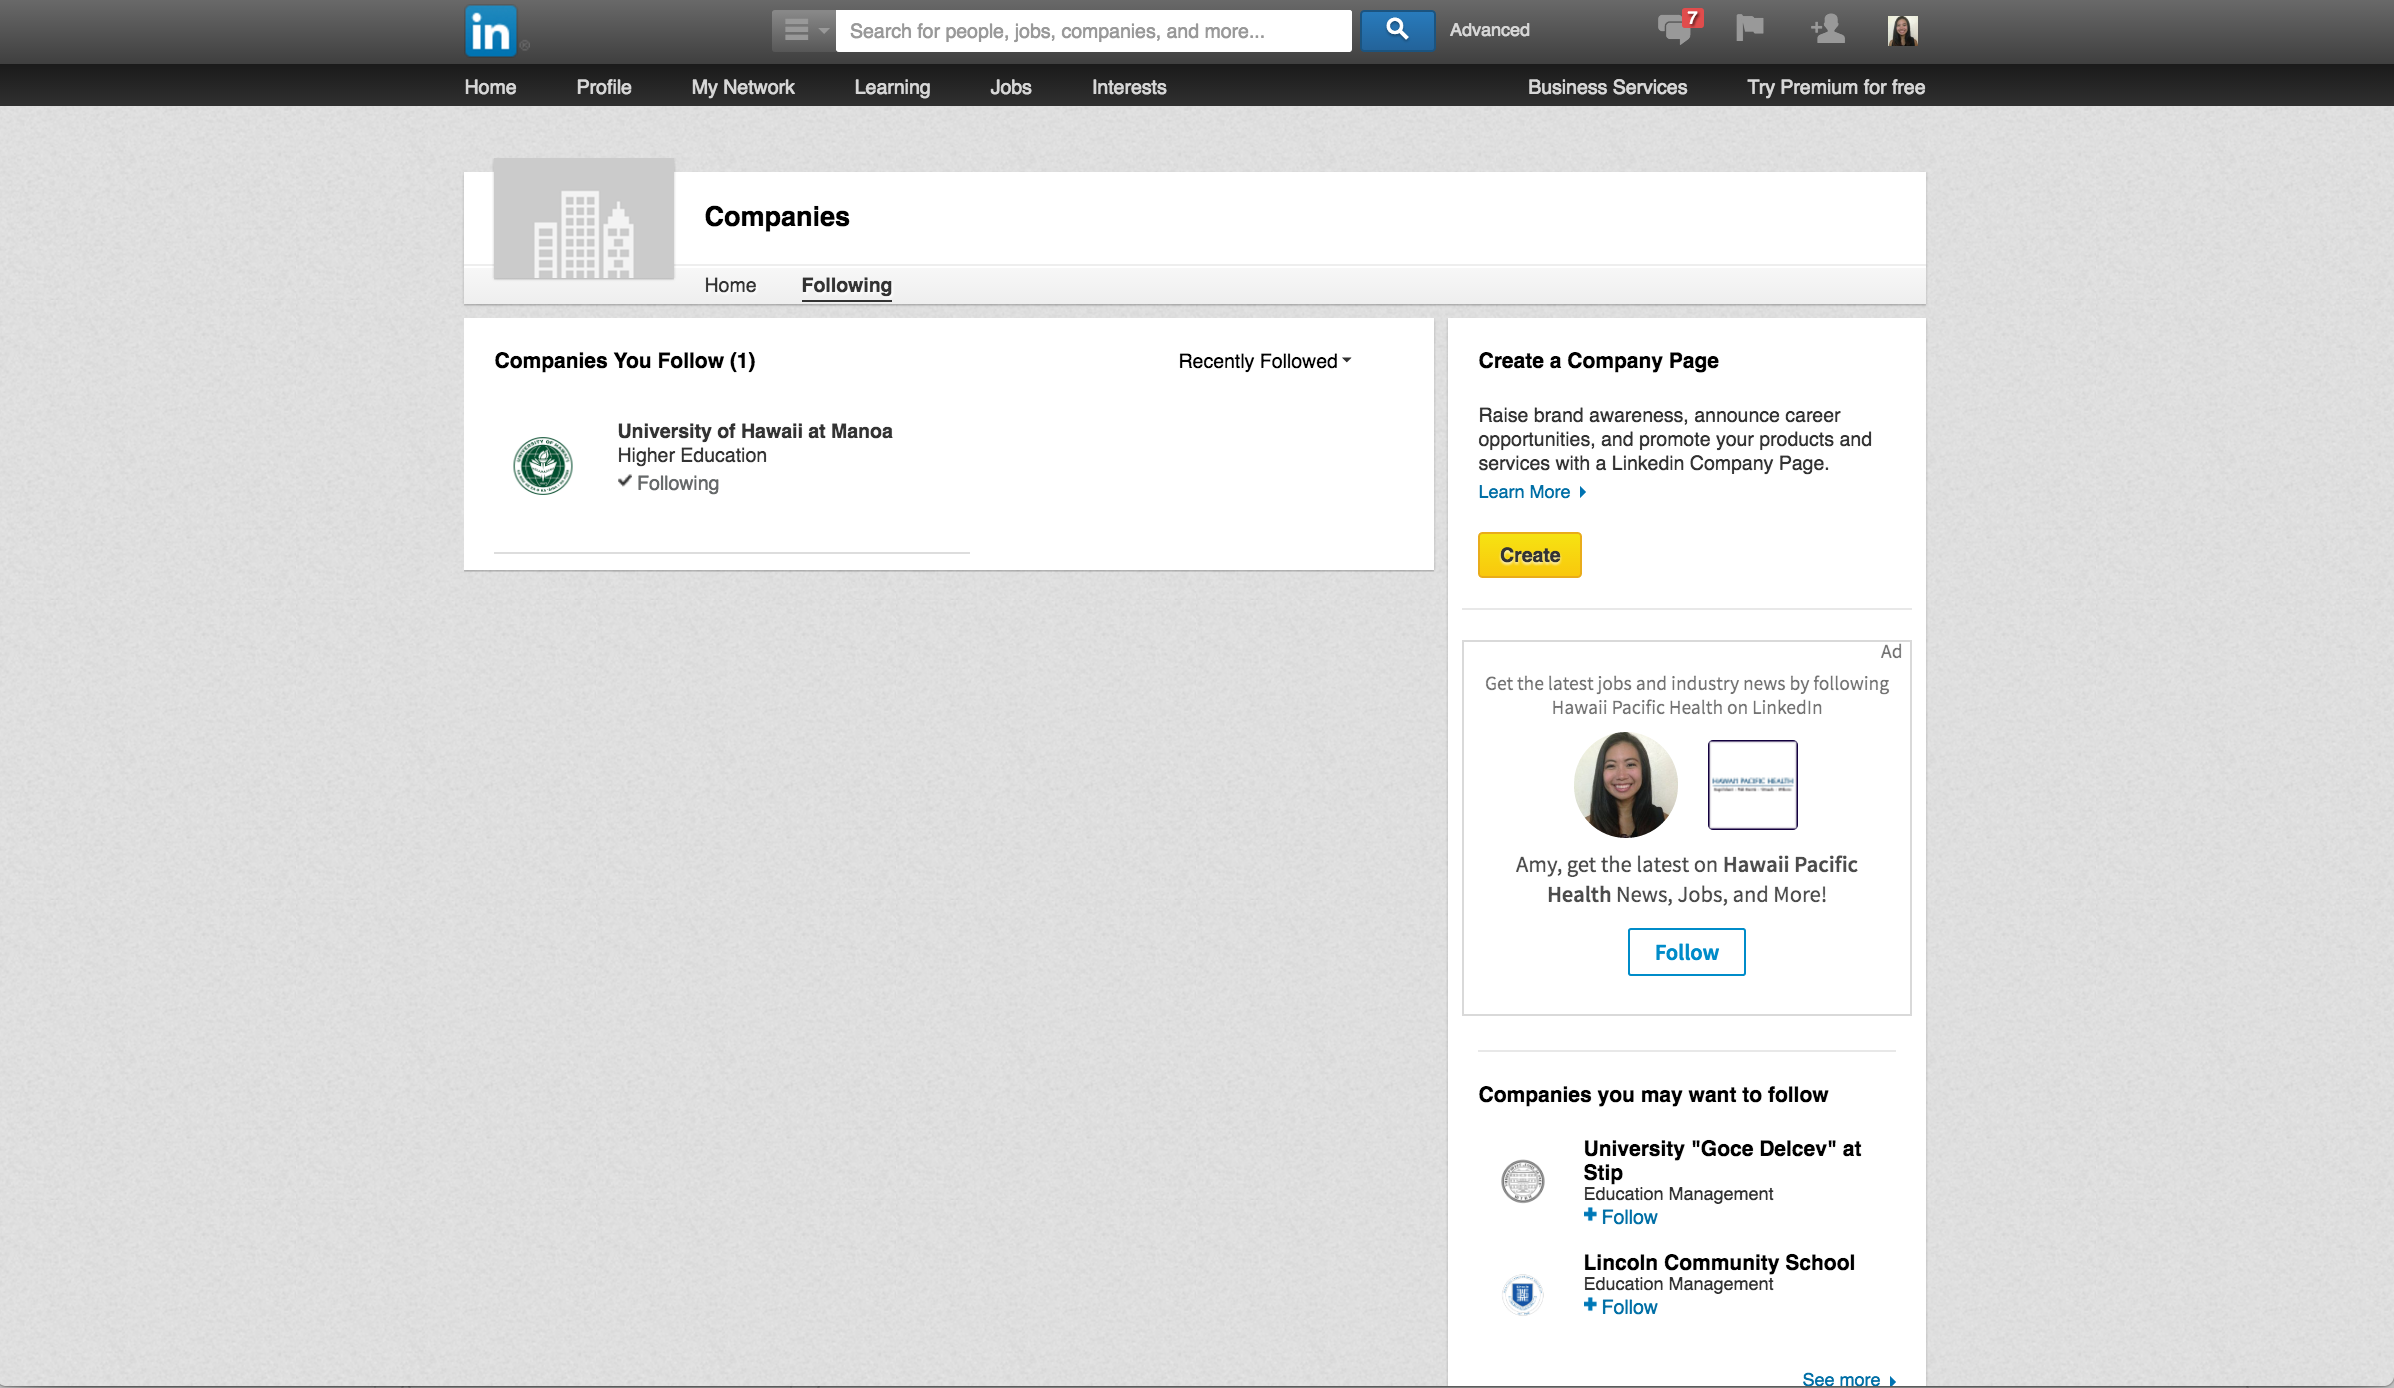
\includegraphics[width=1.0\textwidth]{linkedin_companies}
\caption{LinkedIn companies page in the Interests section. \textit{Source: http://www.linkedin.com}}
\end{figure}
\subsubsection{Interests}
In the Interests section, users can follow companies and groups based off their personal interests. There are also links to SlideShare and ProFinder, which offer services for creating professional presentations and hiring local freelancers, respectively.

\subsubsection{LinkedIn and Academic/Professional/Social Engagement}
LinkedIn is a large global professional network. The more people it reaches, and the more diverse it becomes, the more successful it will be. This works on a large scale. Due to this, LinkedIn inherently fails to provide the intimate support of a smaller and more personal community. It is easy to become overwhelmed with the breadth of LinkedIn, but if there were a place that offered a smaller and more specific community with a lot more depth, people would be able to create stronger and deeper connections (with the trade-off being having less connections overall). For students who have not graduated college yet, having strong connections with the people they are surrounded by (colleagues, professors, alumni, etc.) is arguably more important than having many loose connections with a wider network. This is not to say one type of network is better than the other--but for students, the support they need will come from the smaller and stronger network. 

\subsection{TechHui}
The TechHui page describes itself as being ``Hawaii's Technology Community." The TechHui site has ten main sections: Profile, Members, Events, Forum, Groups, Photos, Videos, Blogs, Directory, and Coders.

\begin{figure}[h]
\centering
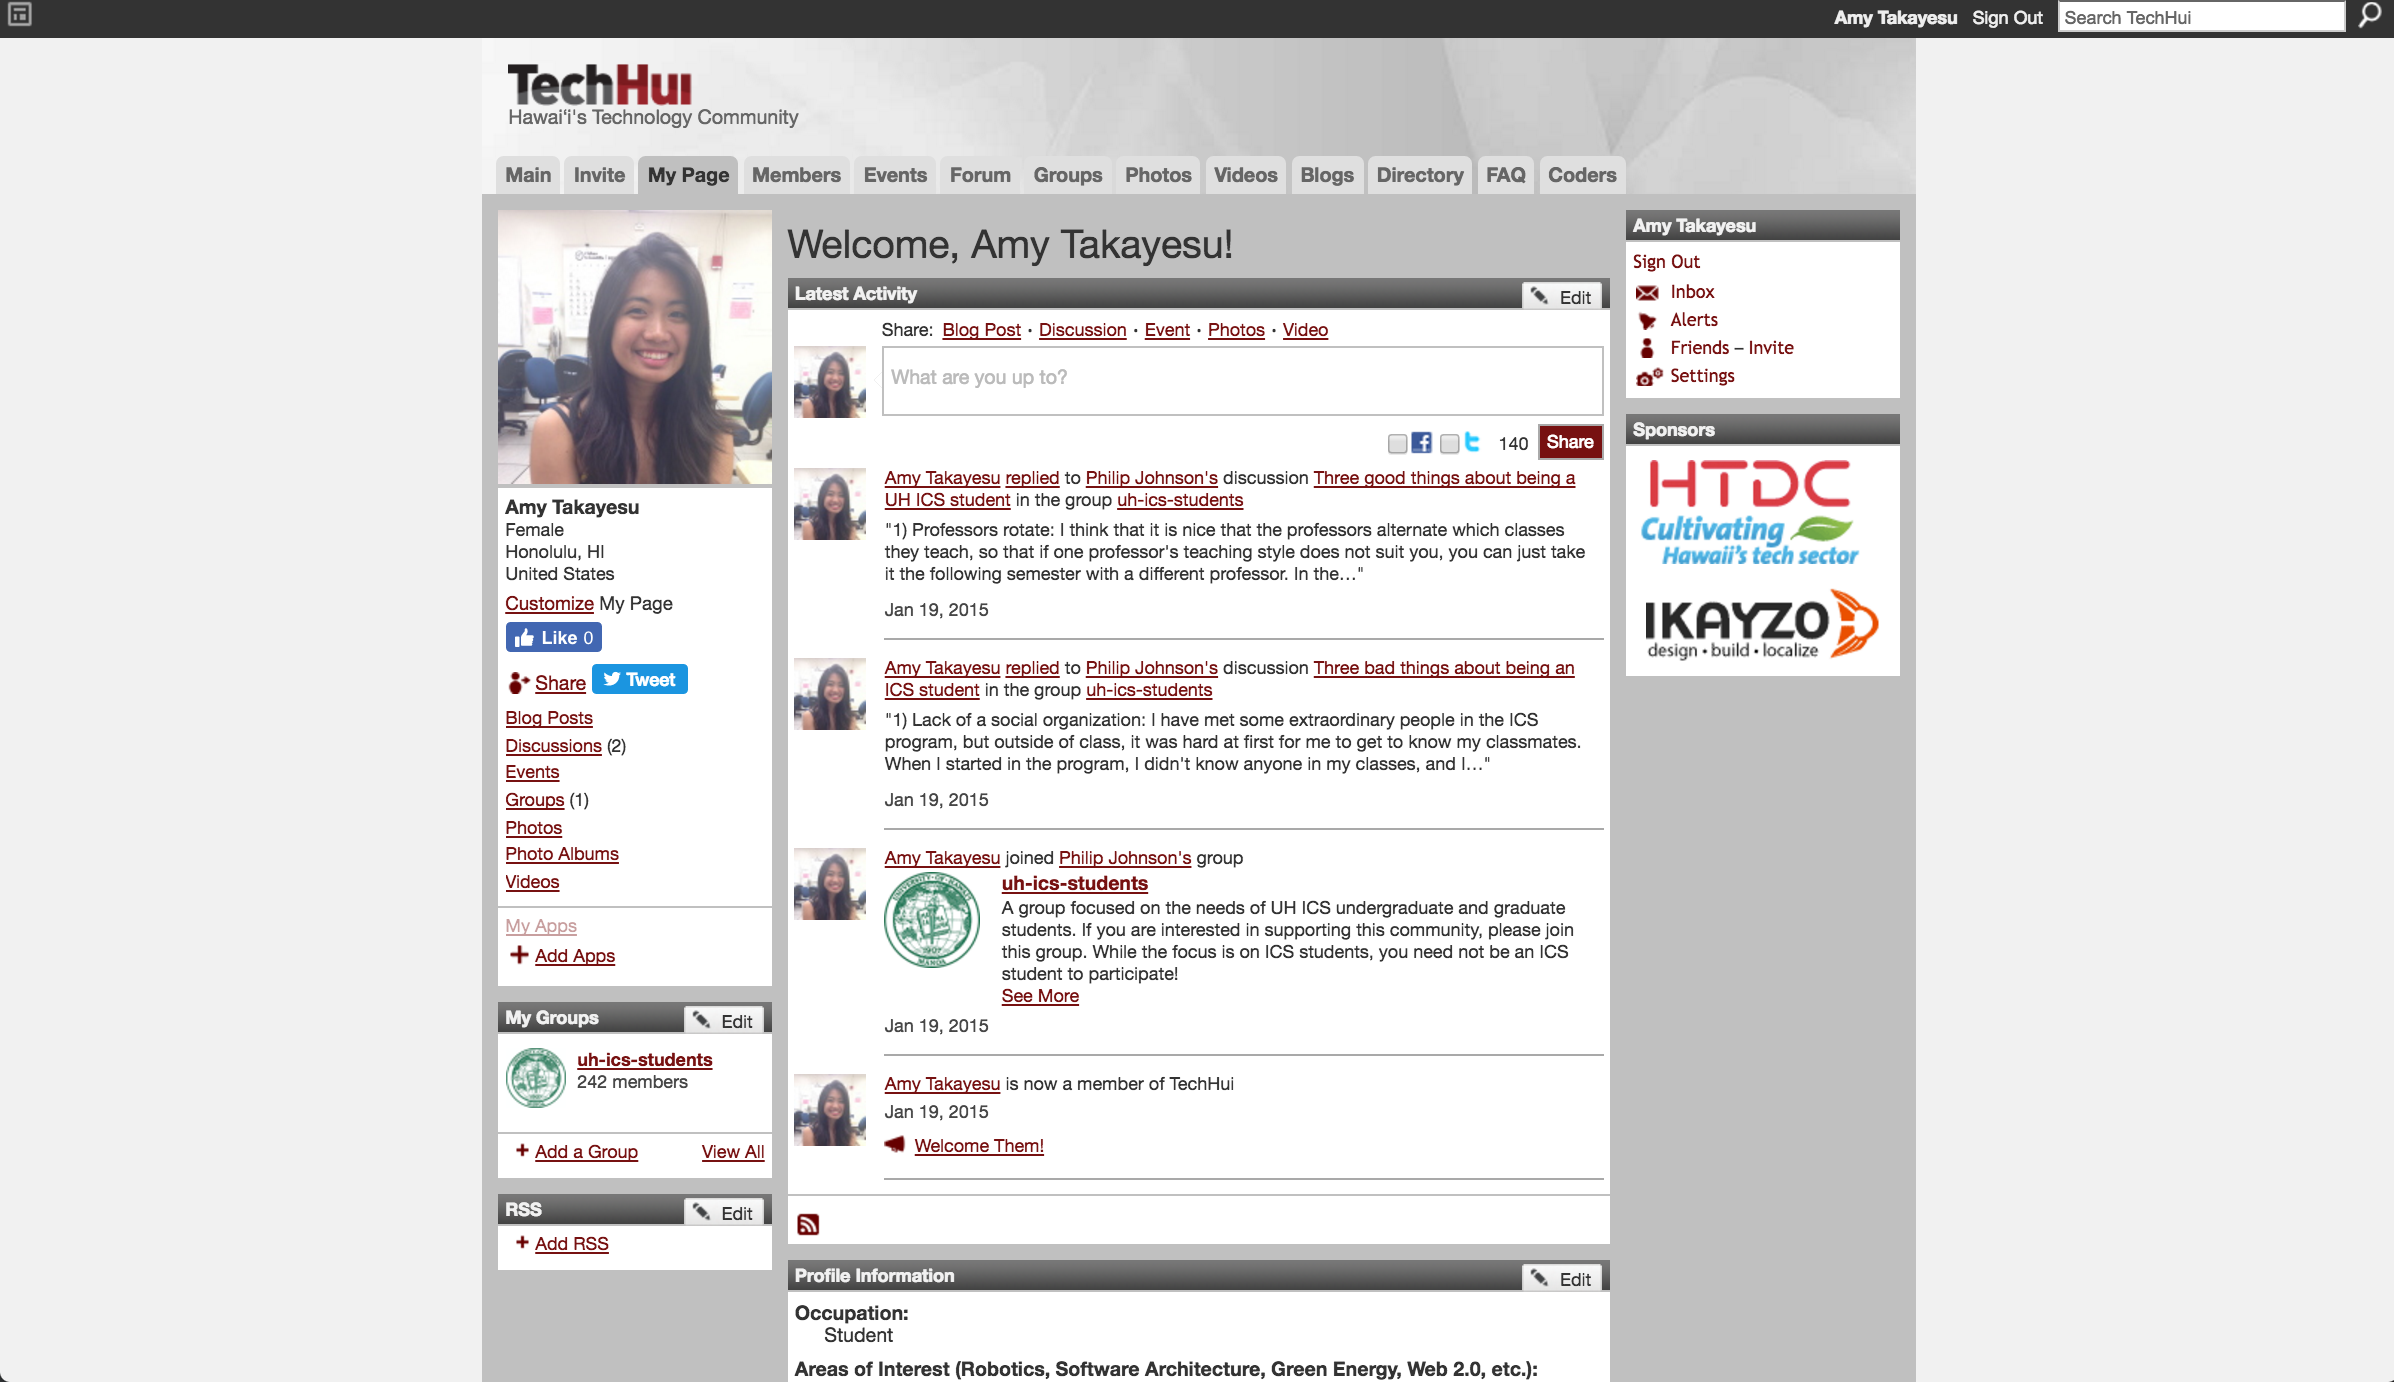
\includegraphics[width=1.0\textwidth]{techhui_profile}
\caption{TechHui profile page. \textit{Source: http://www.techhui.com}}
\end{figure}
\subsubsection{Profile}
Each user has a profile page which contains information such as a name, profile picture, occupation, areas of interest, software language proficiency and interests, and recent activity.

\begin{figure}[h]
\centering
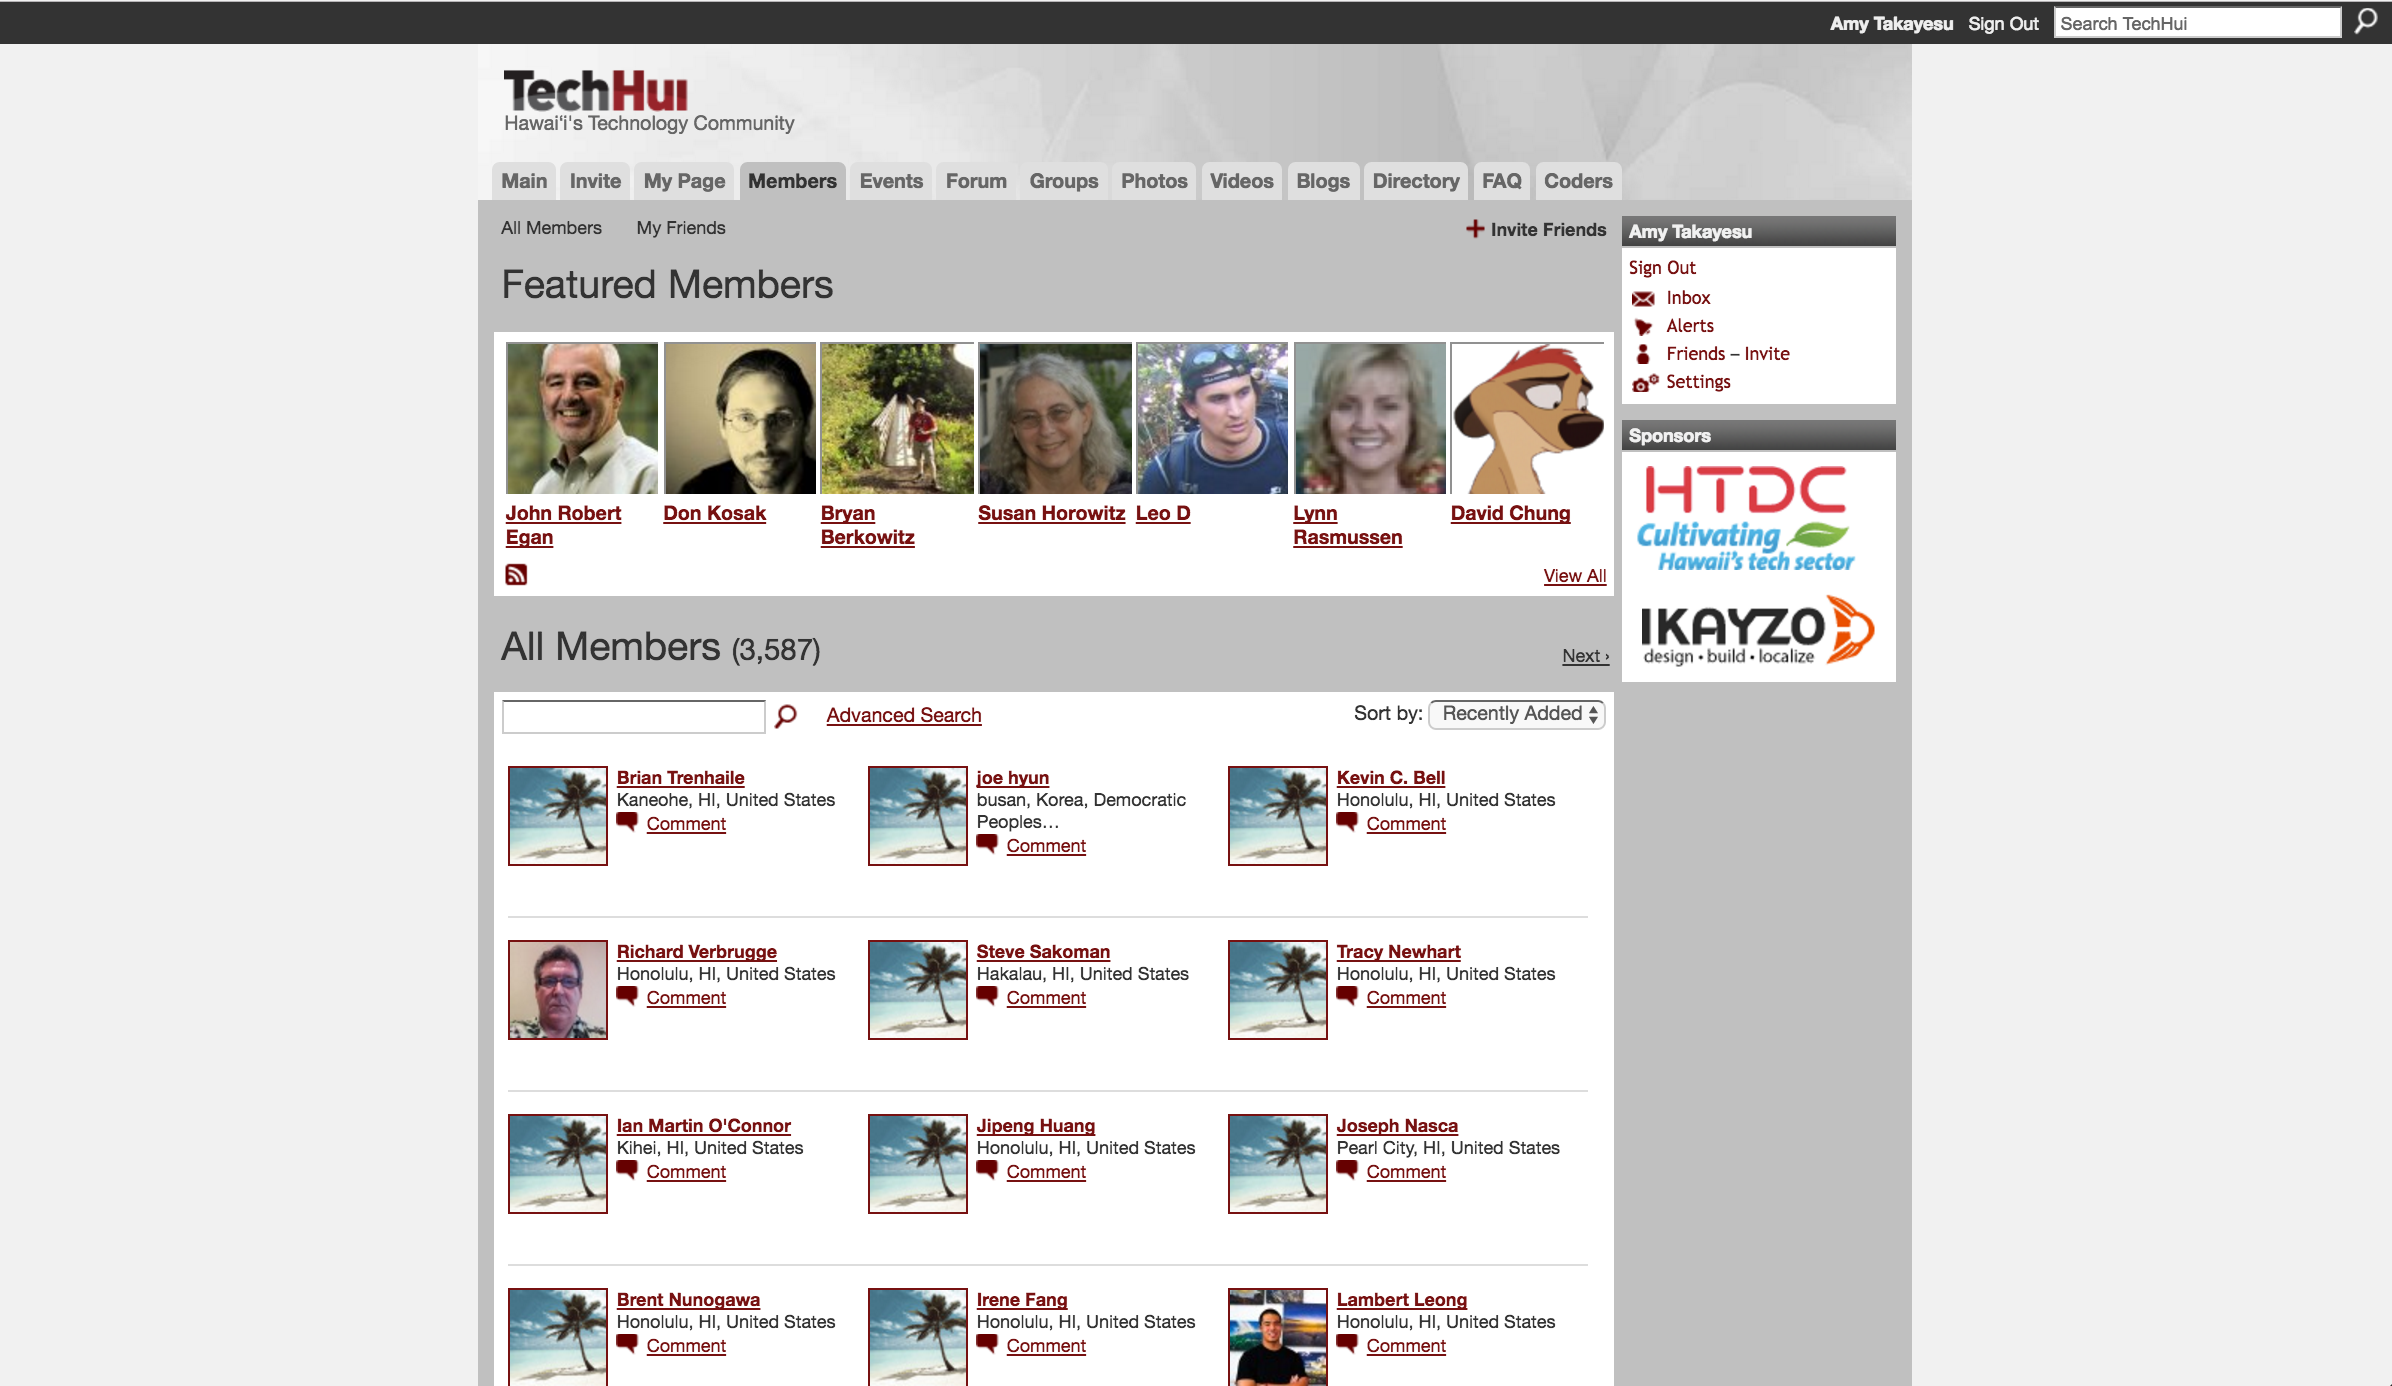
\includegraphics[width=1.0\textwidth]{techhui_members}
\caption{TechHui members page. \textit{Source: http://www.techhui.com}}
\end{figure}
\subsubsection{Members}
The members page lists all members, including a section at the top for featured members. Each member is listed by their name, with their profile picture and location. Through this page, users can communicate with other users by commenting on other user's profile pages.

\begin{figure}[h]
\centering
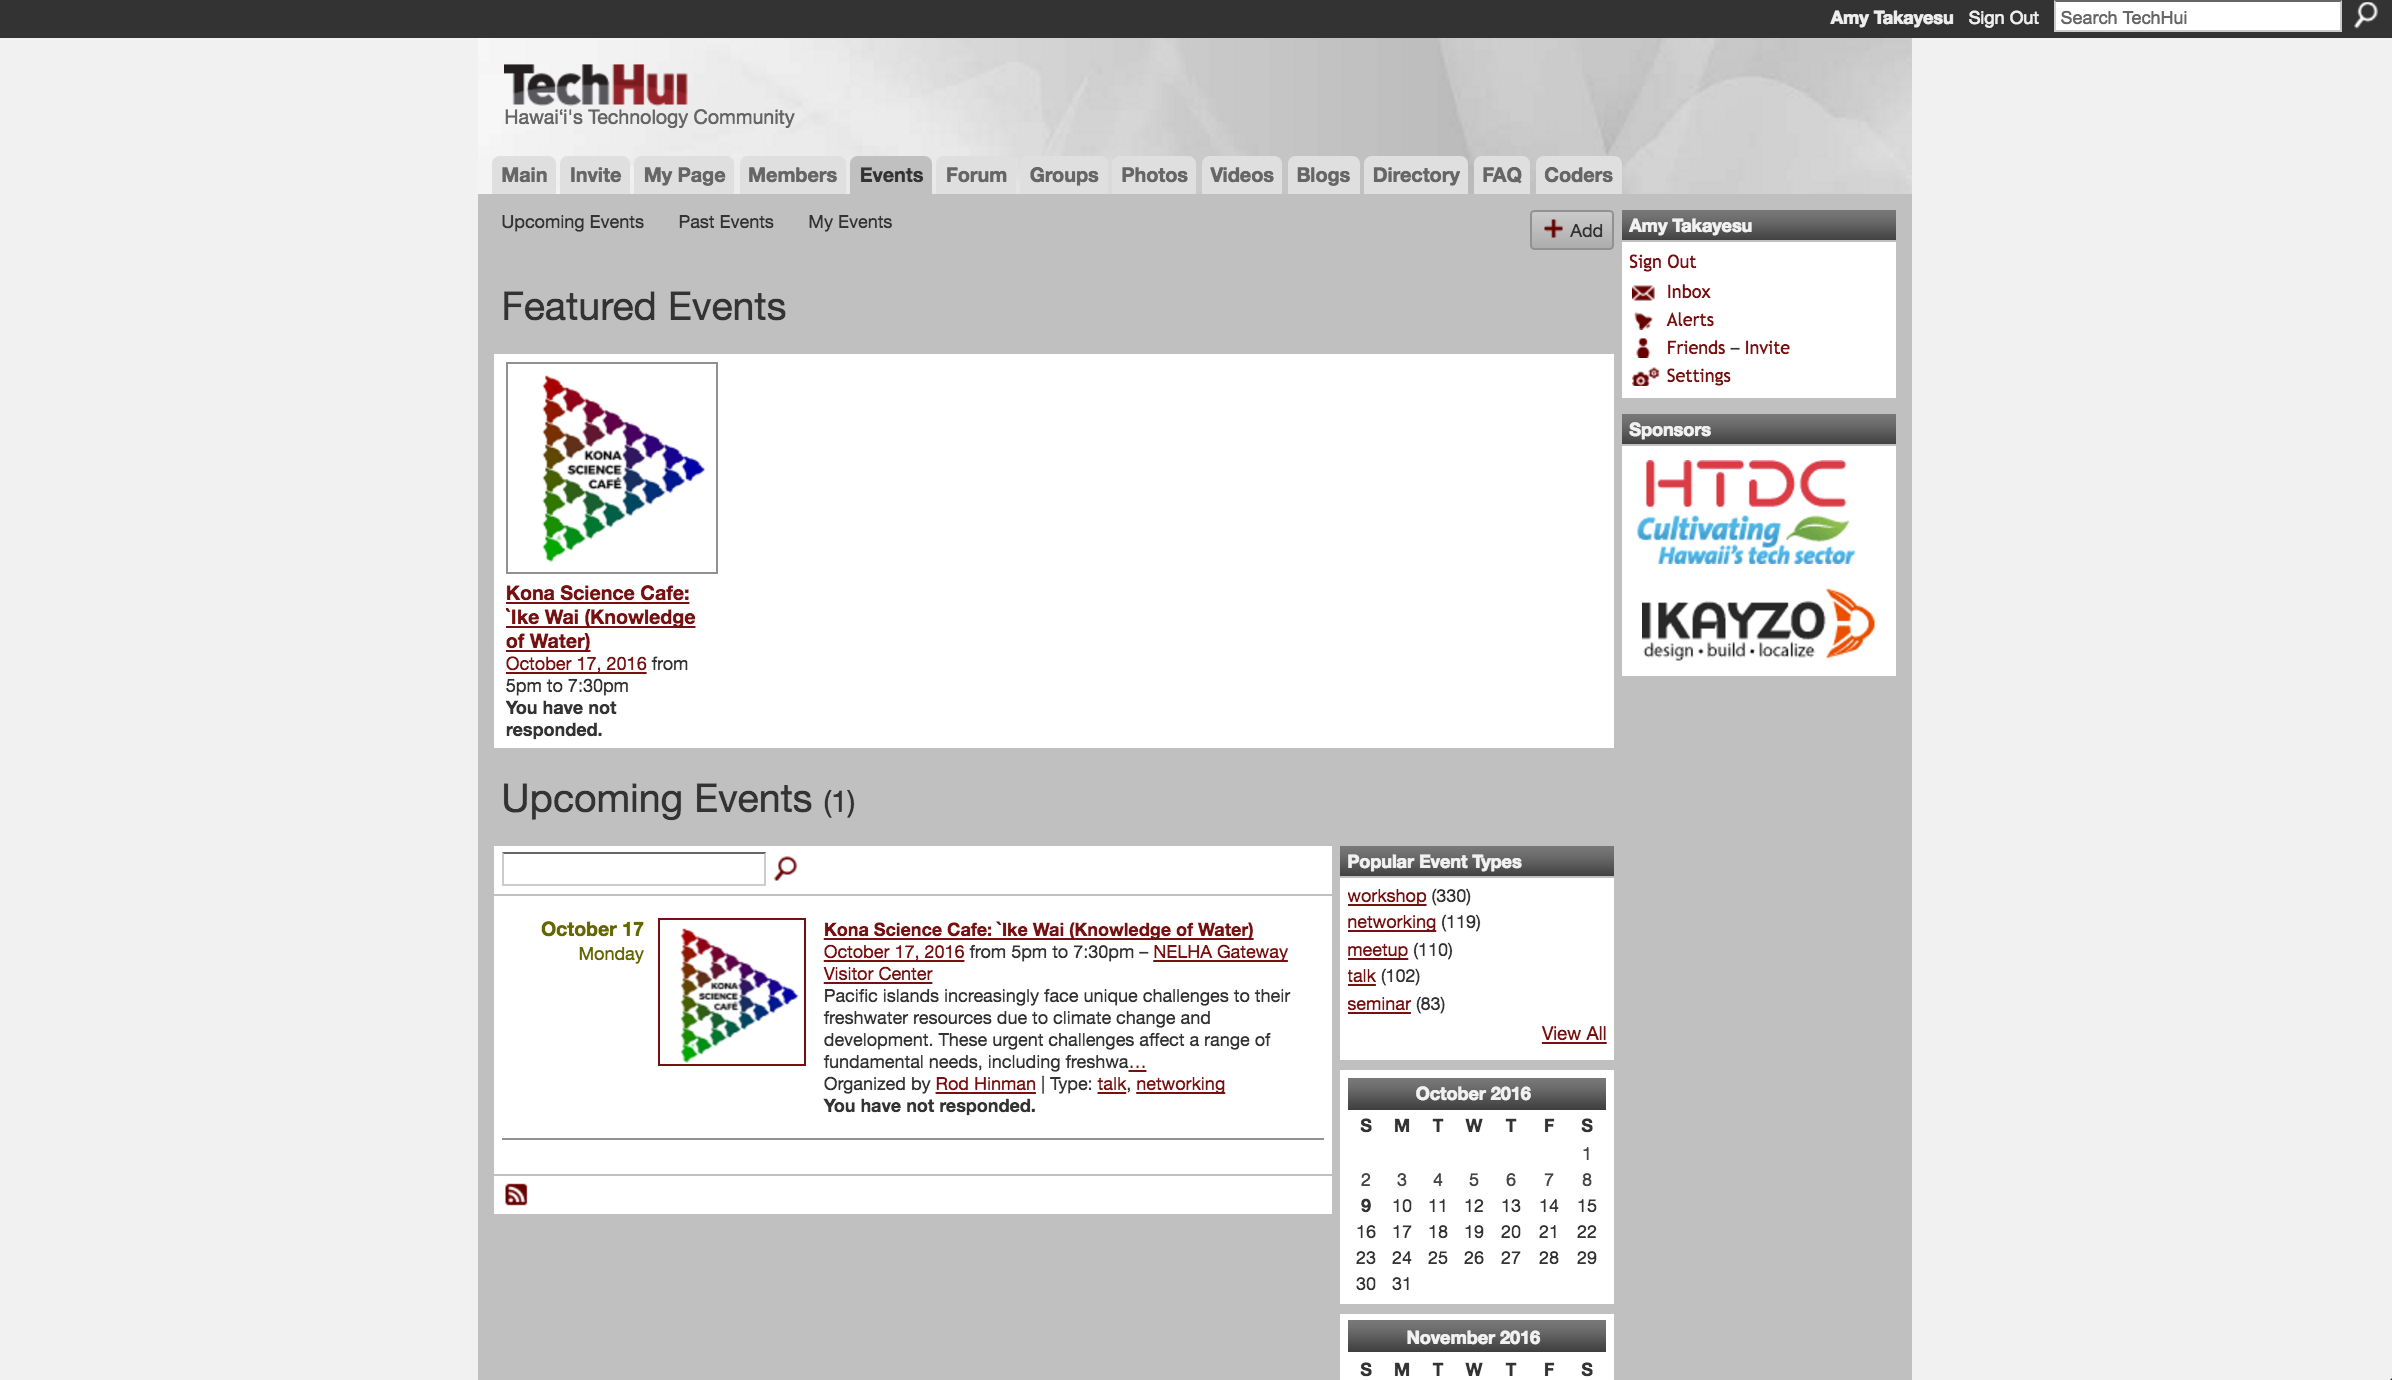
\includegraphics[width=1.0\textwidth]{techhui_events}
\caption{TechHui events page. \textit{Source: http://www.techhui.com}}
\end{figure}
\subsubsection{Events}
The events page lists upcoming events and featured events. The event snippets include an imagine, a name, a time and date, a location, the name of the organizer, the type of event, and a brief description of the event. Users can click on these snippets to go to an event page, which includes more detailed information and allows users to respond to events with ``will attend", ``might attend" and ``will not attend." 

\begin{figure}[h]
\centering
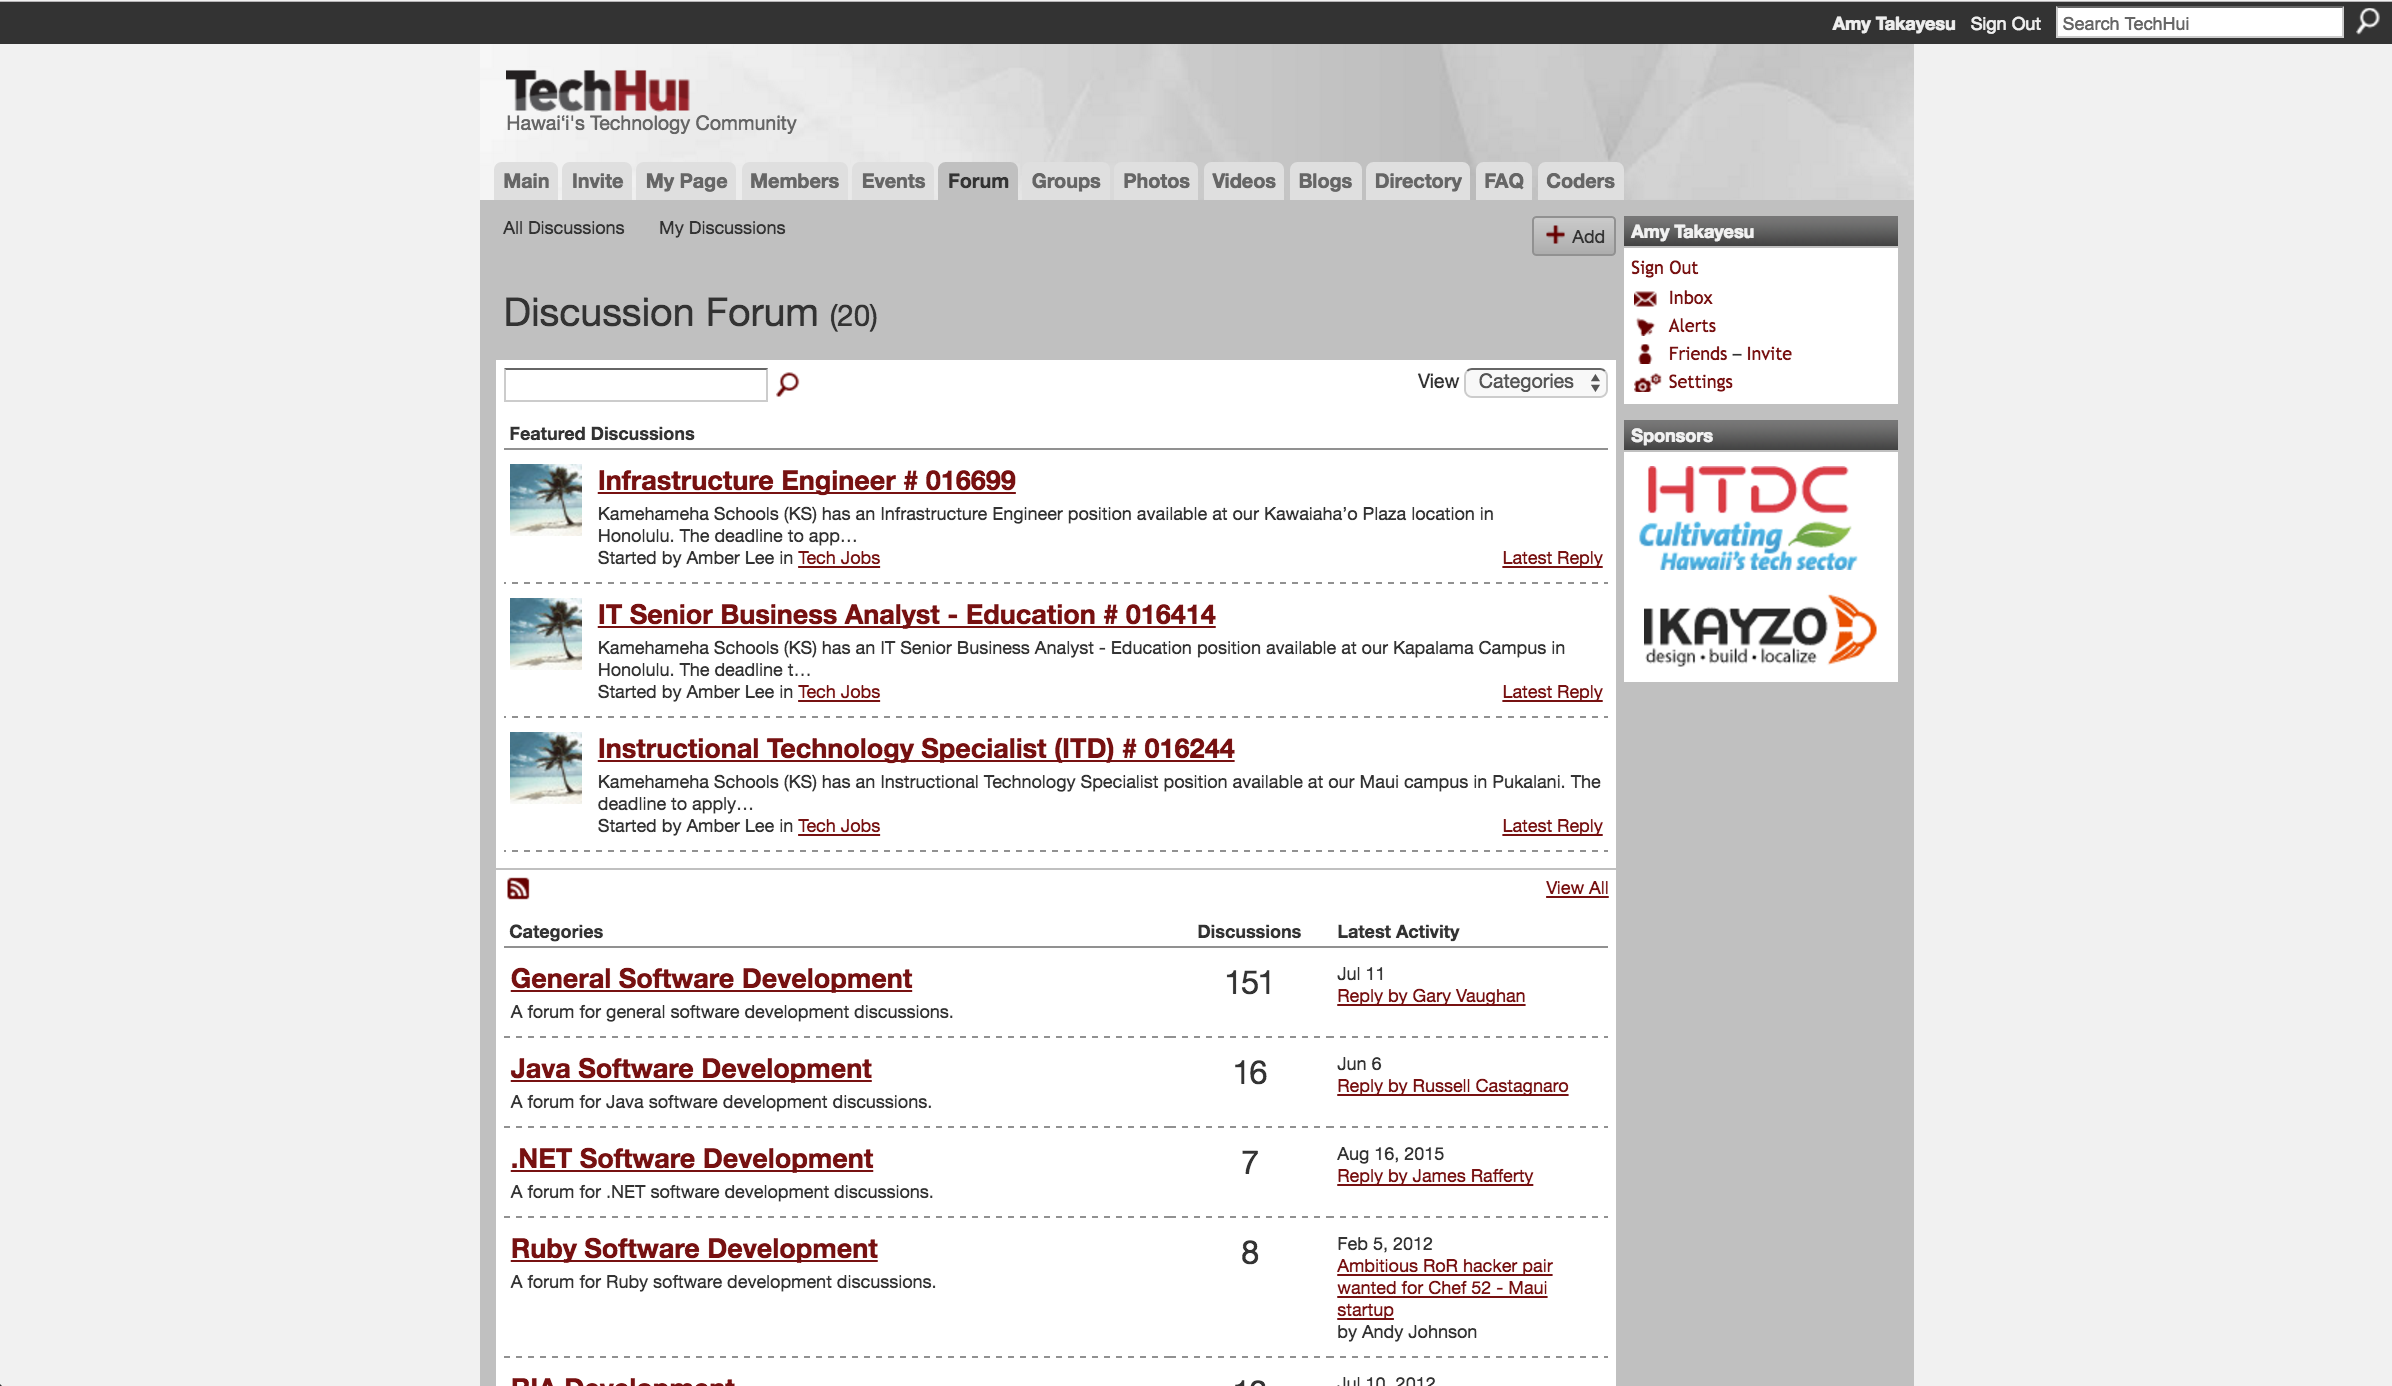
\includegraphics[width=1.0\textwidth]{techhui_forum}
\caption{TechHui forum page. \textit{Source: http://www.techhui.com}}
\end{figure}
\subsubsection{Forum}
The forum page includes a list of technology related categories, which can be clicked on to access a list of related forums. It also includes some featured forums at the top. Some of these categories include ``General Software Development", ``Java Software Development", ``Funding Technology Startups", ``Software Design Patterns", ``Tech Jobs", ``Tech Resumes", ``Web Design", ``Tech Humor" and more. Users can both start discussion forums and respond to other users' forums. 

\begin{figure}[h]
\centering
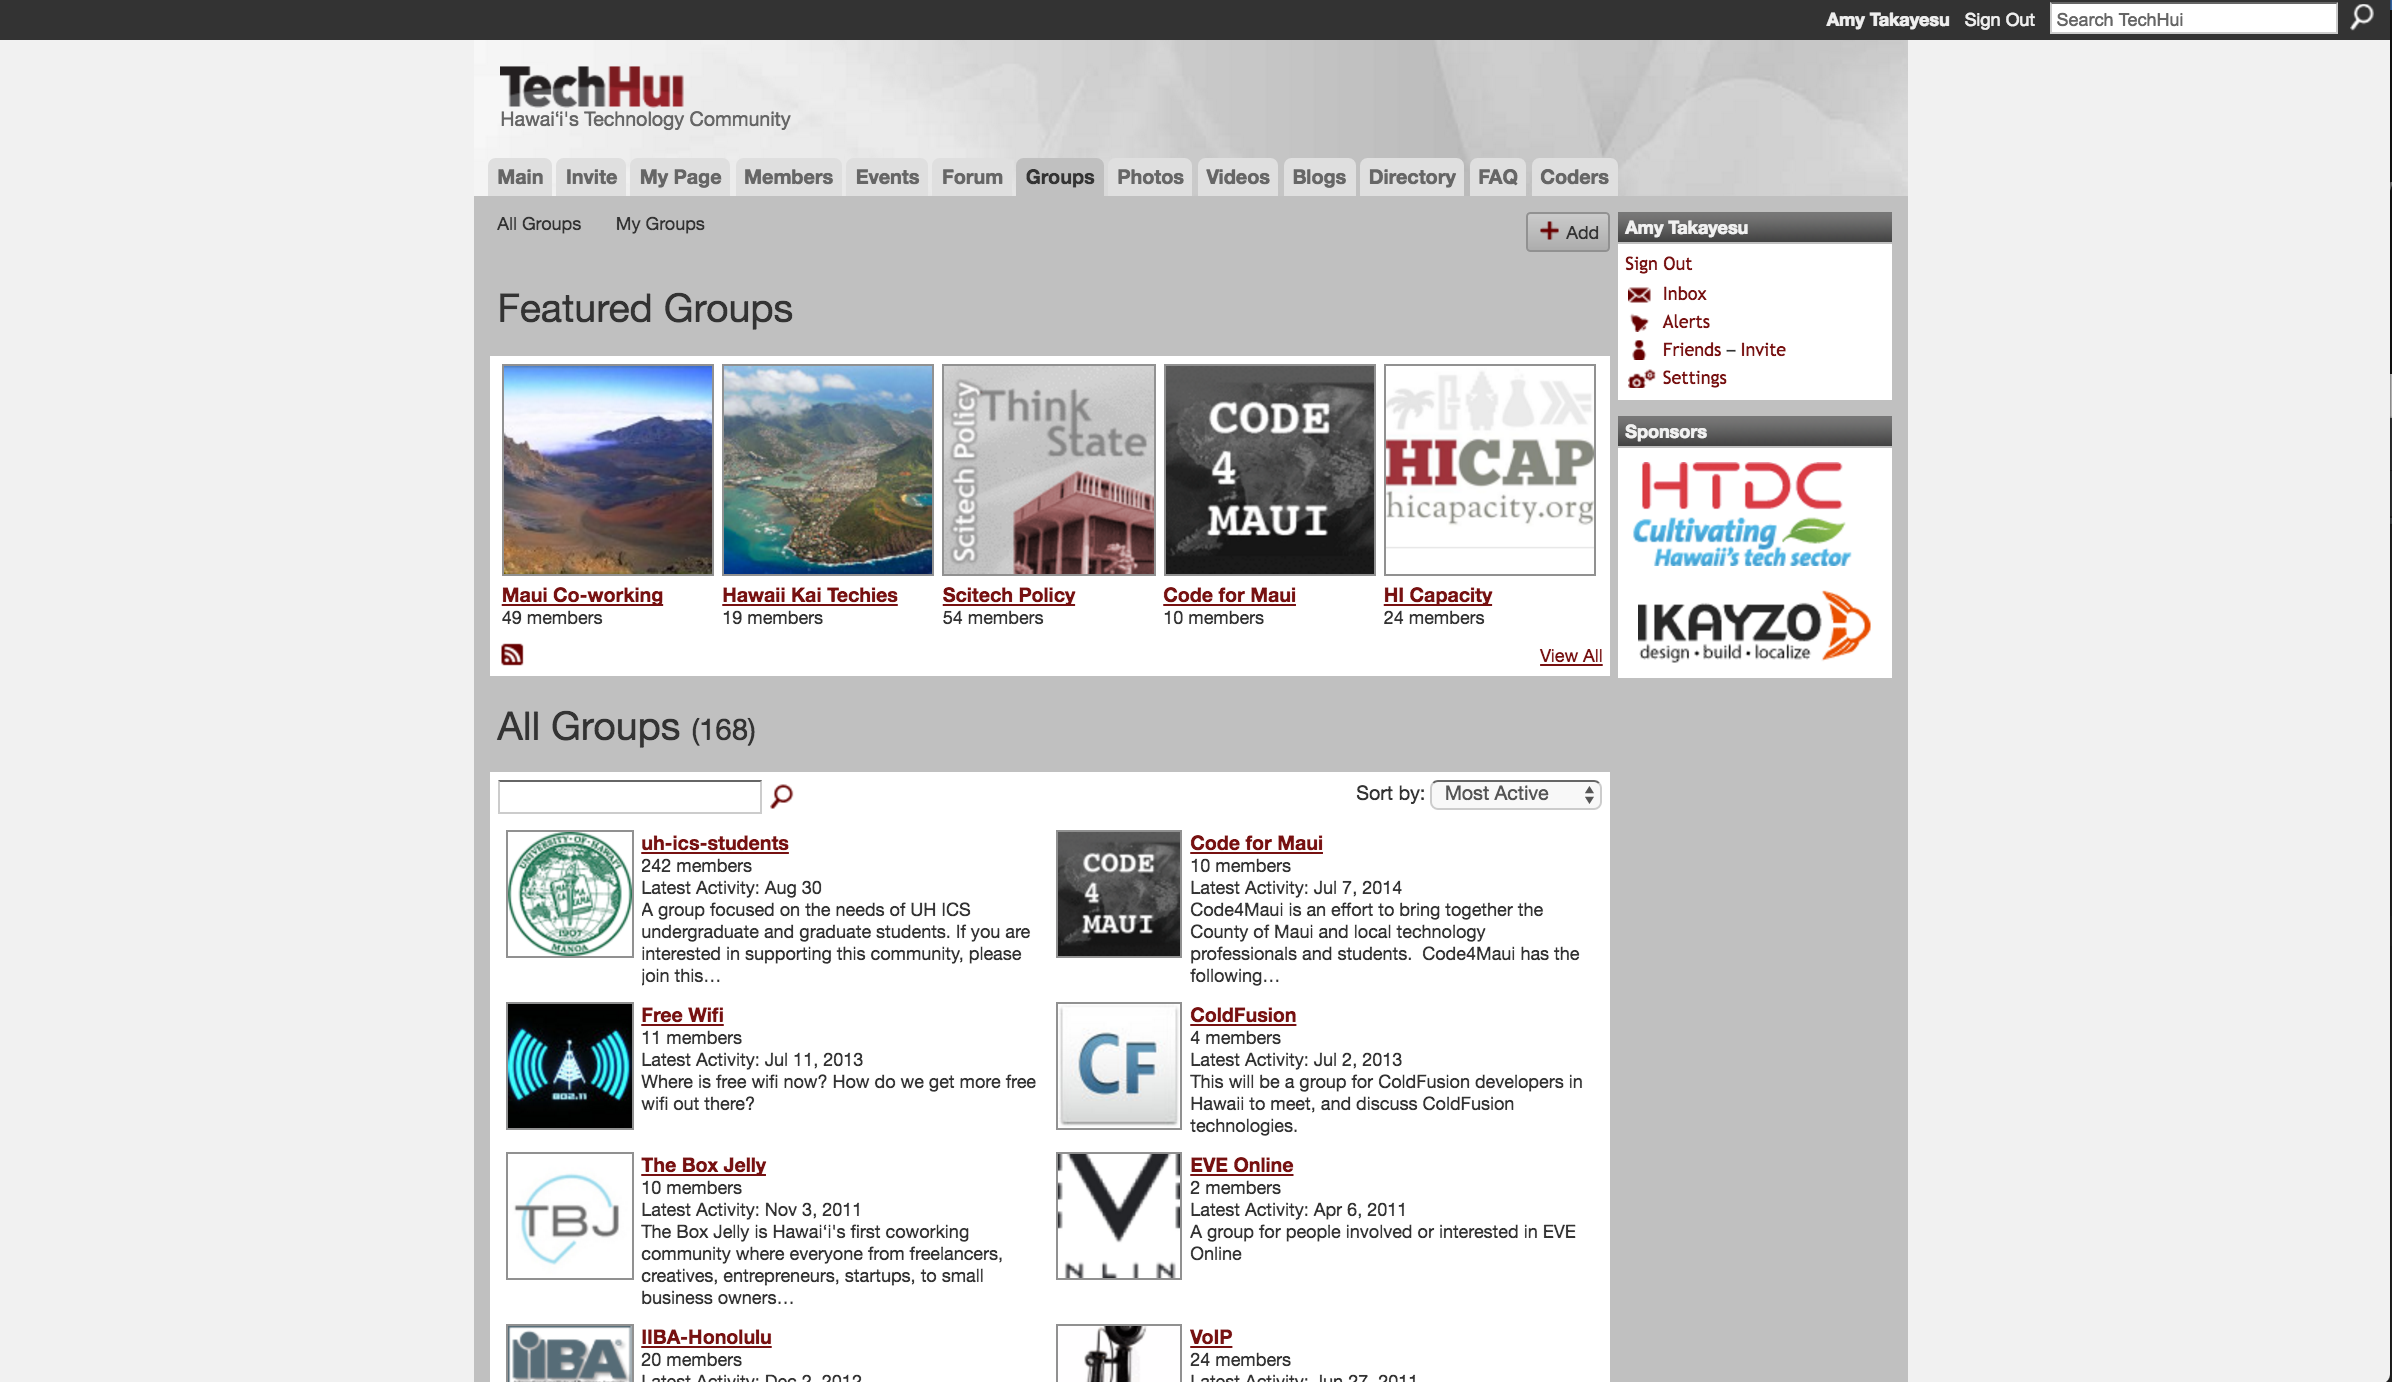
\includegraphics[width=1.0\textwidth]{techhui_groups}
\caption{TechHui groups page. \textit{Source: http://www.techhui.com}}
\end{figure}
\subsubsection{Groups}
There are many different groups listed on this page, including some featured groups. Each group snippet has an image, a name, the amount of members in the group, the date of the group's latest activity, and a brief description of the group. Users can click on these snippets to learn more about the group and to join the group as well. Once in the group, users can participate in commenting on the group wall and creating and responding to group discussion forums. 

\begin{figure}[h]
\centering
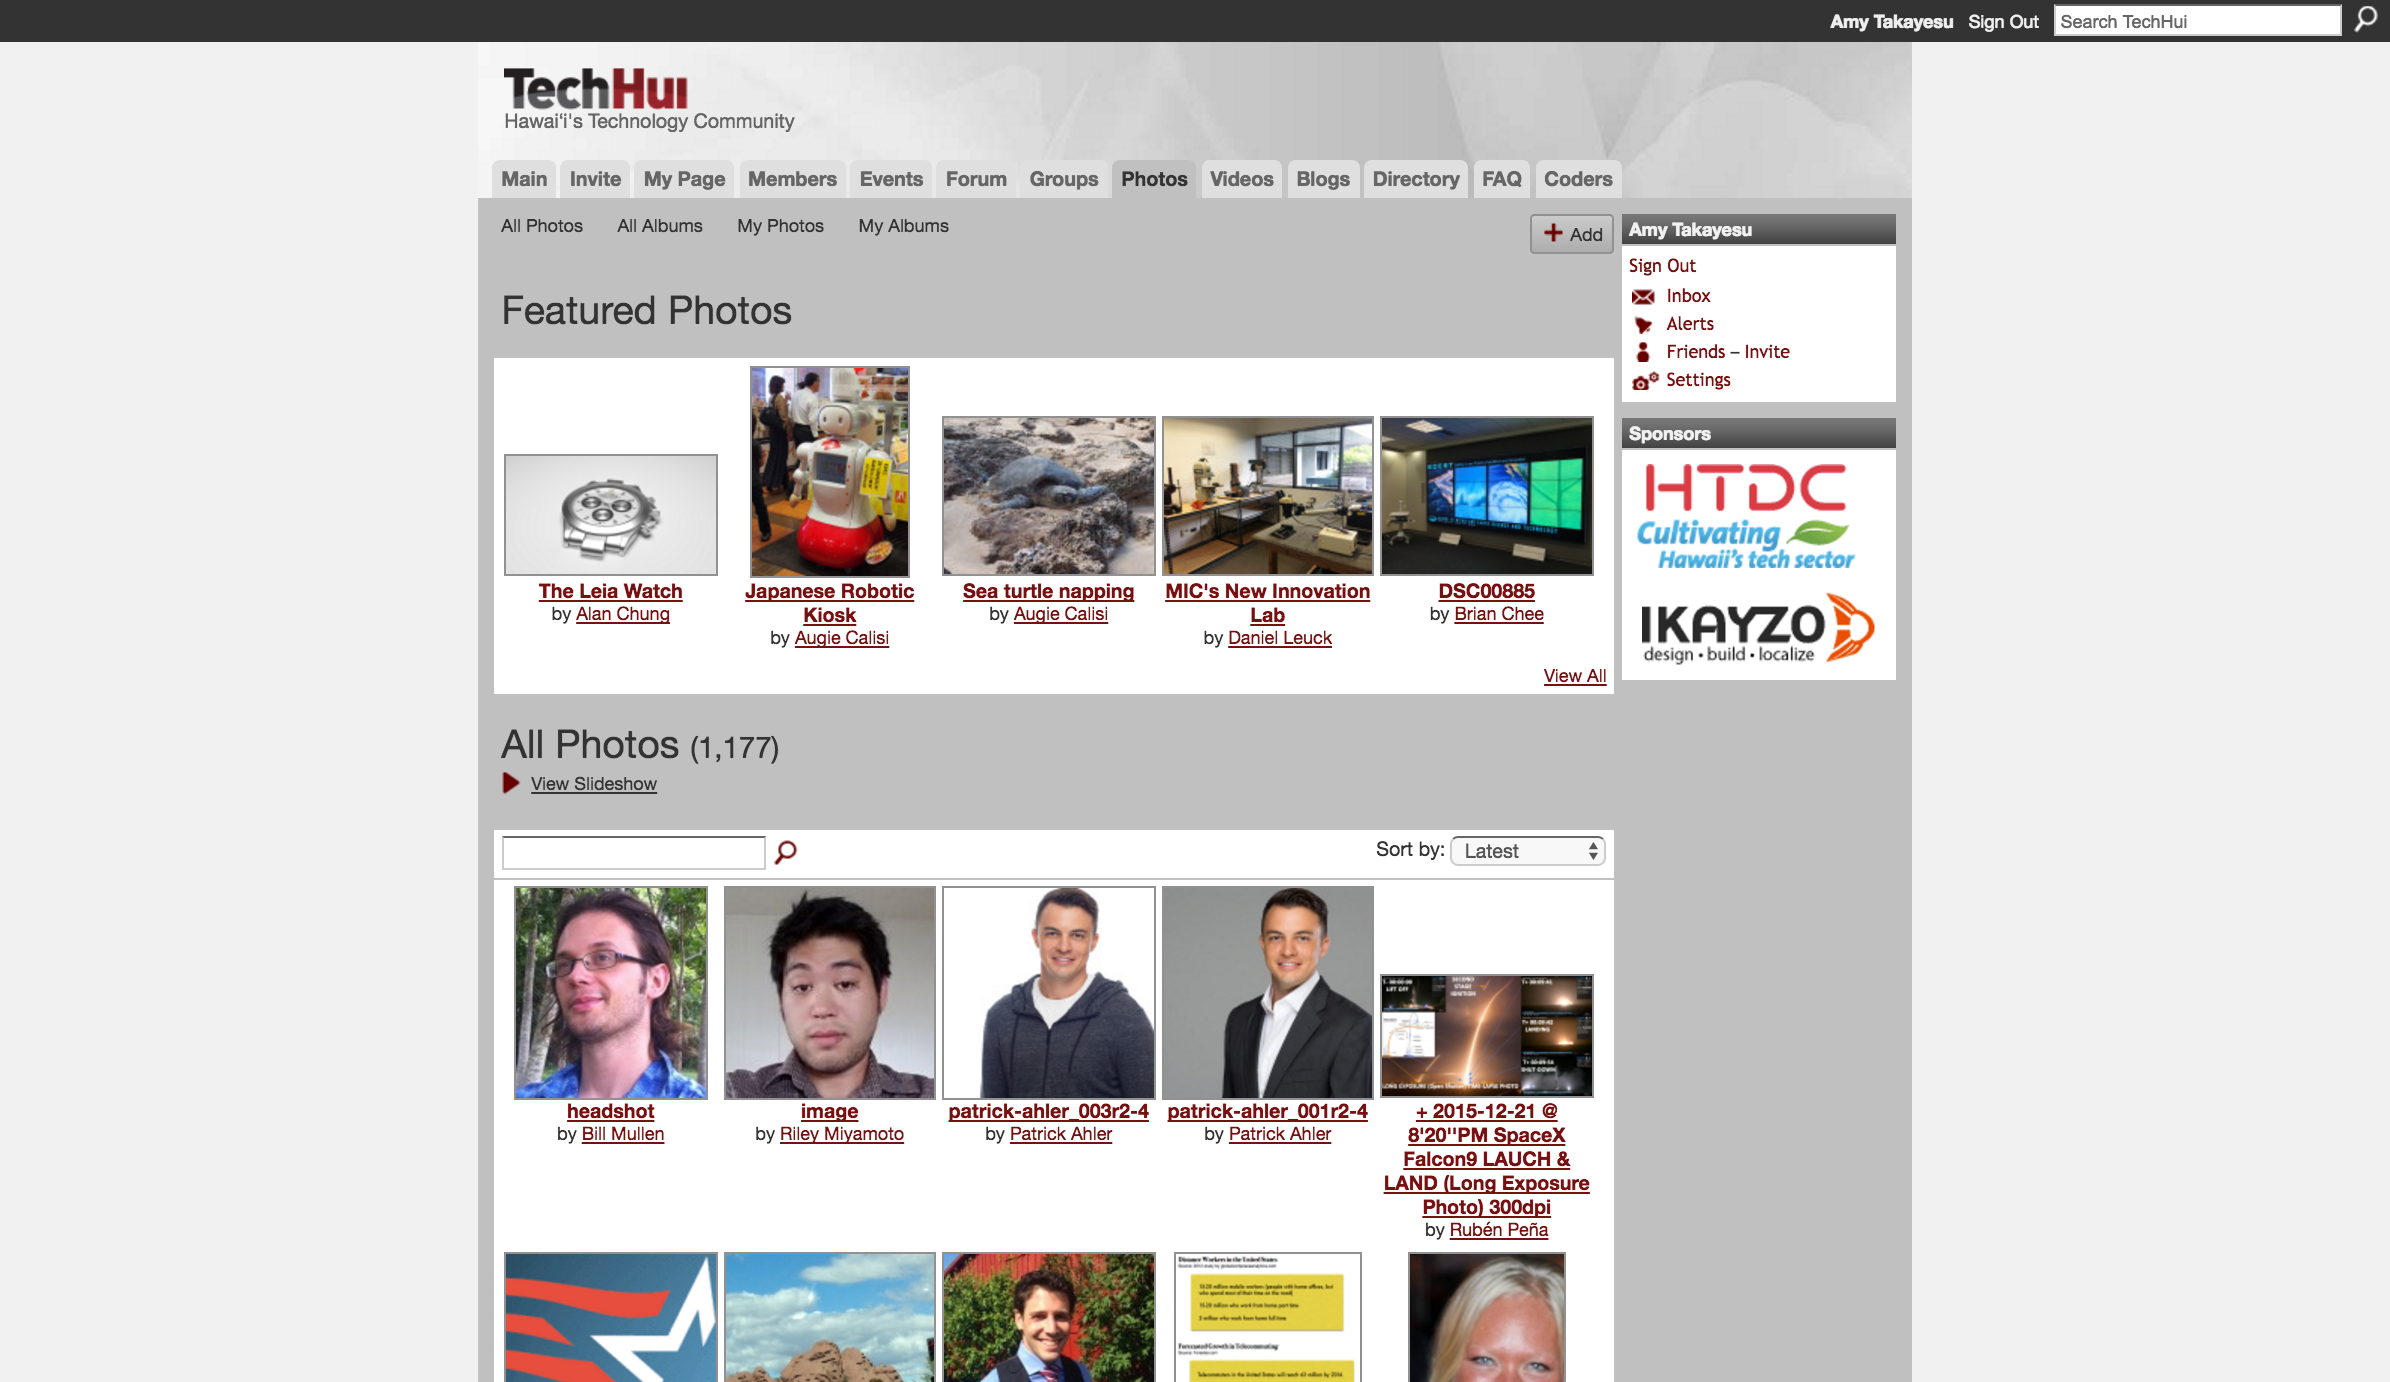
\includegraphics[width=1.0\textwidth]{techhui_photos}
\caption{TechHui photos page. \textit{Source: http://www.techhui.com}}
\end{figure}
\subsubsection{Photos}
On the Photos page, users can easily view all public photos uploaded by users (including profile pictures). Featured photos are included as well. Users can view these photos and comment on them as well. 

\begin{figure}[h]
\centering
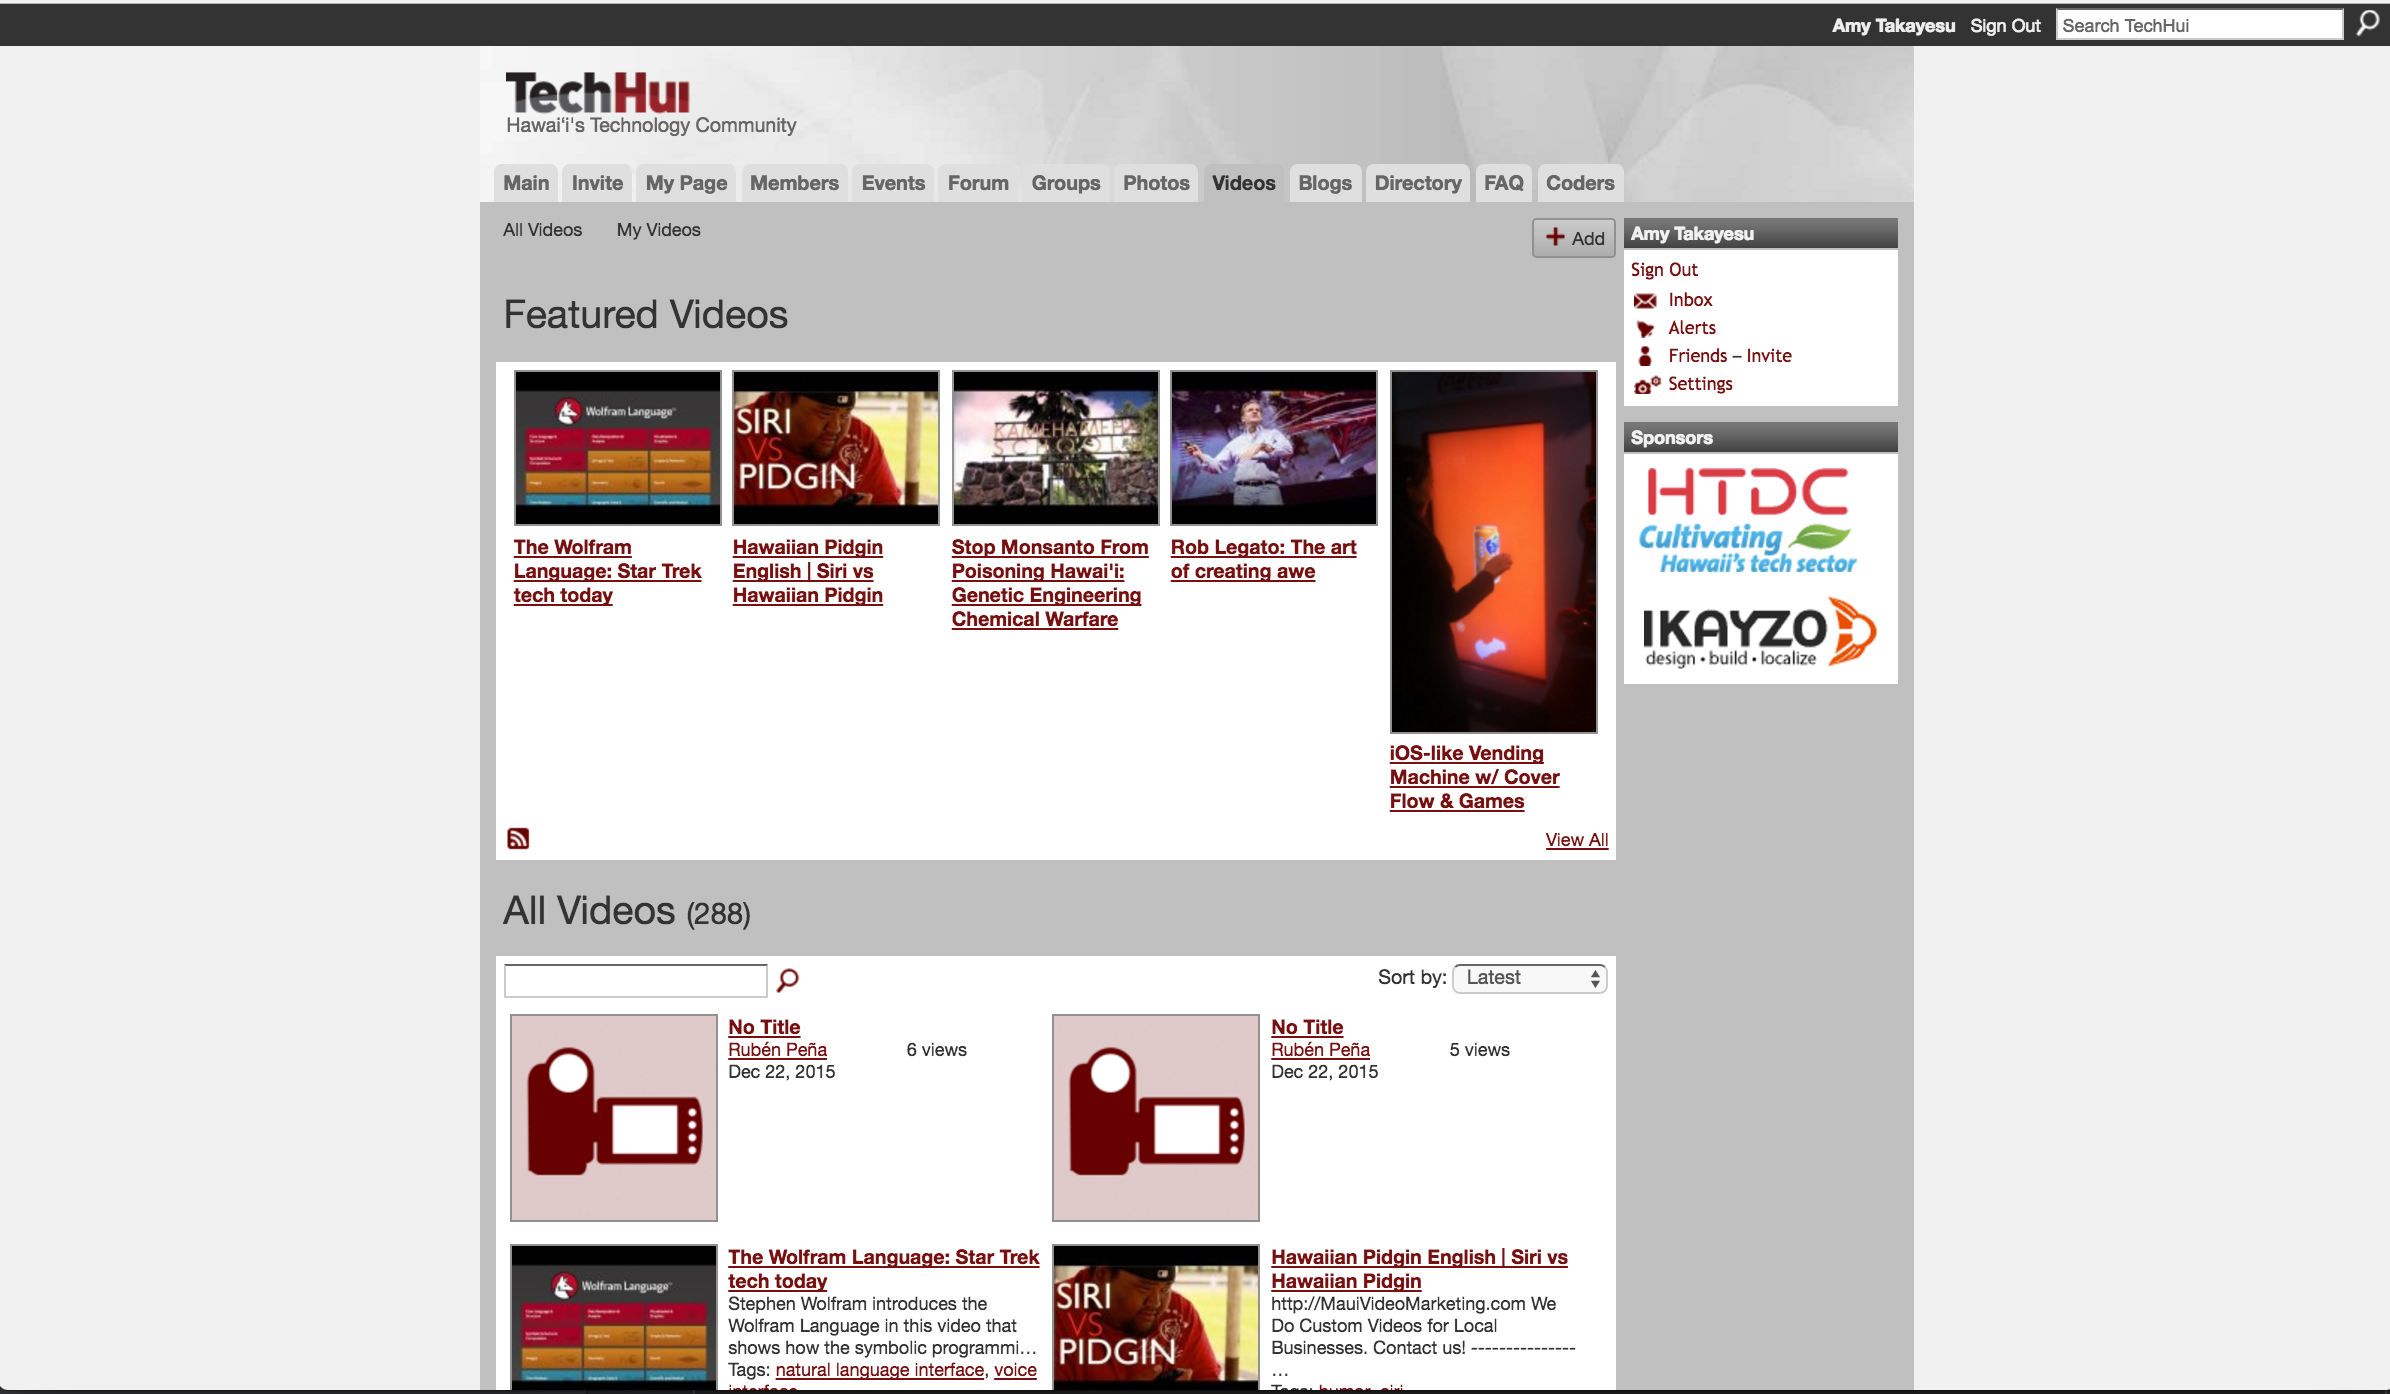
\includegraphics[width=1.0\textwidth]{techhui_videos}
\caption{TechHui videos page. \textit{Source: http://www.techhui.com}}
\end{figure}
\subsubsection{Videos}
On the Videos page, users can easily view all public videos uploaded by users. Featured videos are included as well. Users can view these videos and comment on them as well. 

\begin{figure}[h]
\centering

\includegraphics[width=1.0\textwidth]{techhui_blogs}
\caption{TechHui blogs page. \textit{Source: http://www.techhui.com}}
\end{figure}
\subsubsection{Blogs}
This page displays a feed of all users' blog posts. Posts are also organized by featured posts, latest posts, most popular posts, and monthly archives. Users can click on these blog posts to read them in their entirety and can comment on them as well. 

\begin{figure}[h]
\centering
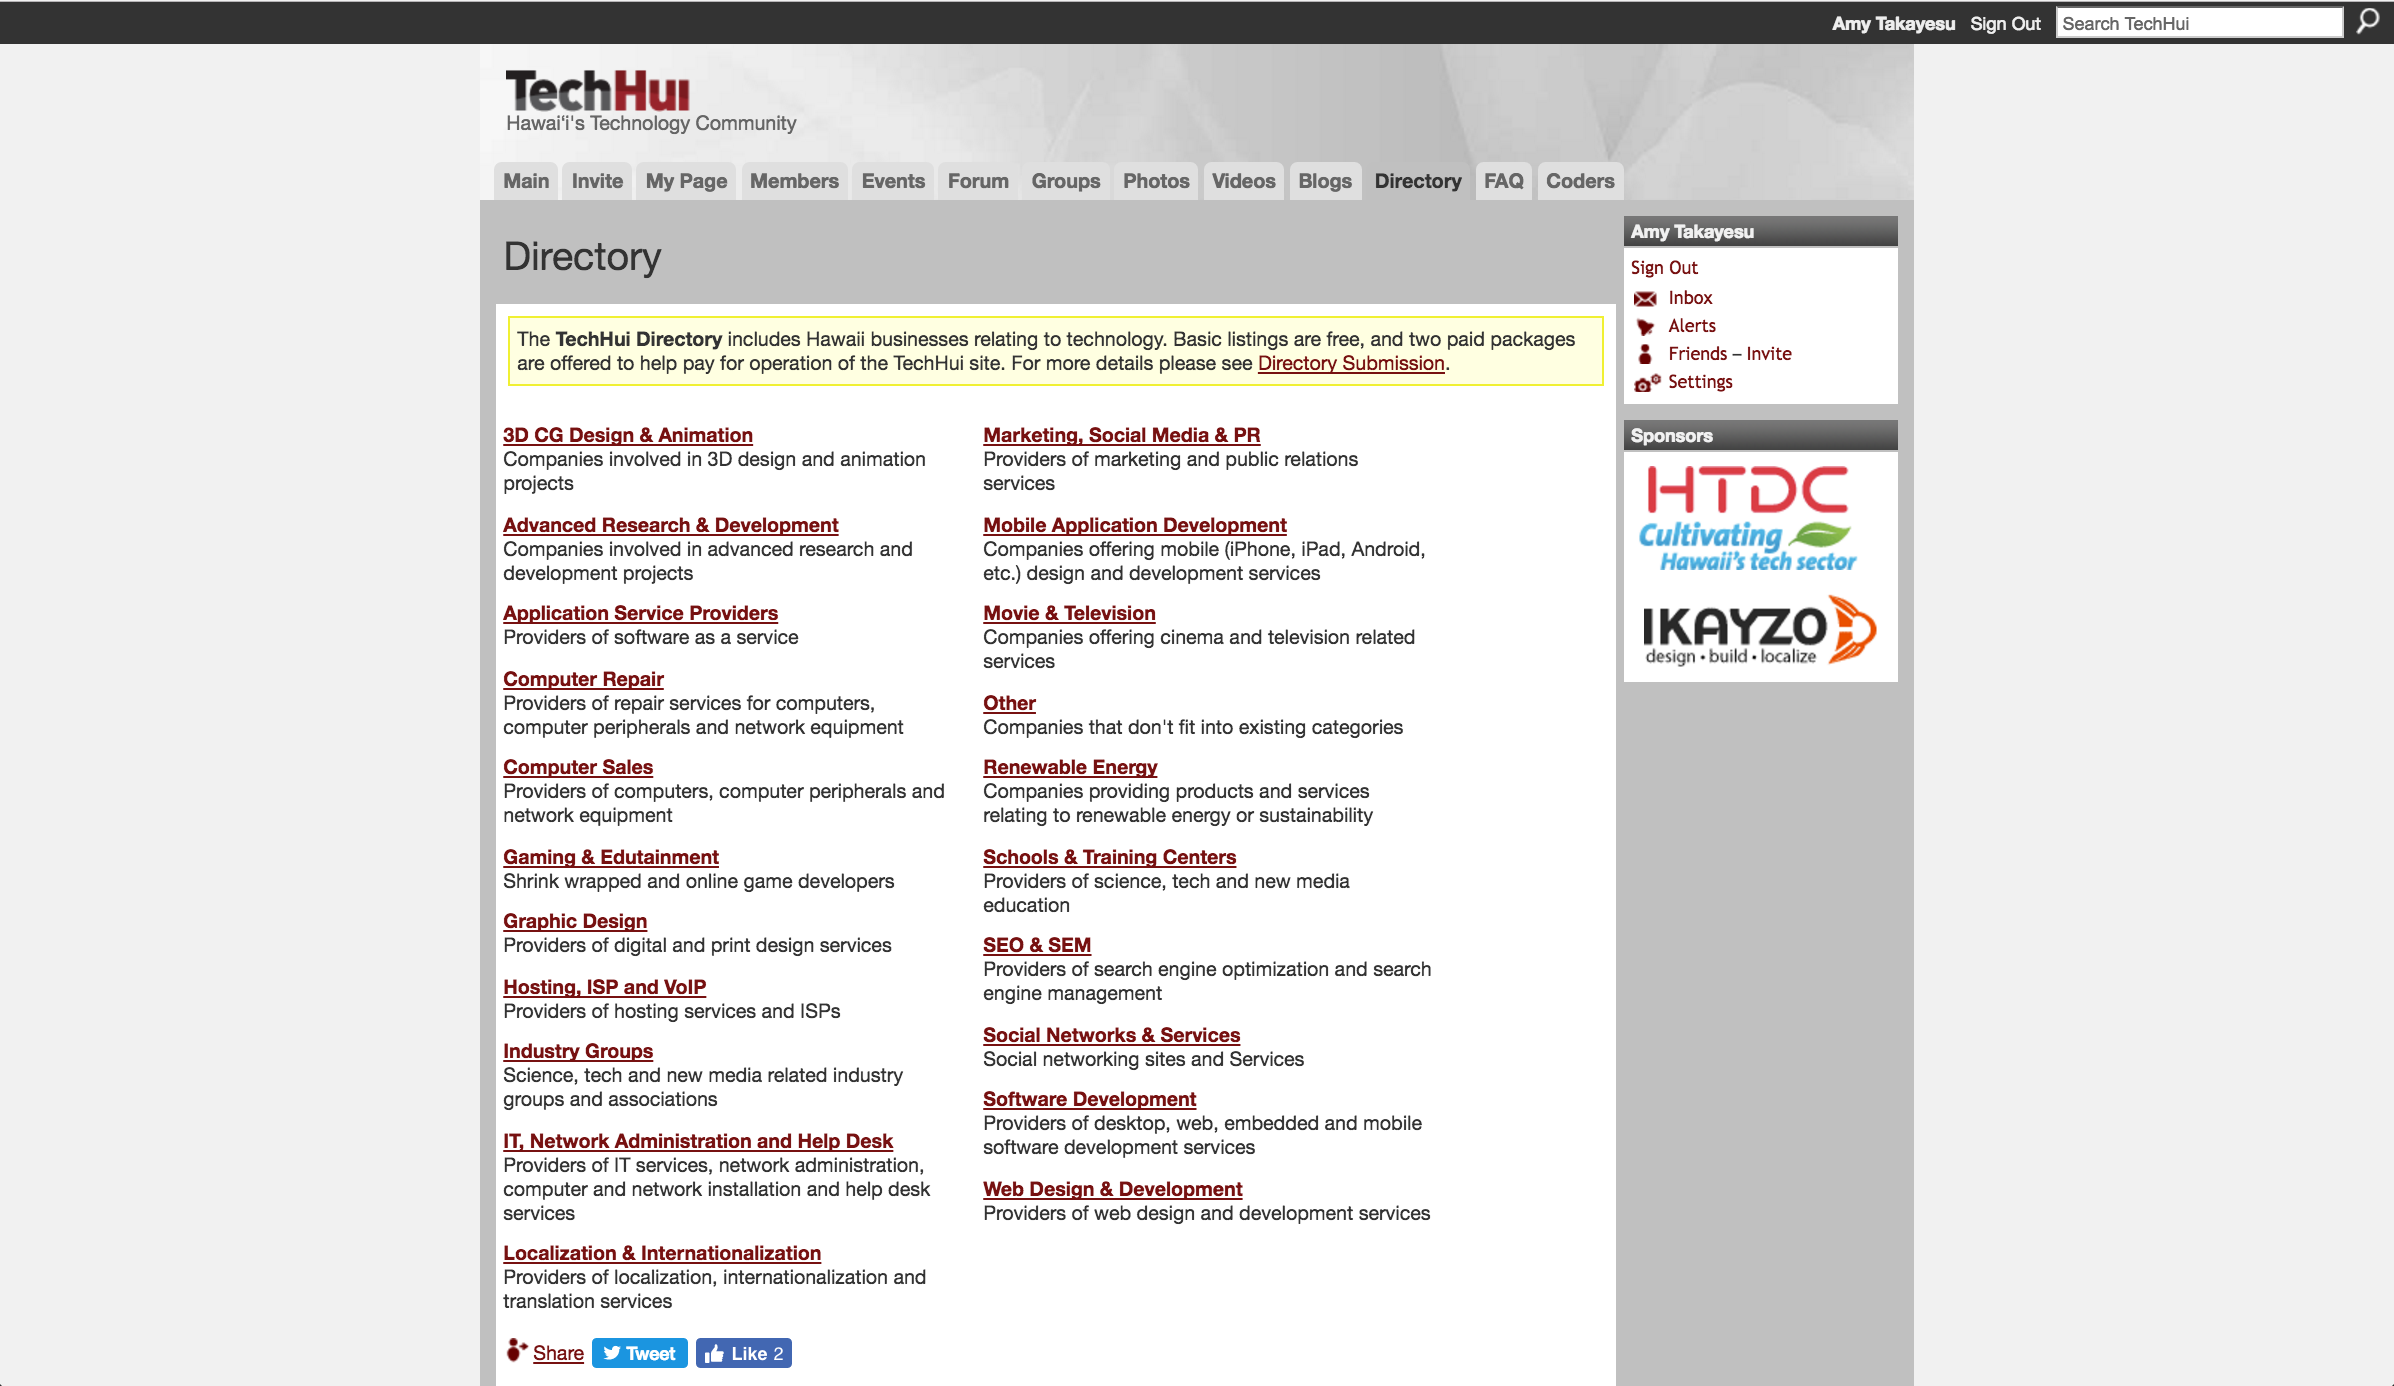
\includegraphics[width=1.0\textwidth]{techhui_directory}
\caption{TechHui directory page. \textit{Source: http://www.techhui.com}}
\end{figure}
\subsubsection{Directory}
This page includes a listing of technology related jobs in Hawaii, organized into 21 subcategories. Users can click on these listings to view more details about the jobs, and also to access external websites.

\begin{figure}[h]
\centering
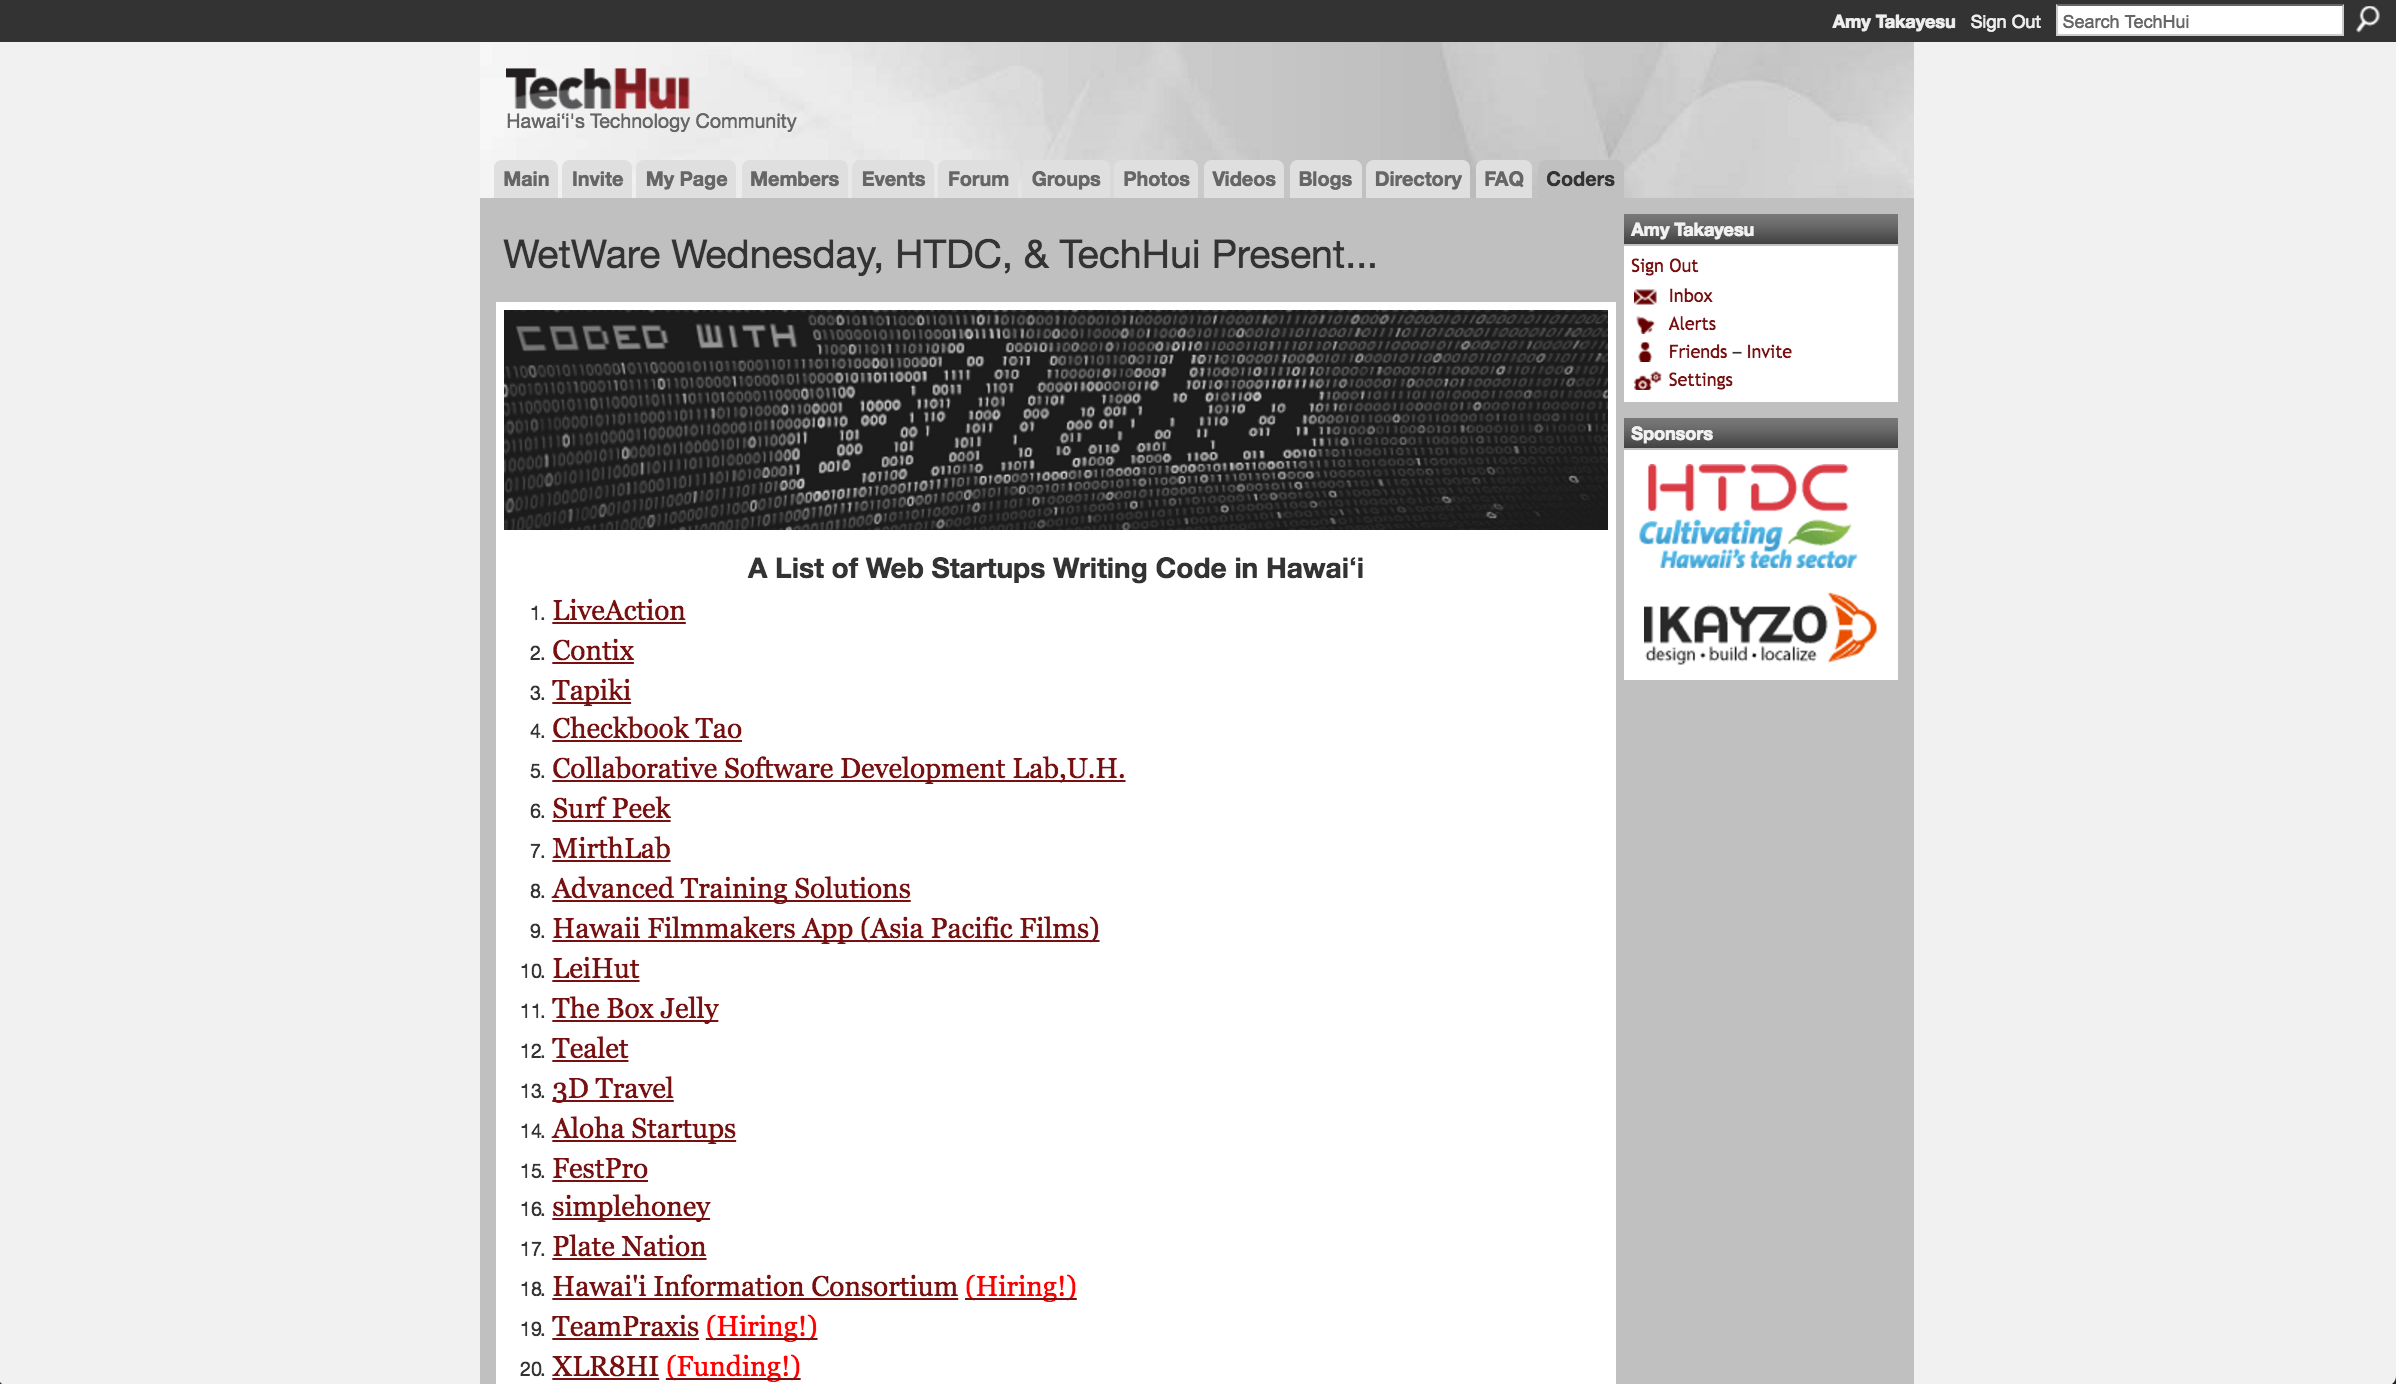
\includegraphics[width=1.0\textwidth]{techhui_coders}
\caption{TechHui coders page. \textit{Source: http://www.techhui.com}}
\end{figure}
\subsubsection{Coders}
This page lists web startups that are writing code in Hawaii. The list contains just the names of the startups, which can be clicked on to learn more at the startup website.

\subsubsection{TechHui and Academic/Professional/Social Engagement}
TechHui caters to a community much smaller than LinkedIn. However, it remains too broad to cater to the specific needs of undergraduate students. TechHui aims to satisfy the needs of a variety of people, with only a small portion of them being current undergraduate students. It is unreasonable to expect TechHui to add features specifically for one group of members. However, if it were reasonable, TechHui ideally could suggest events and people to students based off their goals and interests. It could find ways to encourage students to engage with these events and people, and cultivate strong and healthy relationships between students and the rest of the community. It could provide ways for members to easily know what projects others are working on, and allow members to join projects that they are interested in. In this way, it would be more than just a discussion site, but a strong social network as well. 

\begin{figure}[h]
\centering
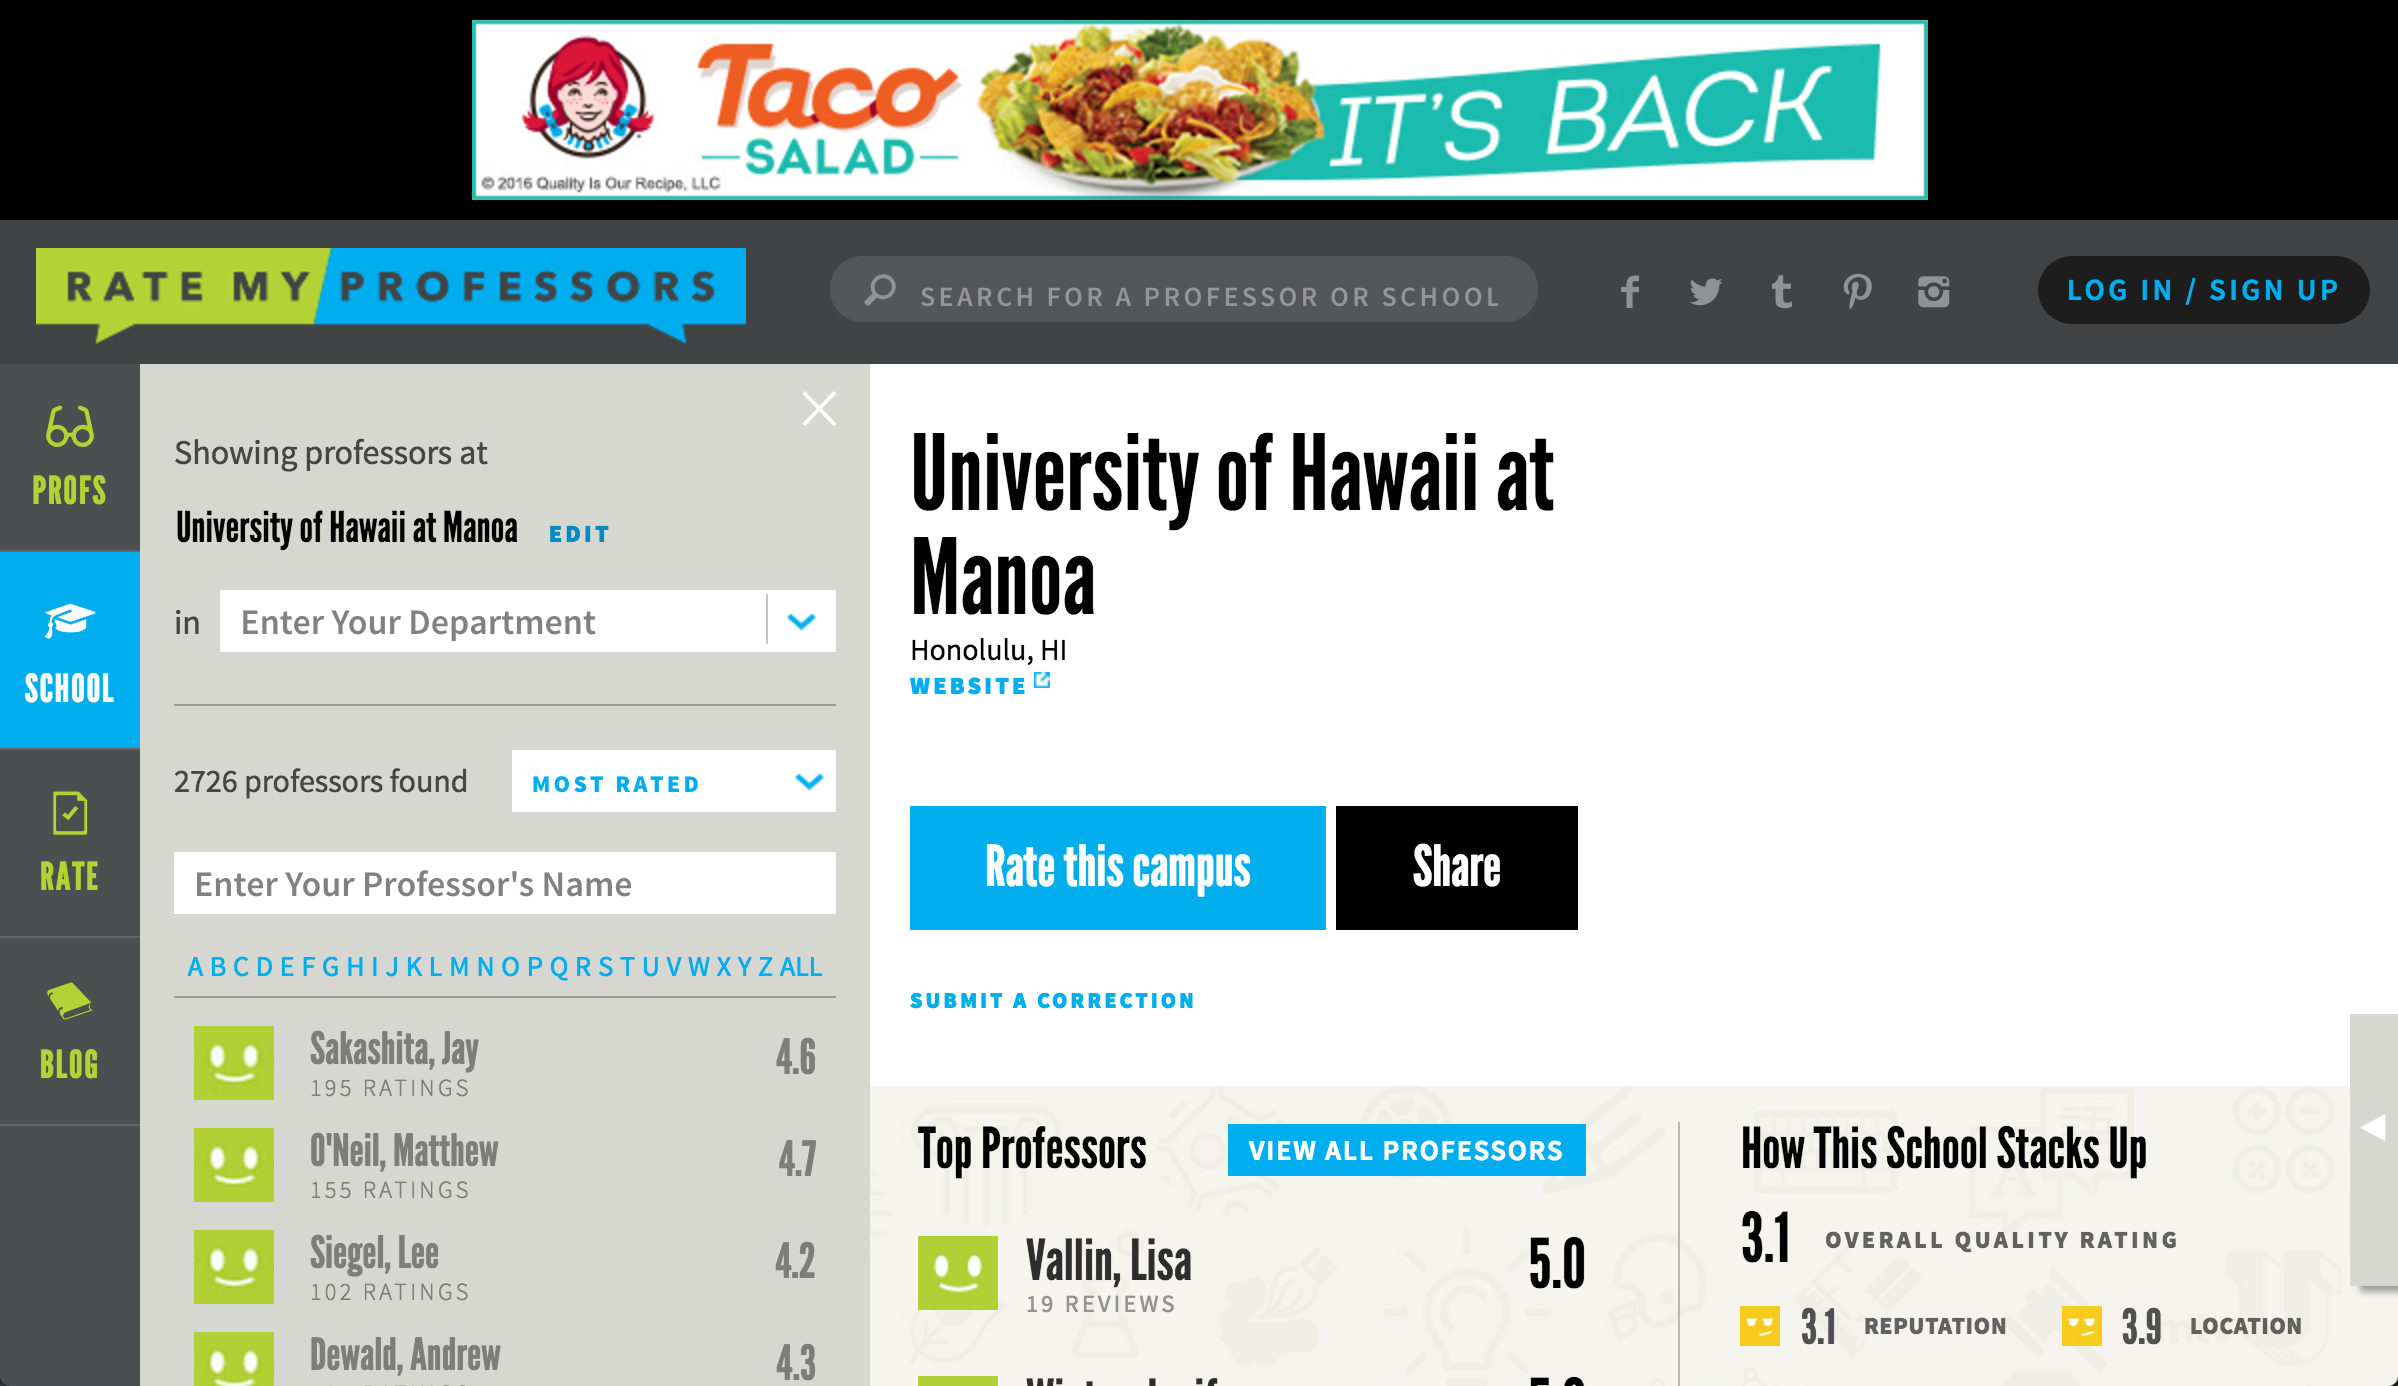
\includegraphics[width=1.0\textwidth]{ratemyprofessor}
\caption{Example Rate My Professor page for UH Manoa. \textit{Source: http://www.ratemyprofessor.com}}
\end{figure}
\subsection{Rate My Professor}
Rate My Professors allows users to communicate and share content with each other by posting reviews of colleges and professors. Although users can create accounts, the reviews are listed as anonymous. Other users can provide feedback on reviews with either a thumbs up (user found this to be useful) or thumbs down (user did not find this to be useful). The site also contains site-generated blog posts and videos, but users cannot directly interact with these.

\subsubsection{Rate My Professor and Academic/Professional/Social Engagement}
Rate My Professor aims to be very disconnected from universities by allowing users to be anonymous and share openly without any direct association to the institution. While this allows users to post without fear of repercussions, it may encourage negative relationships between students and professors. It distances the two groups of people, and instead of providing constructive criticism to the professor, it simply encourages the perpetuation of the opinions of past students. In this way, it does not encourage forward movement. Rate My Professor could improve by becoming integrated with the university so that reviews are no longer anonymous, and students can take full responsibility of their opinions. Additionally, professors will be able to view informative data about their teaching effectiveness, which may allow them to improve over time. In this way, the goal will become to improve all members of the community, rather than to create more distance between them.

\subsection{Other Popular Social Networks and Academic/Professional/Social Engagement}
Social networks have become extremely popular and there are too many of them to describe in detail here. The top fifteen most popular social networks as of September 2016 are Facebook, Instagram, YouTube, Twitter, LinkedIn, Pinterest, Google+, Tumblr, Reddit, VK, Flickr, Vine, Meetup, Ask.fm, and ClassMates. While most of these are not academically focused, they could potentially host an academic environment. Additionally, while RadGrad could be integrated directly into one of these existing social networks (i.e. become a Facebook application), creating a standalone application does not exclude members who do not have a Facebook or are not active on Facebook, it does not depend on the continuing popularity of Facebook, and I believe it may develop a stronger sense of brand. 

\section{Gamification}
Since it would be ineffective and senseless to discuss every existing video game, I conducted a brief informal survey of some ICS students (both undergraduate and graduate students) regarding their current favorite video game. I was able to solicit sixteen responses shown in the table below. In the following section I will discuss four different video games, with each one from a different genre: Role Playing Game (RPG), Multiplayer Online Battle Arena (MOBA), collectible card, First Person Shooter (FPS), and augmented reality. One of the games is my current favorite video game and four of them are popular video games according to the surveyed ICS students. 
\\
\begin{tabular}{ |p{2cm}|p{3cm}|p{5cm}|p{5cm}|}
 \hline
 \multicolumn{4}{|c|}{ICS Students' Favorite Games} \\
 \hline
 Gender & Degree & Favorite Game & Game Genre\\
 \hline
 Male   & Undergraduate    & Seven Knights & RPG\\
 Male   & Undergraduate    & Kerbal Space Program & Space Flight Simulation\\
 Male   & Undergraduate    & League of Legends & MOBA\\
 Female   & Undergraduate    & League of Legends & MOBA\\
 Male   & Undergraduate    & Monster Hunter & RPG\\
 Male   & Undergraduate    & NBA2k7 & Sports\\
 Male   & Undergraduate    & Hearthstone & Collectible Card\\
 Male   & Undergraduate    & RimWorld & Construction Management\\
 Male   & Undergraduate    & Geometry Dash & Arcade\\
 Male   & Undergraduate    & Overwatch & FPS\\
 Female   & Undergraduate    & Pokemon Go & Augmented Reality\\
 Female   & Graduate    & Pokemon Go & Augmented Reality\\
 Female   & Undergraduate    & Minecraft Sky Factory 2.5 & Sandbox\\
 Female   & Graduate    & Call of Duty & FPS\\
 Female   & Undergraduate    & Assassin's Creed & Action/Adventure\\
 Female   & Graduate    & Summoner's War & RPG\\
 \hline
\end{tabular}

\begin{figure}[h]
\centering
\includegraphics[width=1.0\textwidth]{sw}
\caption{Summoners War gameplay}
\end{figure}

\subsection{Summoners War}
Summoners War is a mobile fantasy RPG with over 60 million players worldwide. It is based off a freemium model, with many players playing for free, and many other players playing with in-application purchases. Based off the iTunes Summoners War page, the basic premise of Summoners War is as follows: ``Jump into the Sky Arena, a world under battle over the vital resource: Mana Crystals! Summon over 900 different types of monsters to compete for victory in the Sky Arena! Assemble the greatest team of monsters for strategic victories!"
	As with many games, one of the interesting things about it is it's ability to motivate users into completing several, often tedious and unenjoyable actions, in order to achieve a virtual reward. One of the examples of this is the weekly Arena Rank. The Arena is where players can battle against other players, in an attempt to reach as high a rank as possible. There are different ranks based off the amount of victories and defeats the player has had: Beginner, Challenger, Fighter, Conqueror, Guardian, and Legend. The Arena is often very difficult, and in order to achieve a certain standing, the player must constantly battle others, and set up a solid defense that cannot be defeated by other players. In order to improve one's defense and offense team, a player must spend hours doing grueling tasks, such as gathering magical essences, gaining EXP points to level monsters, and collect ``runes" which can be strategically placed on each monster to improve certain stats. Doing these tasks can take up a significant amount of time and energy. Each week, a player is awarded a certain rank based off their performance in the Arena that previous week. This rank is manifested in the form of a small icon next to the player's name. When players see other players' icons, they are immediately informed of that person's standing in the game, and the player him/herself will be rewarded with feelings of pride and satisfaction.
	
Summoners War also allows players to join guilds in order to receive guild points, which can be used to purchase additional helpful items. Guilds are composed of at most 30 players, and they must strategize and work together in order to move up in rank and gain more points. 

\begin{figure}[h]
\centering
\includegraphics[width=1.0\textwidth]{lol}
\caption{League of Legends gameplay.}
\end{figure}

\subsection{League Of Legends}
League of Legends is a multiplayer online battle arena (MOBA) type of video game and also follows a freemium business model. In this game, the player assumes the character of a summoner who controls a champion with unique abilities, and they battle with a team of other champions against another team of champions (either other live players or computer controlled). The main goal of the game is to destroy the opposing team's nexus, which is a structure at the middle of the team's base and is protected by defensive structures. At the start of each match, all champions start off weak, but they can increase in strength throughout the game by accumulating items and experience. Each match typically lasts from 20-60 minutes. There are three different game modes: Summoner's Rift, Twisted Treeline, and Howling Abyss. Each game mode is similar in that a team of players must work together to accomplish a terminal objective and a victory condition. Each mode also includes smaller intermediate objectives that can help teams to get closer to victory. 
	Opposed to Summoner's War, gold gathered during the match and items purchased with that gold only last for that match, and do not carry over to future matches. Each match begins with each player being more or less equal in terms of advantage, regardless of how much time or effort the player has put in beforehand. 
	However, the game does include other incentives to continue to win games and see personal development. Players get player experiences from playing matches on a single account. As their experience increases, they can ascend from level 1 to 30. Higher level players are given access to different maps, game modes, and additional abilities and features which give players a small boost in battle. 
	
\begin{figure}[h]
\centering
\includegraphics[width=1.0\textwidth]{hearthstone}
\caption{Hearthstone gameplay.}
\end{figure}	
\subsection{Hearthstone}
Hearthstone is a free to play online collectible card video game. It is turn based between two opponents, who use constructed decks of thirty cards, and a selected hero with a unique power. Players can attack the opponent using mana points. The main goal is to reduce the opponent's health to zero. If the player wins, they can earn in-game gold, new cards, or other in-game prizes. Players can use the gold or microtransactions to purchase new cards to improve their decks. There are several different game modes: casual and ranked matches, daily quests, and weekly challenges. Unlike many other popular collectible card games, Hearthstone does not allow players to trade cards. Instead, players can disenchant their unwanted cards into arcane dust, which can then be used to craft new cards of the player's choice. 

\begin{figure}[h]
\centering
\includegraphics[width=1.0\textwidth]{overwatch}
\caption{Overwatch gameplay.}
\end{figure}
\subsection{Overwatch}
Overwatch is a team based multiplayer first person shooter (FPS). Each team has six players, and each player may select one predefined hero character. There are four classes of heroes: Offense, Defense, Tank, and Support. Each hero character has unique movements, attributes, and skills. As the team is being set up, the game will provide advice if the team is unbalanced. However, once the game starts, players can still switch characters after a death or after returning to their home base. The team of heroes work together to secure and defend certain control points and/or escort a payload across the map in a certain amount of point. As players continue to play matches, they can gain rewards that do not affect gameplay, such as character skins and poses. At the end of each match, a server-determined Play of the Game (PotG) is replayed for all players. This play is based off certain factors such as a high scoring moves or effective use of a skill. Up to four individual achievements per team are highlighted, and afterwards players can vote for one to promote. The player who wins the most votes get a reward of experience points. 
	As players gain experience points, they can earn a loot box, which provides certain in-game prizes and in-game currency. If players do not have enough experience points for a loot box, they also have the option to obtain one through a microtransaction. 
	The game supports several different gameplays such as tutorial and practice modes, casual matchmaking, weekly brawls, custom games, and competitive play. Casual matchmaking allows players to play alone or with friends, and are randomly matched against others with similar skill levels. The weekly brawl gameplay was inspired by Hearthstone, and features matches with unique rules, which change weekly. Custom games allow users to have private or public games and can edit different options for that specific match. Competitive mode allows players within a certain region and on a certain platform, to become ranked. This mode is run in 2.5 month seasons. Only players at level 25 or above can participate. Participants also much first play ten preliminary matches which will assign the player a skill rating from 1 to 5000, which is used to create ideal matches. Similarly to the arena battles in Summoners War, there are seven skill ranking tiers: Bronze, Silver, Gold, Platinum, Diamond, Master, and Grandmaster. Players can be demoted to a lower tier or promoted to a higher tier based on their performance. Each competitive win awards a player with in-game currency. Players will also get an additional award based on their final ranking at the end of the season. 
	
\begin{figure}[h]
\centering
\includegraphics[width=1.0\textwidth]{pokemon}
\caption{Pokemon Go gameplay.}
\end{figure}	
\subsection{Pokemon Go}
Pokemon Go is a free-to-play, location-based augmented reality game for mobile devices. Players use their device's GPS to locate, capture, battle, and train virtual monsters known as Pokemon. The Pokemon appear through the device's camera as though they were in the same real-world location as the player. 

Players can customize an avatar, which is displayed throughout the game on a map using the player's current geographical position. The map will show game related locations such as PokeStops and Pokemon gyms. Players can get items from PokeStops such as eggs, Poke Balls, berries, and potions. Users can also equip PokeStops with lures, which can attract wild Pokemon. Pokemon gyms are where players can battle and take over the gym in a ``king of the hill" style. These PokeStops and Pokemon gyms are usually located at real-world places of interest. 

Different types of Pokemon are located in different areas of the world. For example, water-type Pokemon are typically found near bodies of water. Players can capture wild Pokemon by ``throwing a Poke Ball" (making a swiping motion on the device) at the Pokemon. When the Pokemon is caught, the player additionally receives stardust and/or candies, depending on the type of Pokemon. These items can be used to raise the Pokemon's combat power (CP). 

The ultimate goal of the game is to capture and evolve all 151 Pokemon. However, throughout the game, there are also many other ways for players to gain experience points. Players can increase in level, and at level 5, they can join one of three teams: Team Valor, Team Mystic, or Team Instinct. These teams play a role when battling at the Pokemon gyms. 

\subsection{Gamification and Academic/Professional/Social}
Clearly there are certain aspects about popular video games that make them so enjoyable, addictive, and satisfying to so many people. Even the two students who initially declared that they "don't have time for games" or simply just don't play games eventually admitted that they did play Pokemon Go at one point. All four games discussed above have a few things in common: multiplayer, small and large rewards throughout the game, additional rewards given simply for putting in time, and the persistence of the player. Four of the five games also include a team aspect which encourages players to work together to advance individually. 

The multiplayer aspect of the games allows players to interact with and become competitive with other players. Rather than beating one's own score, these games allow players to compare themselves with others and advance relative to other players, rather than simply advancing relative to their past selves. Multiplayer games encourage healthy competition, which can cause players to become more motivated.   

The format of the rewards in these games suggest that small rewards as well as large rewards throughout the game, given for a diverse amount of tasks, continues to motivate players and make sure that they do not get discouraged. These awards are often just ranks or an in-game item that can help the player to improve. 

Another similarity in the four games discussed above is the rewards given to players simply for putting in time to play (i.e. EXP points). While players who constantly lose may feel unmotivated and lose interest, if they are given some kind of point just for trying, it makes their attempts seem less fruitless. Players should be encouraged to play, and even more so if they encounter problems. 

The persistence of the player in these video games allows players to continuously improve over time, rather than starting anew with each game. When players can see their improvements, they can be reminded of their past progress, and be encouraged to continue the progress, regardless of how grueling it may be. Once users see that they have done it before, they will know that they can do it again. 

Finally, the team aspect of many of these games suggest that many players enjoy working together with other players to achieve both team and individual goals. This shows that when people work together, they can become stronger both as a team and individually.